\chapter{Convección Mixta en Flujos Completamente Desarrollado}


El propósito de este capítulo es mostrar, vía simulaciones numéricas, cómo la flotabilidad o boyancia modifica un flujo turbulento plenamente desarrollado en un canal de placas paralelas. Se utiliza para esto simulaciones DNS que cubren un extenso espectro de números de Reynolds, Richardson y Prandtl, lo que permite examinar la evolución desde convección forzada hasta convección natural. Tras describir los casos y las variables adimensionales de referencia, se presentan (i) magnitudes estadísticas de primer y segundo orden, (ii) la influencia del número de Prandtl sobre las subcapas viscosa y térmica, (iii) el número de Nusselt y (iv) el factor de fricción de Darcy.

\textcolor{red}{Falta agregar las principales conclusiones}

\newpage

\section{Casos simulados} 

Los resultados de las simulaciones realizadas en este capítulo corresponden a un flujo completamente desarrollado tanto térmica como hidrodinámicamente. Se emplearon Re$_o$=2100, 3150, 4278, 5000, Pr=0.071, 0.71 y valores de Richardon en el rango 0.04 $\lesssim$ Ri$_b$ $\lesssim$ 106. Desde una perspectiva física, la interpretación de estos números adimensionales puede resumirse así: un aumento del número de Reynolds implica una menor viscosidad cinemática y, por tanto, una difusión más rápida del momento dentro del fluido; un incremento del número de Prandtl señala una reducción de la conductividad térmica; mientras que un mayor número de Richardson denota un crecimiento en el flujo de calor.

En la Figura \ref{fig:map_flow_regime} se expone un ``mapa'' del régimen de flujo donde se gráfica el número de Reynolds \textit{bulk}\footnote{Número de Reynolds basado en la velocidad \textit{bulk} y el diámetro hidráulico: $Re^D_b = 8/3 \hspace*{1mm} Re_o$} versus el número de Richardson \textit{bulk} y se muestran las simulaciones realizadas en este trabajo. Es oportuno precisar que, como hipótesis inicial, se supone que ambos fenómenos actúan de forma independiente; no obstante, tal independencia no está necesariamente garantizada. Cabe destacar, además, que en este trabajo se analiza la transición de un régimen a otro, en el cual el flujo se vuelve inestable y puede manifestar intermitencia y/o turbulencia \cite{chen2003direct}. Aceptando provisionalmente que la interacción entre los fenómenos es despreciable y tomando como referencia el diagrama de Moody \cite{white}, se presenta lo siguiente:

\begin{itemize}
	\item para valores de Re$^D_b$ $<$ 2000 el régimen es laminar,
	\item si 2000 $\lesssim$ Re$^D_b$ $\lesssim$ 4000 el régimen es de transición,
	\item y si Re$^D_b>$ 4000 el régimen es turbulento.
\end{itemize}
Por otra parte, el fenómeno de convección es \cite{incropera,cengelheat}:

\begin{itemize}
	\item forzado si Ri$_b<$ 0.1,
	\item mixto si 0.1 $<$ Ri$_b$ $<$10,
	\item y natural si Ri$_b$ $>$10.
\end{itemize}

\begin{figure}[H]
  \centering
    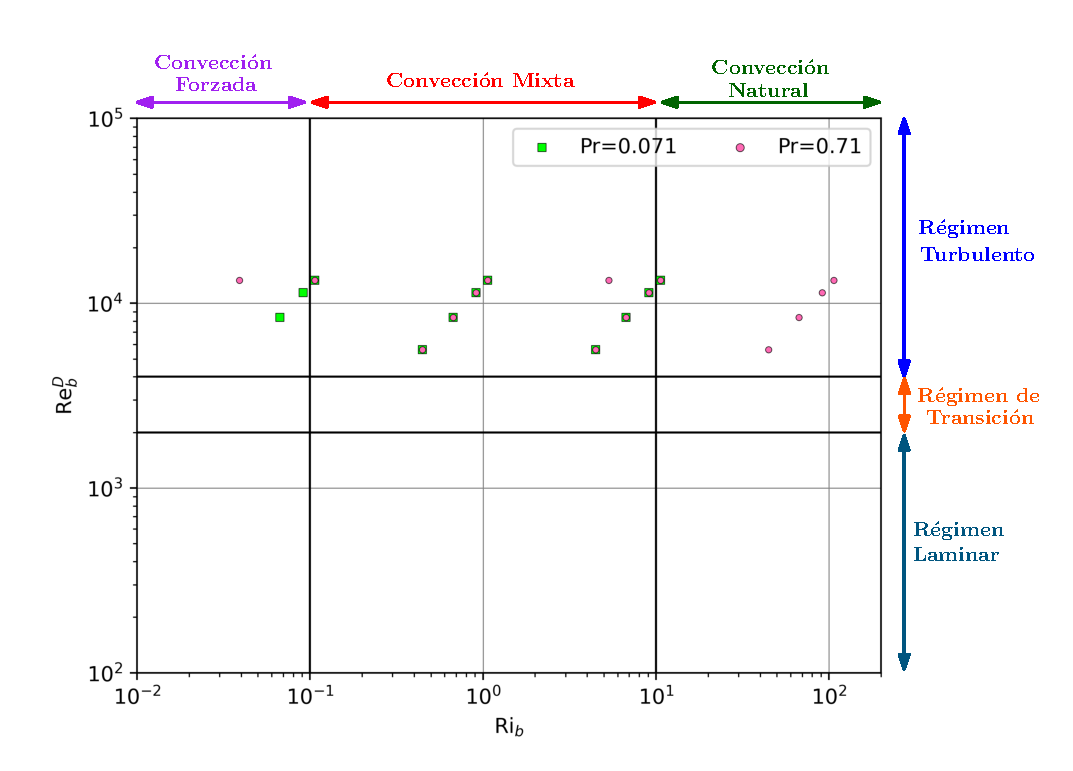
\includegraphics[width=0.8\textwidth]{figures/cap5/map.eps}
  \caption{Mapa de regímenes en el plano $Re^D_b$–$Ri_b$. Se señalan las zonas laminar, de transición y turbulenta, así como los dominios de convección forzada, mixta y natural.}
  \label{fig:map_flow_regime}
\end{figure}

De esta manera, basados en el diagrama de Moody, la totalidad de casos se encuentra en un régimen de flujo turbulento. En su mayoría, los casos se encuentran en flujo de convección mixta, sin embargo, se cuenta con casos donde predomina la convección forzada, y otros donde domina la convección natural. Esto brinda un espectro amplio para el análisis del problema.

\section{Magnitudes de Primer y Segundo Orden}

En esta sección se analiza la influencia de la fuerza boyante en las magnitudes estadísticas de primer y segundo orden. Para tal fin, se consideran, únicamente, los casos Re$_o$=5000 y Pr=0.71. El aumento de la fuerza boyante, o el número de Ri$_b$, equivale a aumentar el flujo de calor. En otras palabras, el aumento de la boyancia en el sistema físico puede interpretarse como aumentar la energía térmica que se le entrega a través de las paredes cuando el fluido es ascendente\footnote{También es equivalente a quitarle energía térmica (enfriar las paredes) cuando la dirección del flujo es descendente.}.


\subsection{Perfiles de velocidad y de temperatura} \label{sec:velo_temp}

En la Figura \ref{fig:ux-Re5000-Pr071} se presentan los perfiles medios de velocidad  \textit{streamwise}\footnote{Es decir, en la dirección de la corriente.} para distintos números de Richardson. En dichos perfiles pueden distinguirse con claridad los tres regímenes de convección. Conforme se intensifica la fuerza boyante, las curvas adoptan una configuración en ``M'', en concordancia con lo reportado por otros autores \cite{you2003direct, zhou2024direct}. A diferencia del caso de convección exclusivamente forzada, el máximo de velocidad deja de situarse en la línea central del canal y se desplaza progresivamente hacia la pared a medida que aumenta Ri$_b$,\cite{carr1973velocity, steiner1971reverse, zhou2024direct}, originando dos máximos locales en lugar del único pico característico del flujo puramente forzado. Este comportamiento puede interpretarse cualitativamente del siguiente modo: en las proximidades de la pared el fluido se encuentra a mayor temperatura lo que implica menor densidad; en consecuencia, la fuerza boyante acelera el flujo en esa región y, por conservación de masa, el fluido ubicado en la zona central experimenta una desaceleración.

\begin{figure}[H]
  \centering
  \subfloat[]{
    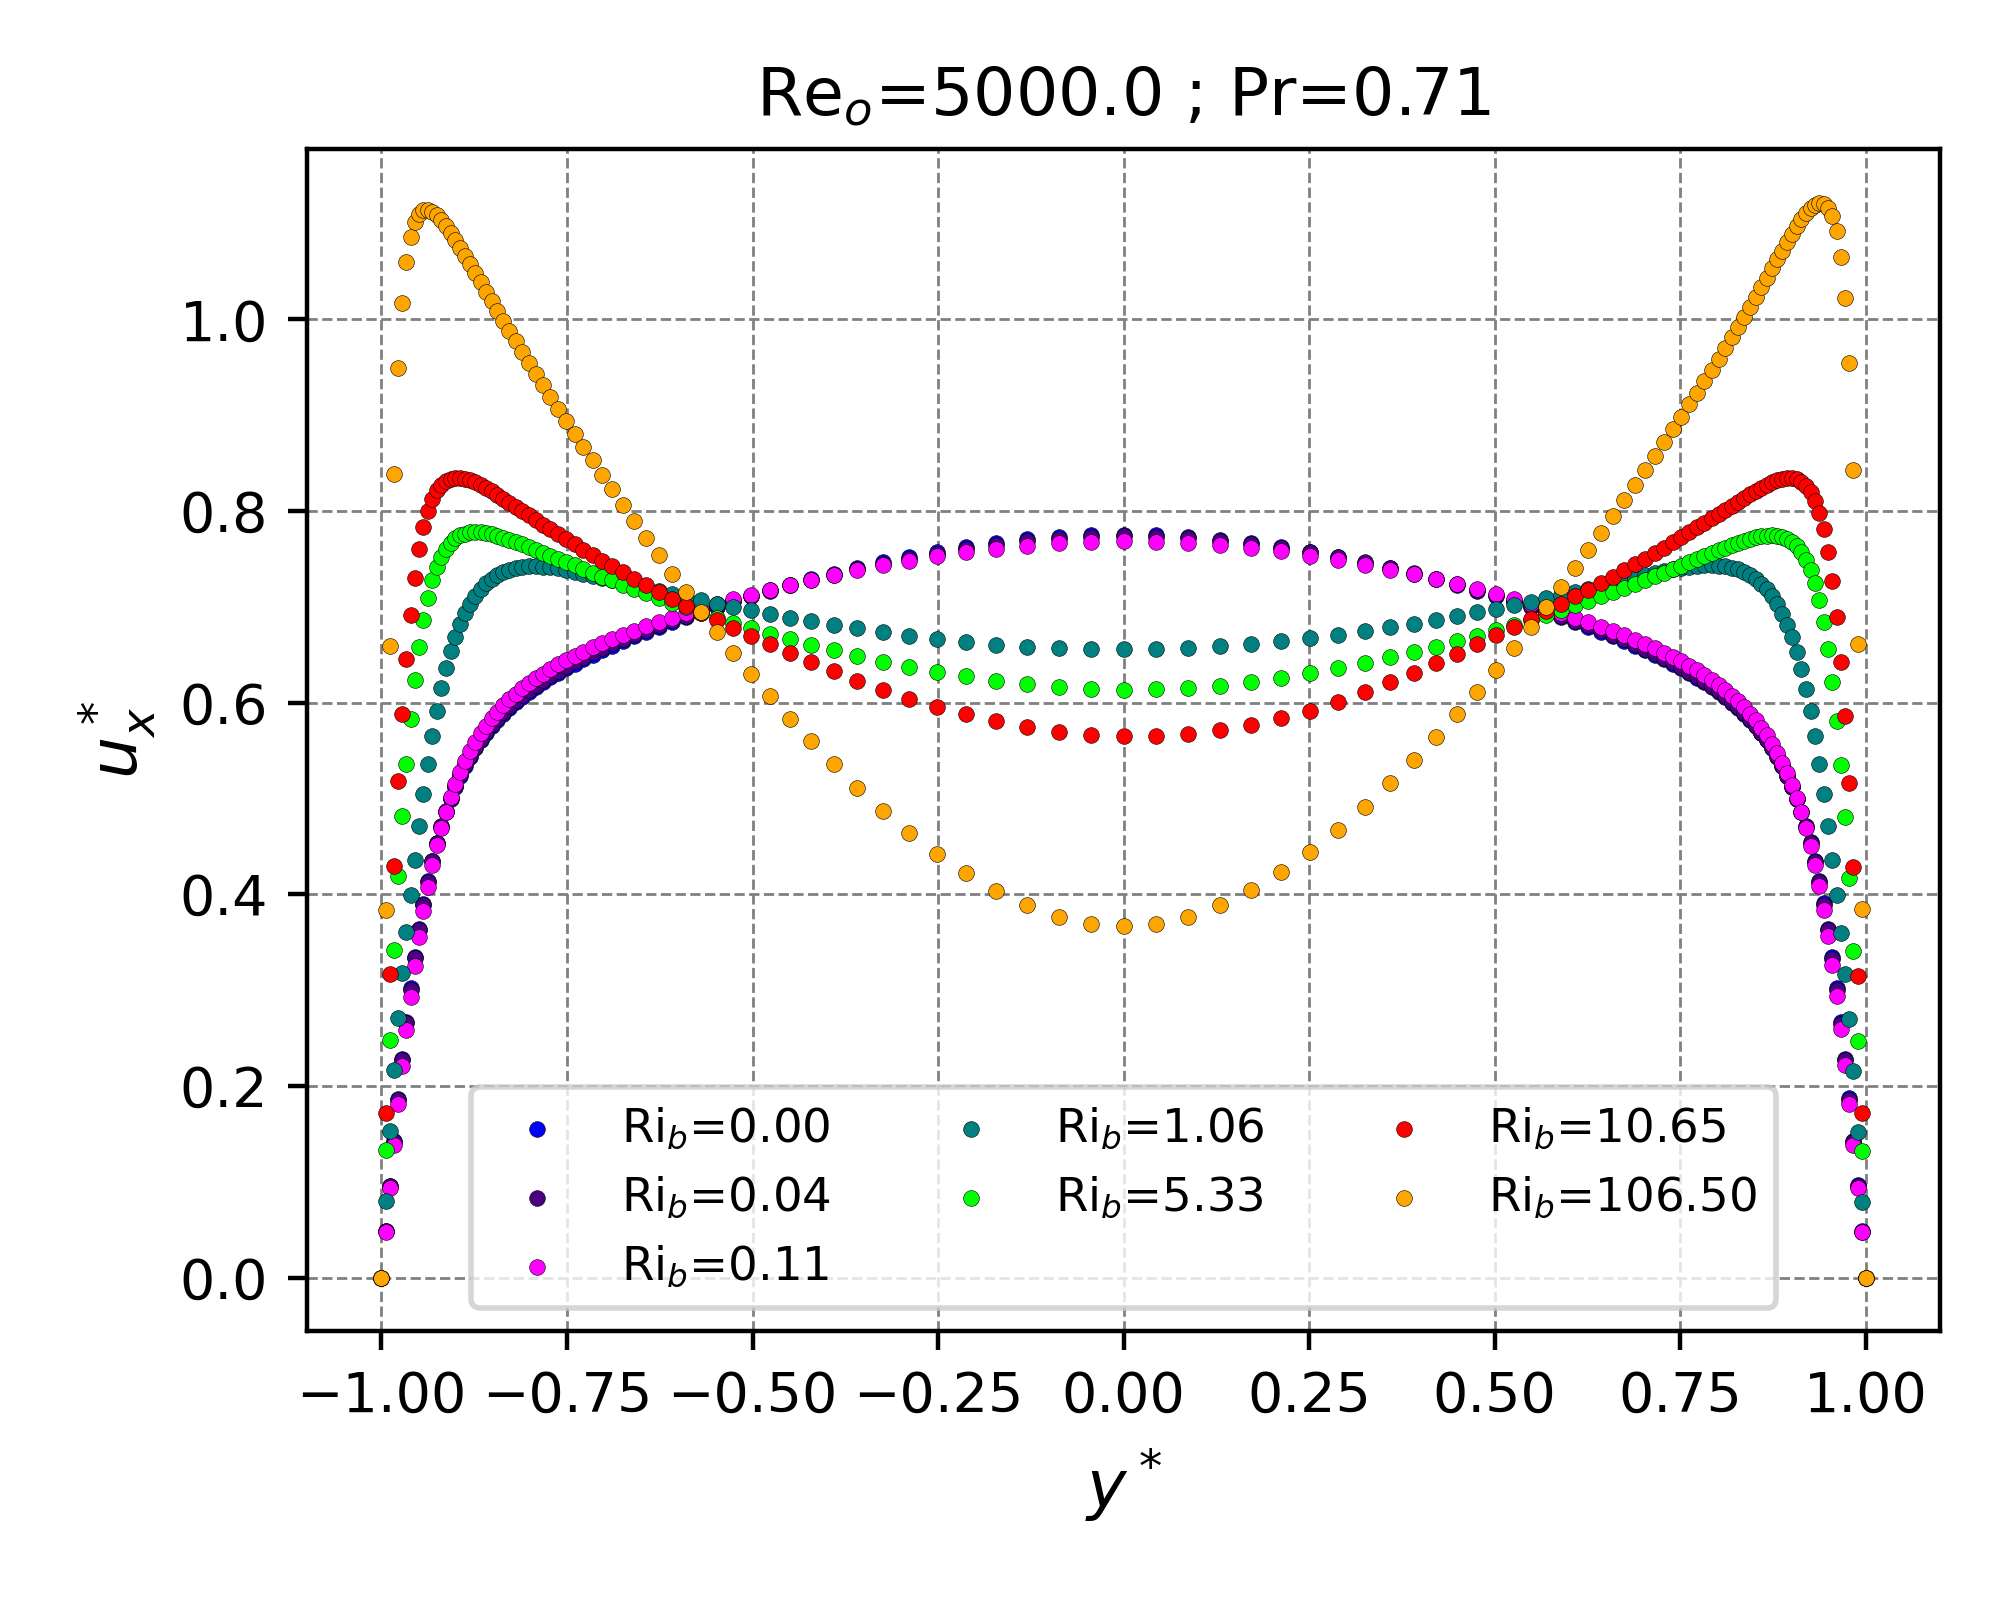
\includegraphics[width=0.49\textwidth]{figures/cap5/Re5000-Pr071/ux_mean_profile.png}
    	\label{fig:ux-Re5000-Pr071}}
  \subfloat[]{
    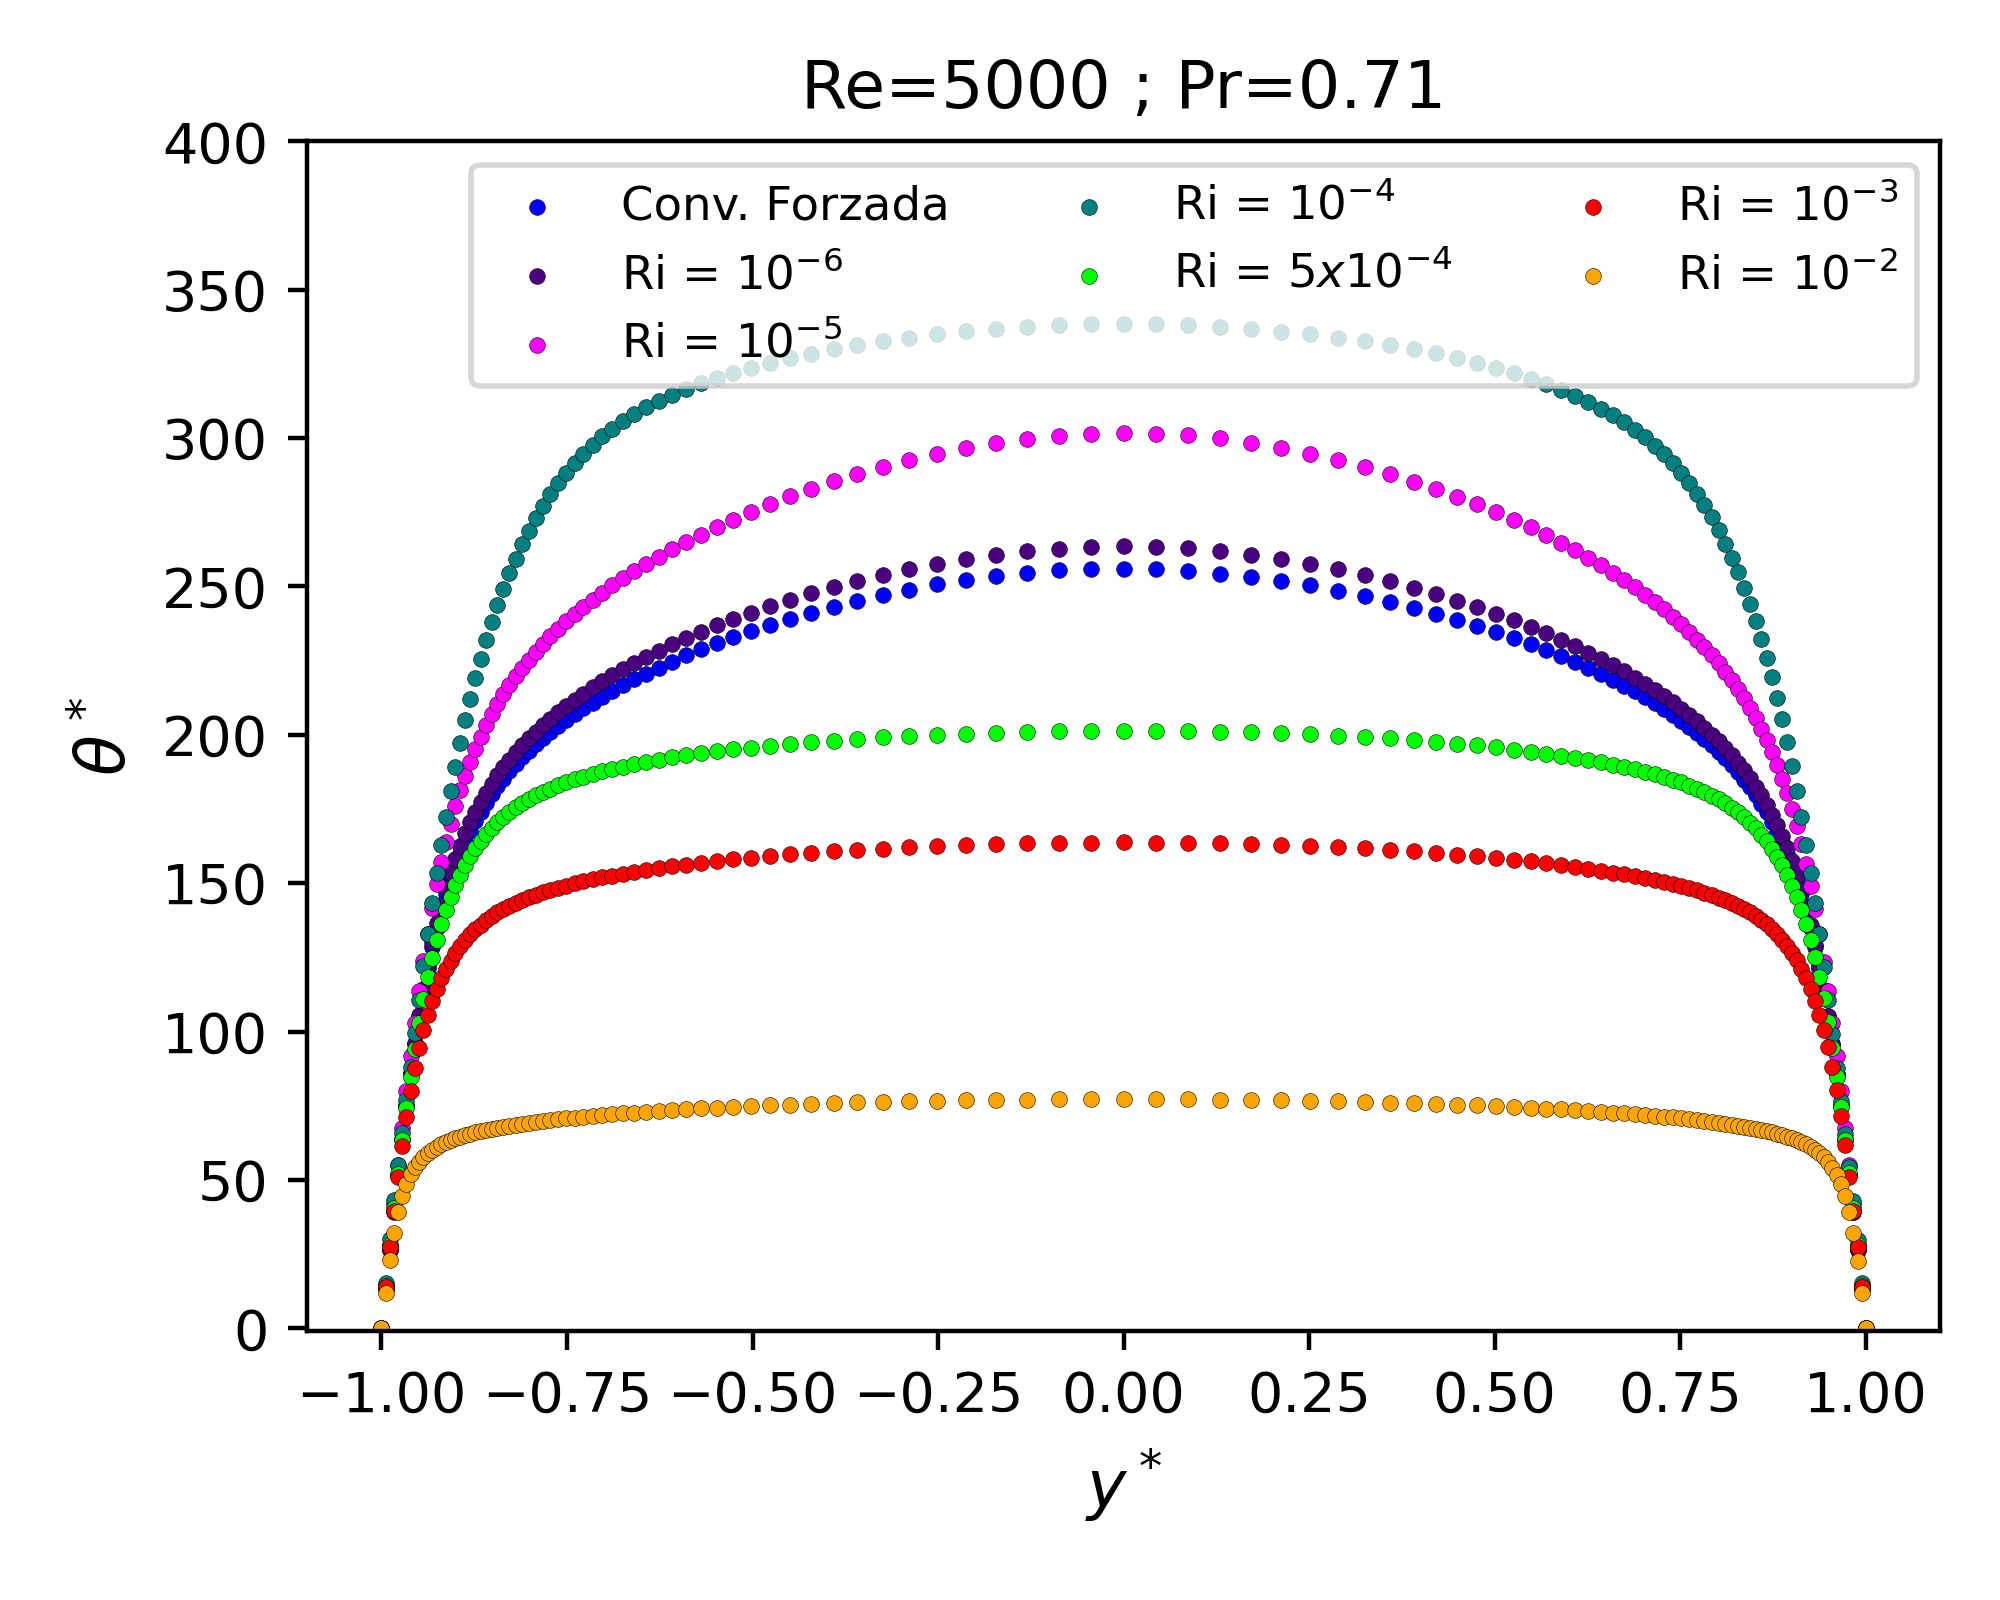
\includegraphics[width=0.49\textwidth]{figures/cap5/Re5000-Pr071/phi_mean_profile.png}
    	\label{fig:phi-Re5000-Pr071}}
  \caption{Perfiles medios adimensionales de \textbf{(a)} velocidad y \textbf{(b)} temperatura, para varios Ri$_b$.}
\end{figure}

Por otra parte, la Figura \ref{fig:phi-Re5000-Pr071} presenta los perfiles medios de temperatura adimensional. A diferencia de los perfiles de velocidad, estos no exhiben la configuración en ``M'' al igual que reportan otros autores \cite{you2003direct, steiner1971reverse}. Los casos pueden clasificarse, en primera instancia, en dos conjuntos:

\begin{itemize}

\item[\textbf{(I)}] valores de Ri$_b$ comprendidos entre 0.04 y 1.06,

\item[\textbf{(II)}] valores de Ri$_b$ entre 5.33 y 106.5.

\end{itemize}
Además, ambos conjuntos exhiben comportamientos físicos claramente diferenciados. Esta distinción se analizará en detalle a lo largo de la presente sección.

En el primer conjunto se aprecia un aumento del perfil adimensional respecto al caso de conveccion forzada, lo que equivale a un descenso de la temperatura dimensional. Cuando la fuerza boyante se intensifica (conjunto \textbf{II}) la temperatura adimensional disminuye, lo que indica un aumento en la temperatura dimensional del fluido. Asimismo, en este segundo conjunto, los perfiles presentan una forma ``achatada'' en el seno del canal que puede interpretarse cualitativamente a partir de sus perfiles de velocidad: la diferencia de velocidades entre la región próxima a la pared y el centro del canal favorece la mezcla del fluido y, por consiguiente, conduce a una distribución térmica más homogénea.




%################################################################################
% MOSAICOS DE TEMPERATURE Y VELOCIDAD UX. 
% Hasta no corregir todo lo demas, esto no se hace 

%\newpage
%
%\begin{figure}[H] % usa [H] solo si necesitas anclarla y tienes \usepackage{float}
%  \centering
%  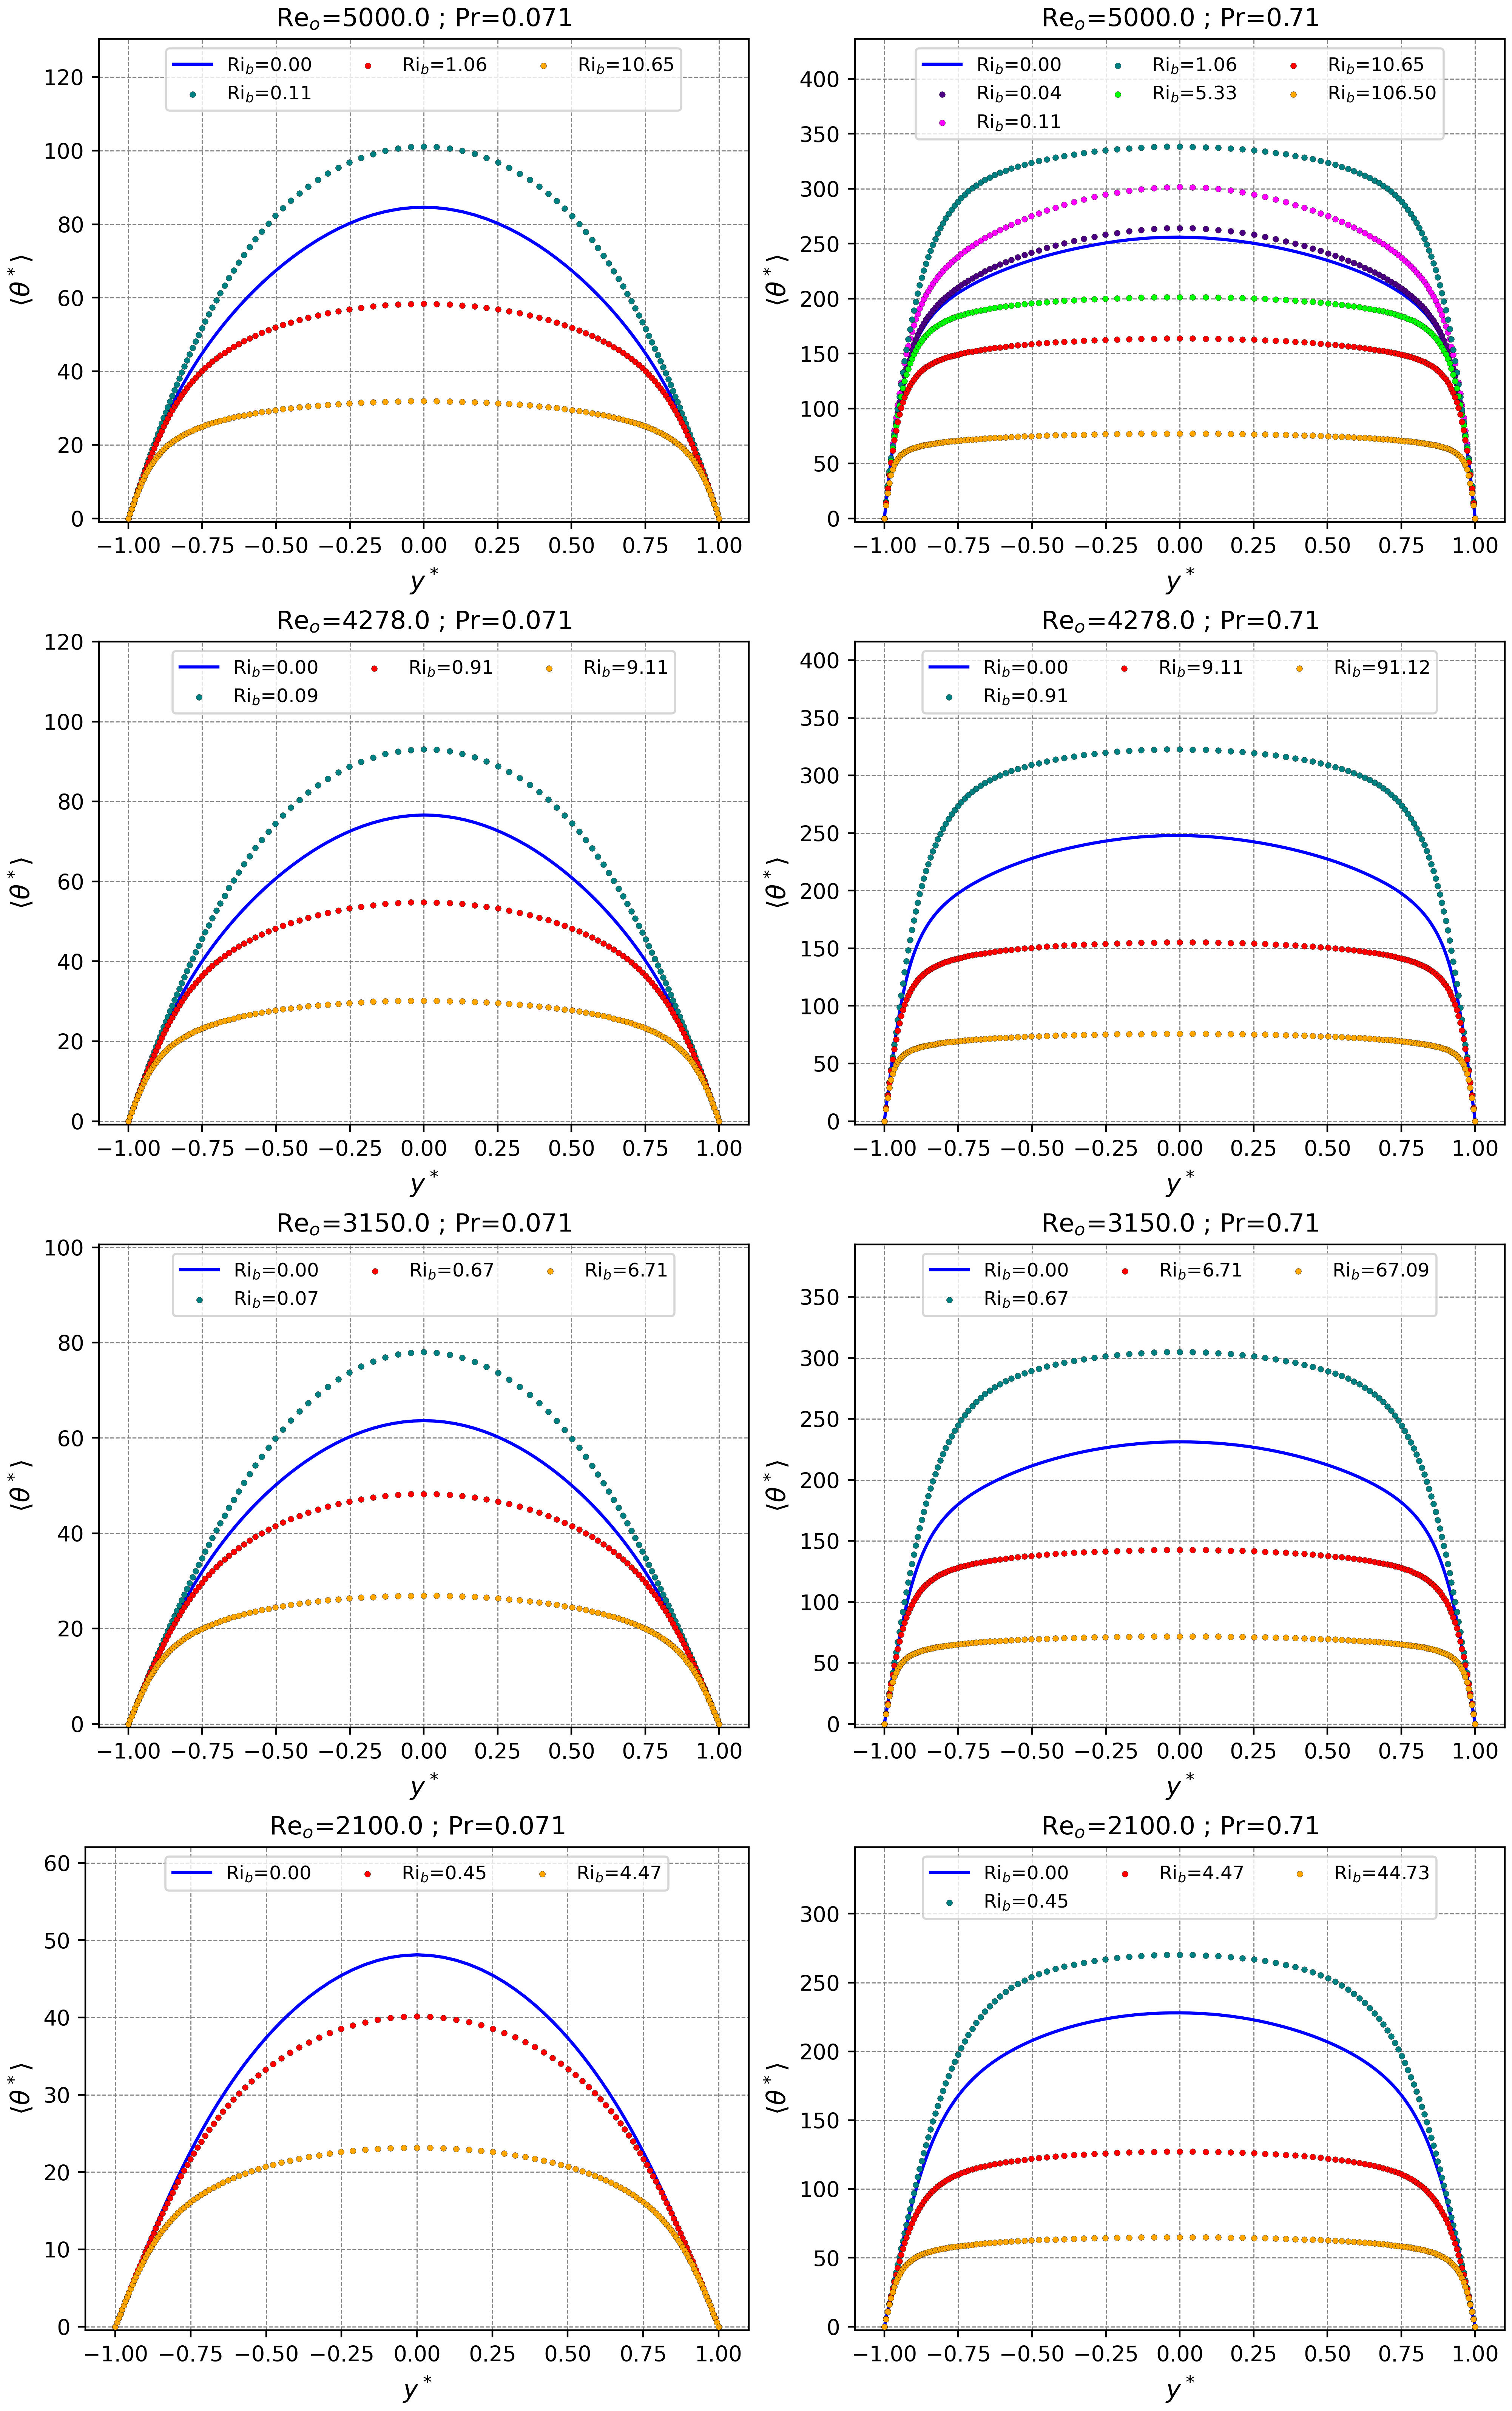
\includegraphics[width=0.9\textwidth]{figures/cap5/phi_tessel.png}  
%  \caption{}
%  \label{fig:tesselphi}
%\end{figure}
%
%\newpage
%
%\begin{figure}[H] % usa [H] solo si necesitas anclarla y tienes \usepackage{float}
%  \centering
%  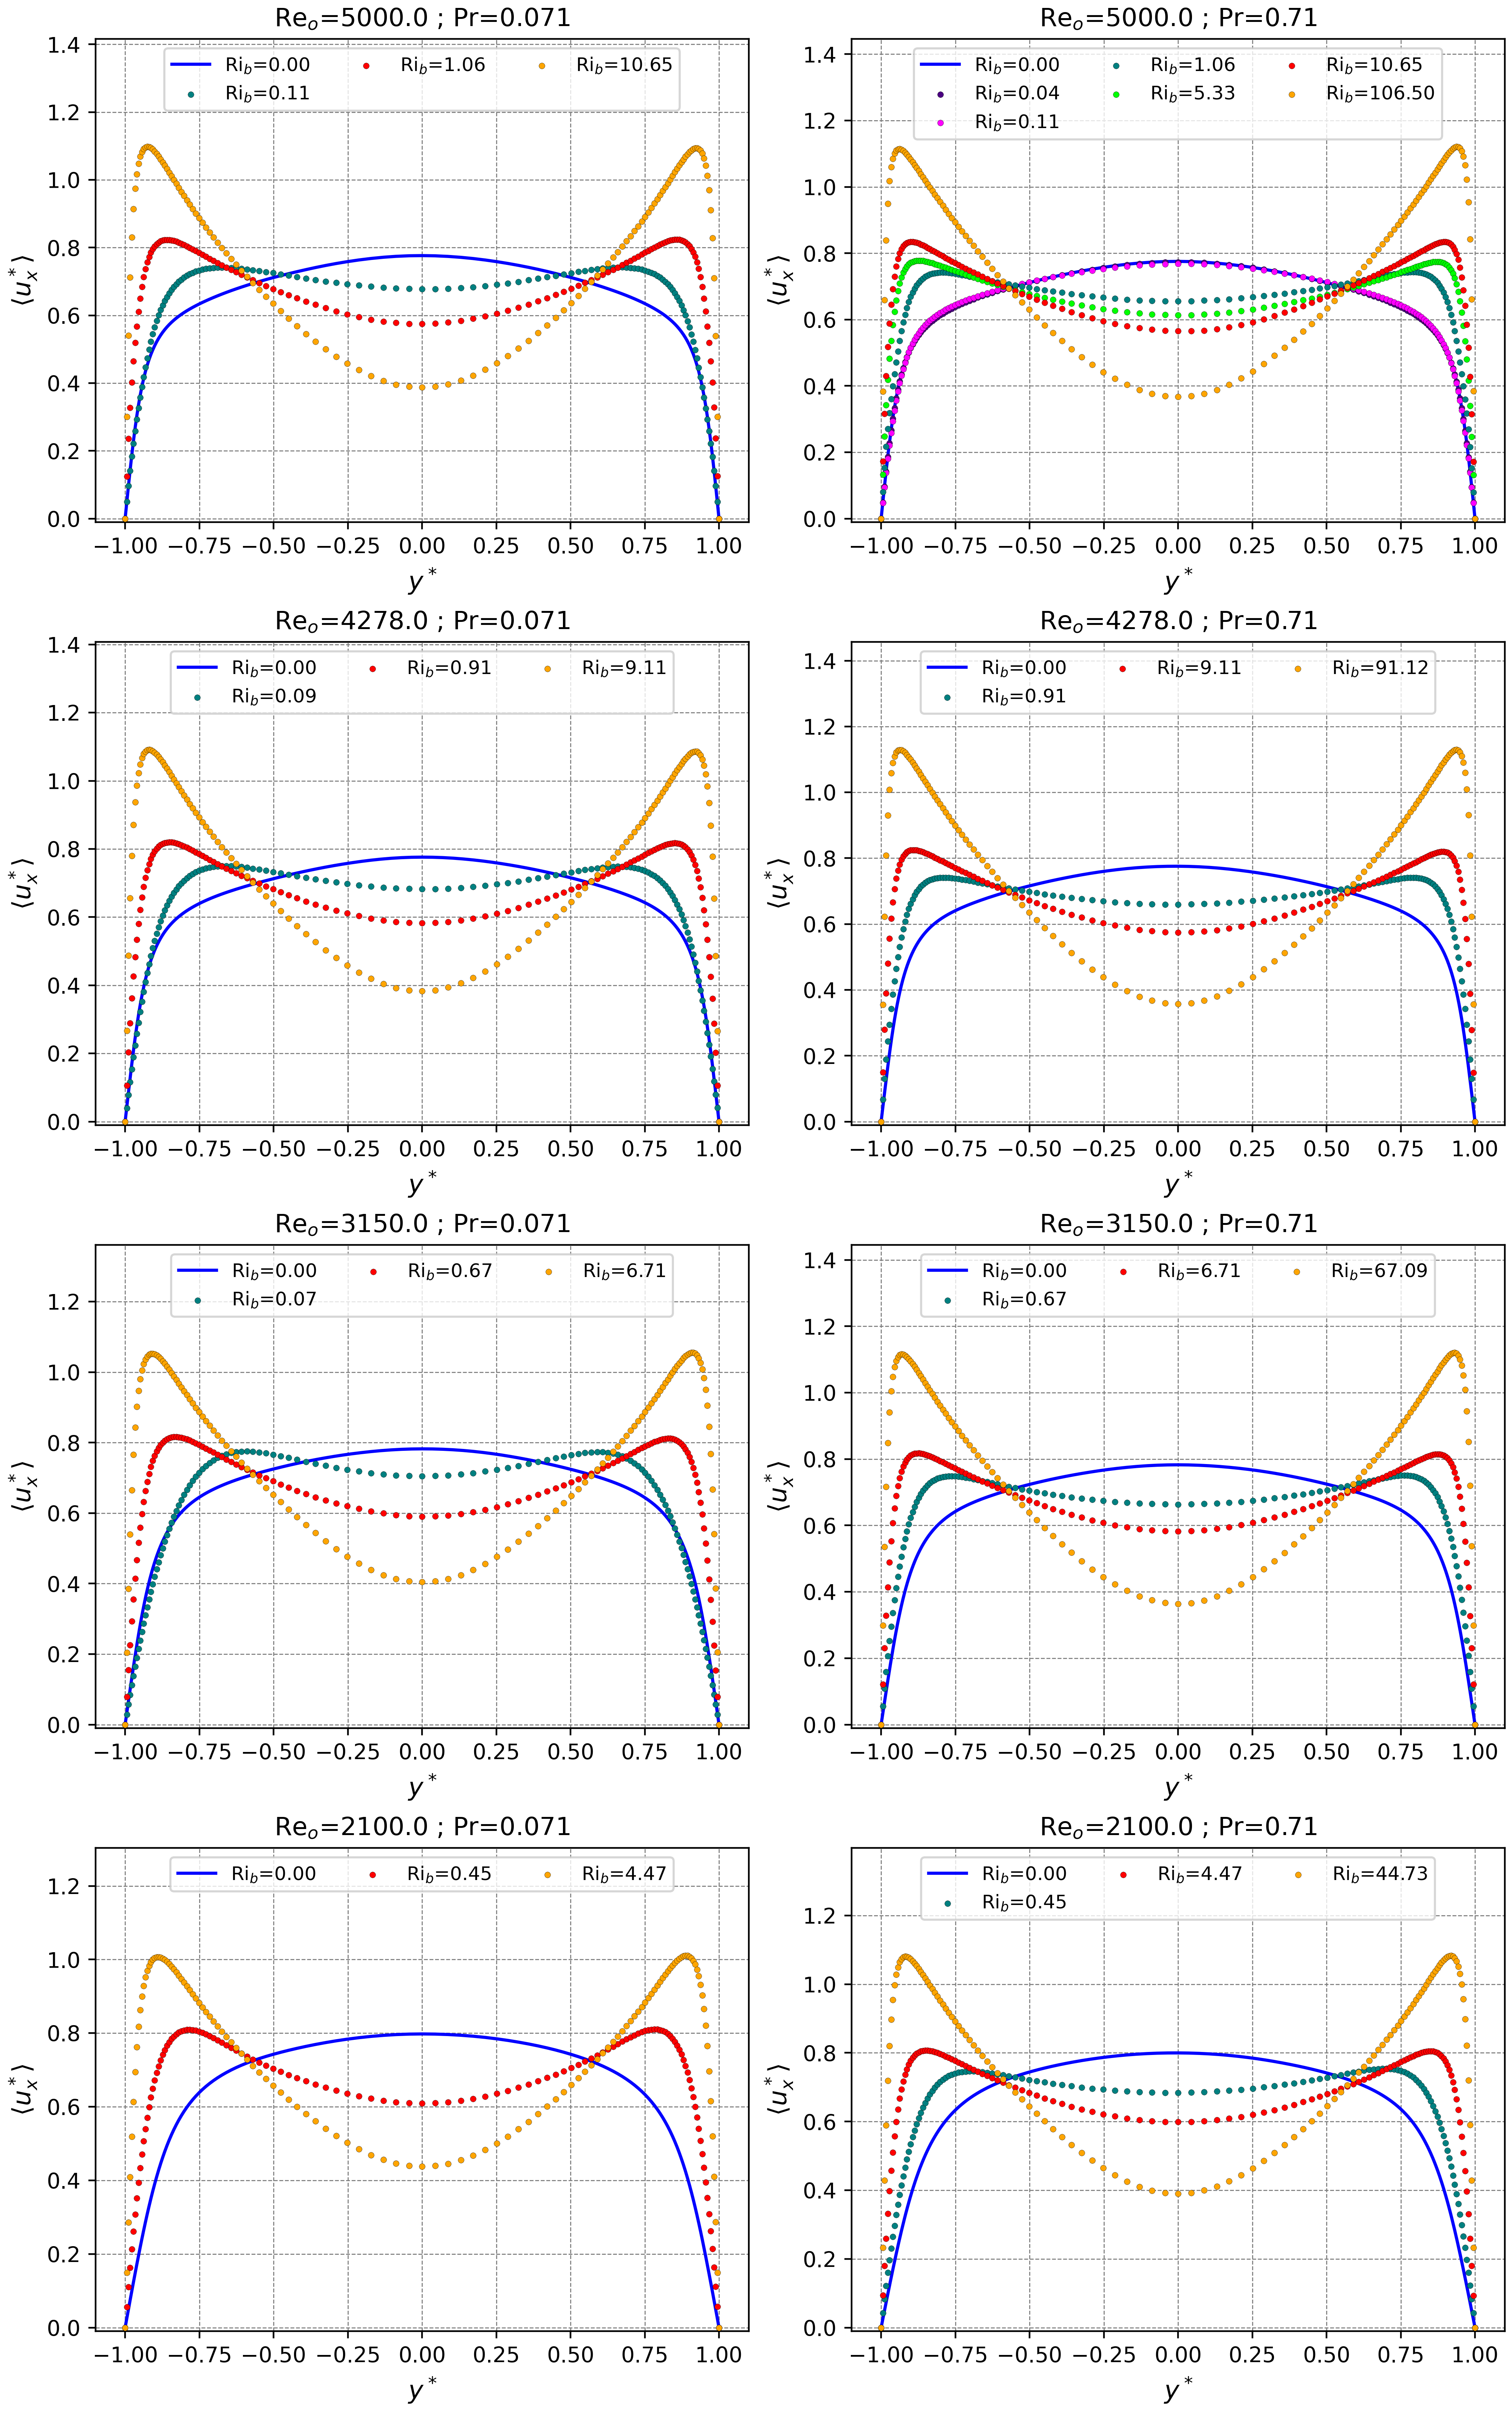
\includegraphics[width=0.9\textwidth]{figures/cap5/ux_tessel.png}  
%  \caption{}
%  \label{fig:tesselphi}
%\end{figure}

%################################################################################




\newpage
\subsection{Valores RMS de temperatura y velocidad} 

Las Figuras \ref{fig:rms-phi-Re5000-Pr071} y \ref{fig:rms-ux-Re5000-Pr071} muestran los perfiles de las fluctuaciones de temperatura adimensional y de velocidad \textit{streamwise}, respectivamente. Partiendo del caso puramente forzado, el incremento de la fuerza boyante provoca evoluciones distintas en los conjuntos \textbf{I} y \textbf{II} considerados anteriormente. En el primero, se observa una disminución (incremento) de las fluctuaciones de velocidad (temperatura) seguida de una ligera recuperación (leve descenso). En el segundo, las fluctuaciones de velocidad crecen de manera sostenida a medida que la fuerza boyante se intensifica, mientras que las de temperatura tienden a reducirse. Tendencias análogas han sido descritas por otros autores \cite{you2003direct,carr1973velocity}.

\begin{figure}[H]
  \centering
  \subfloat[]{
    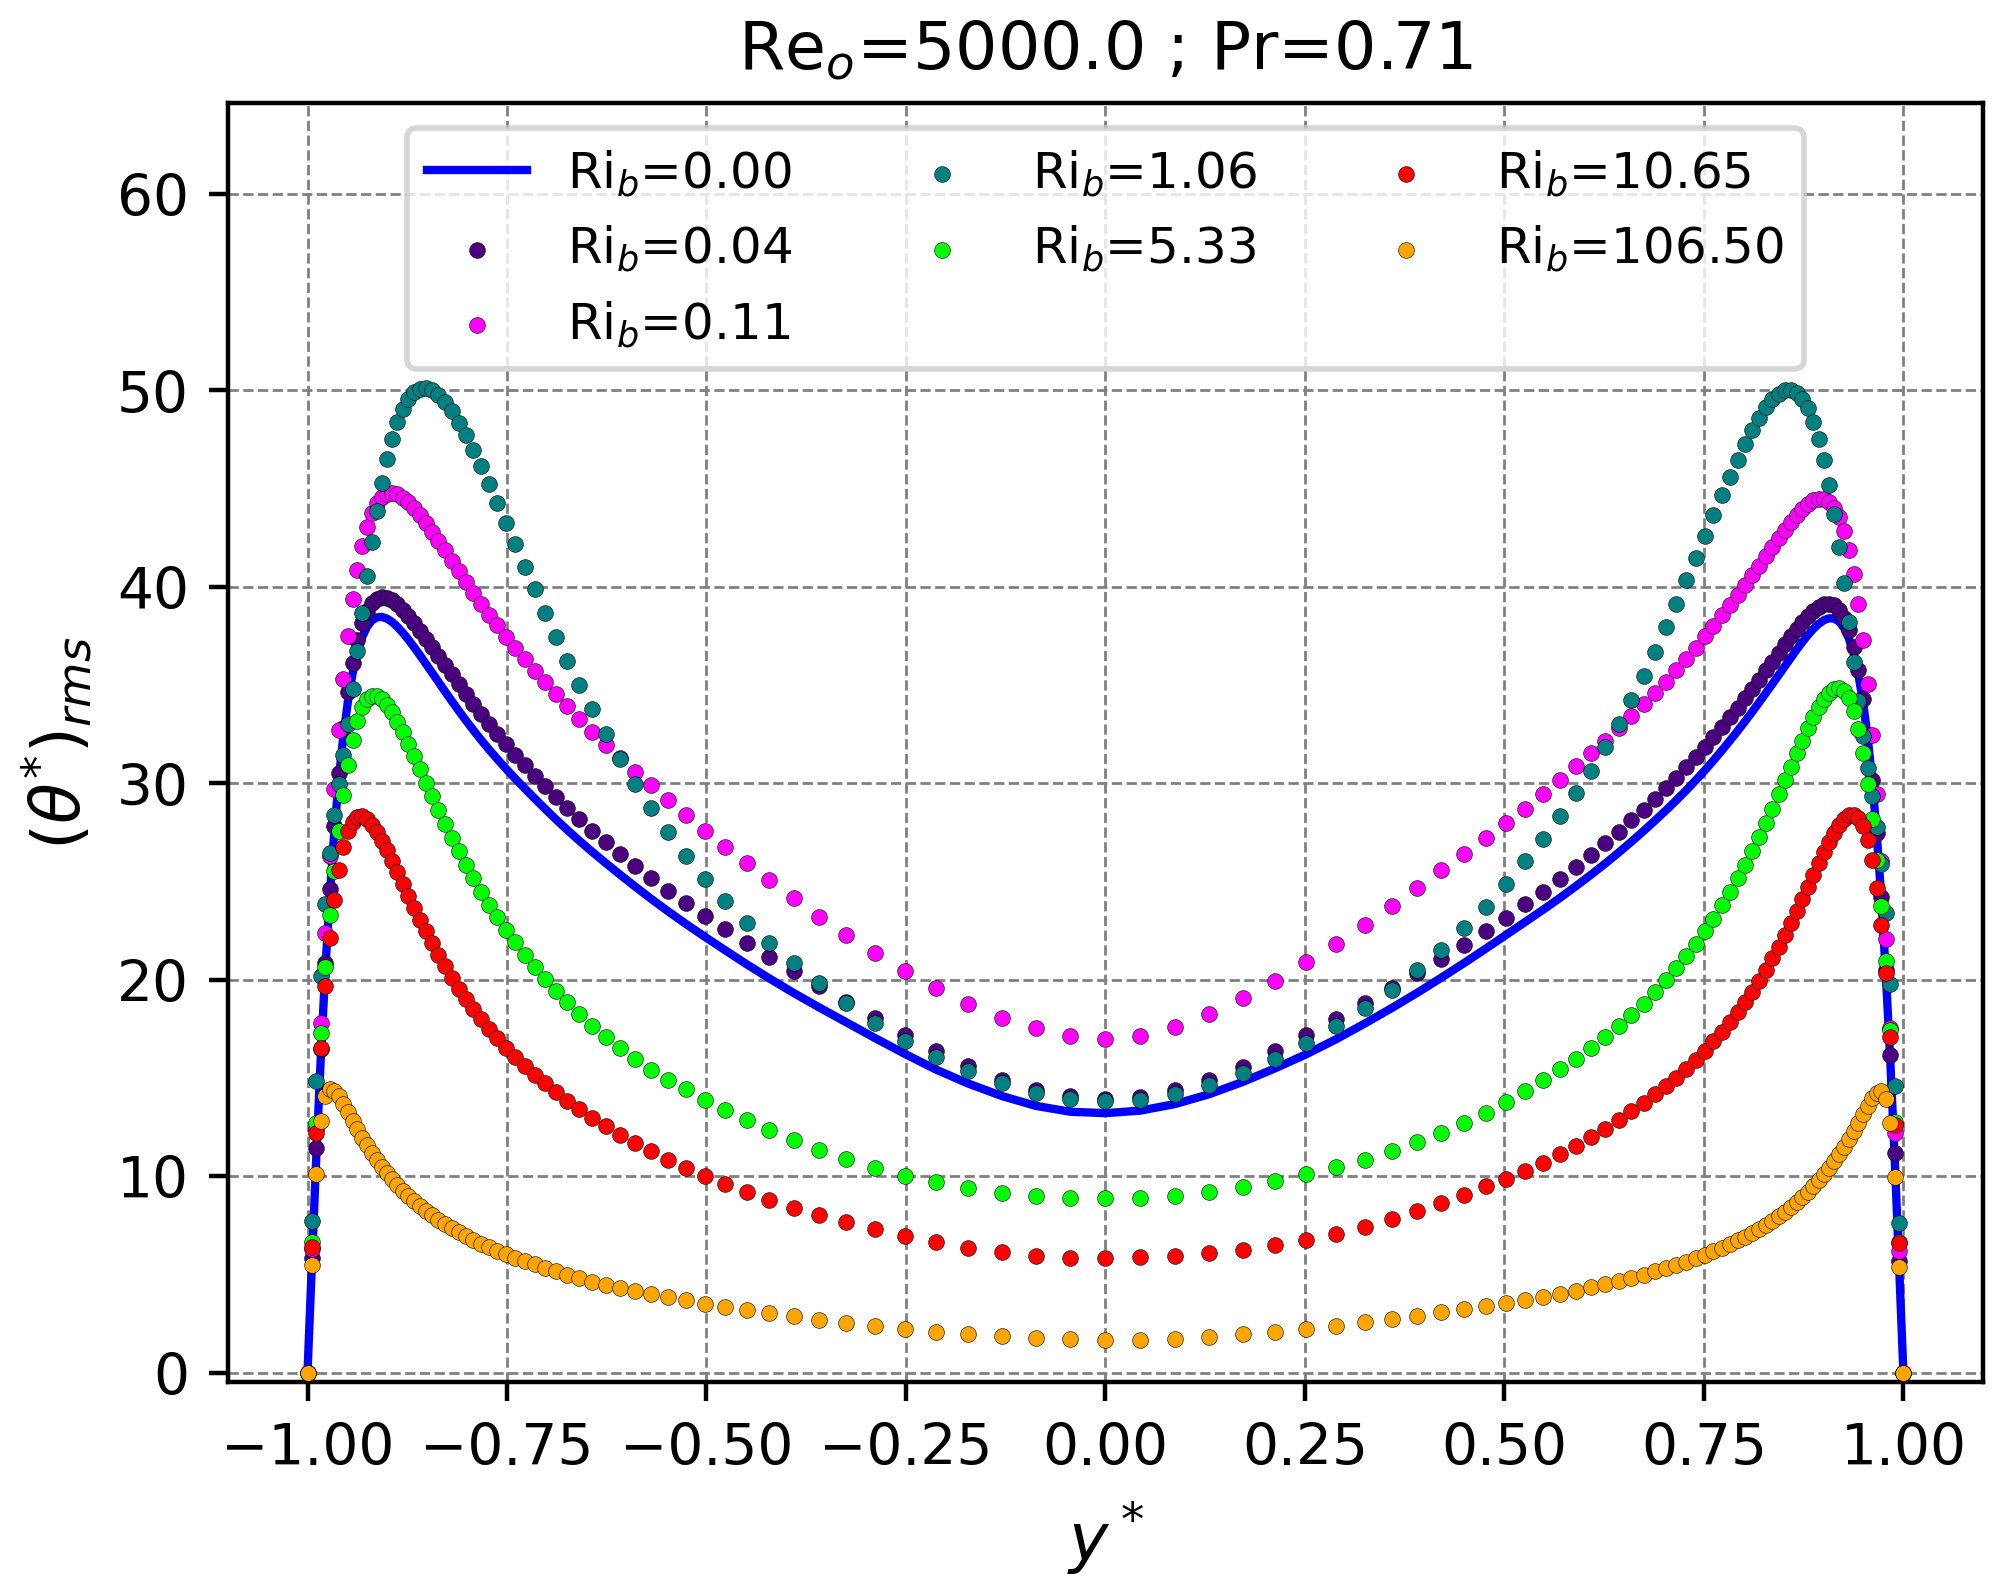
\includegraphics[width=0.49\textwidth]{figures/cap5/Re5000-Pr071/phi_rms_profile.png}
    \label{fig:rms-phi-Re5000-Pr071}}
  \subfloat[]{
    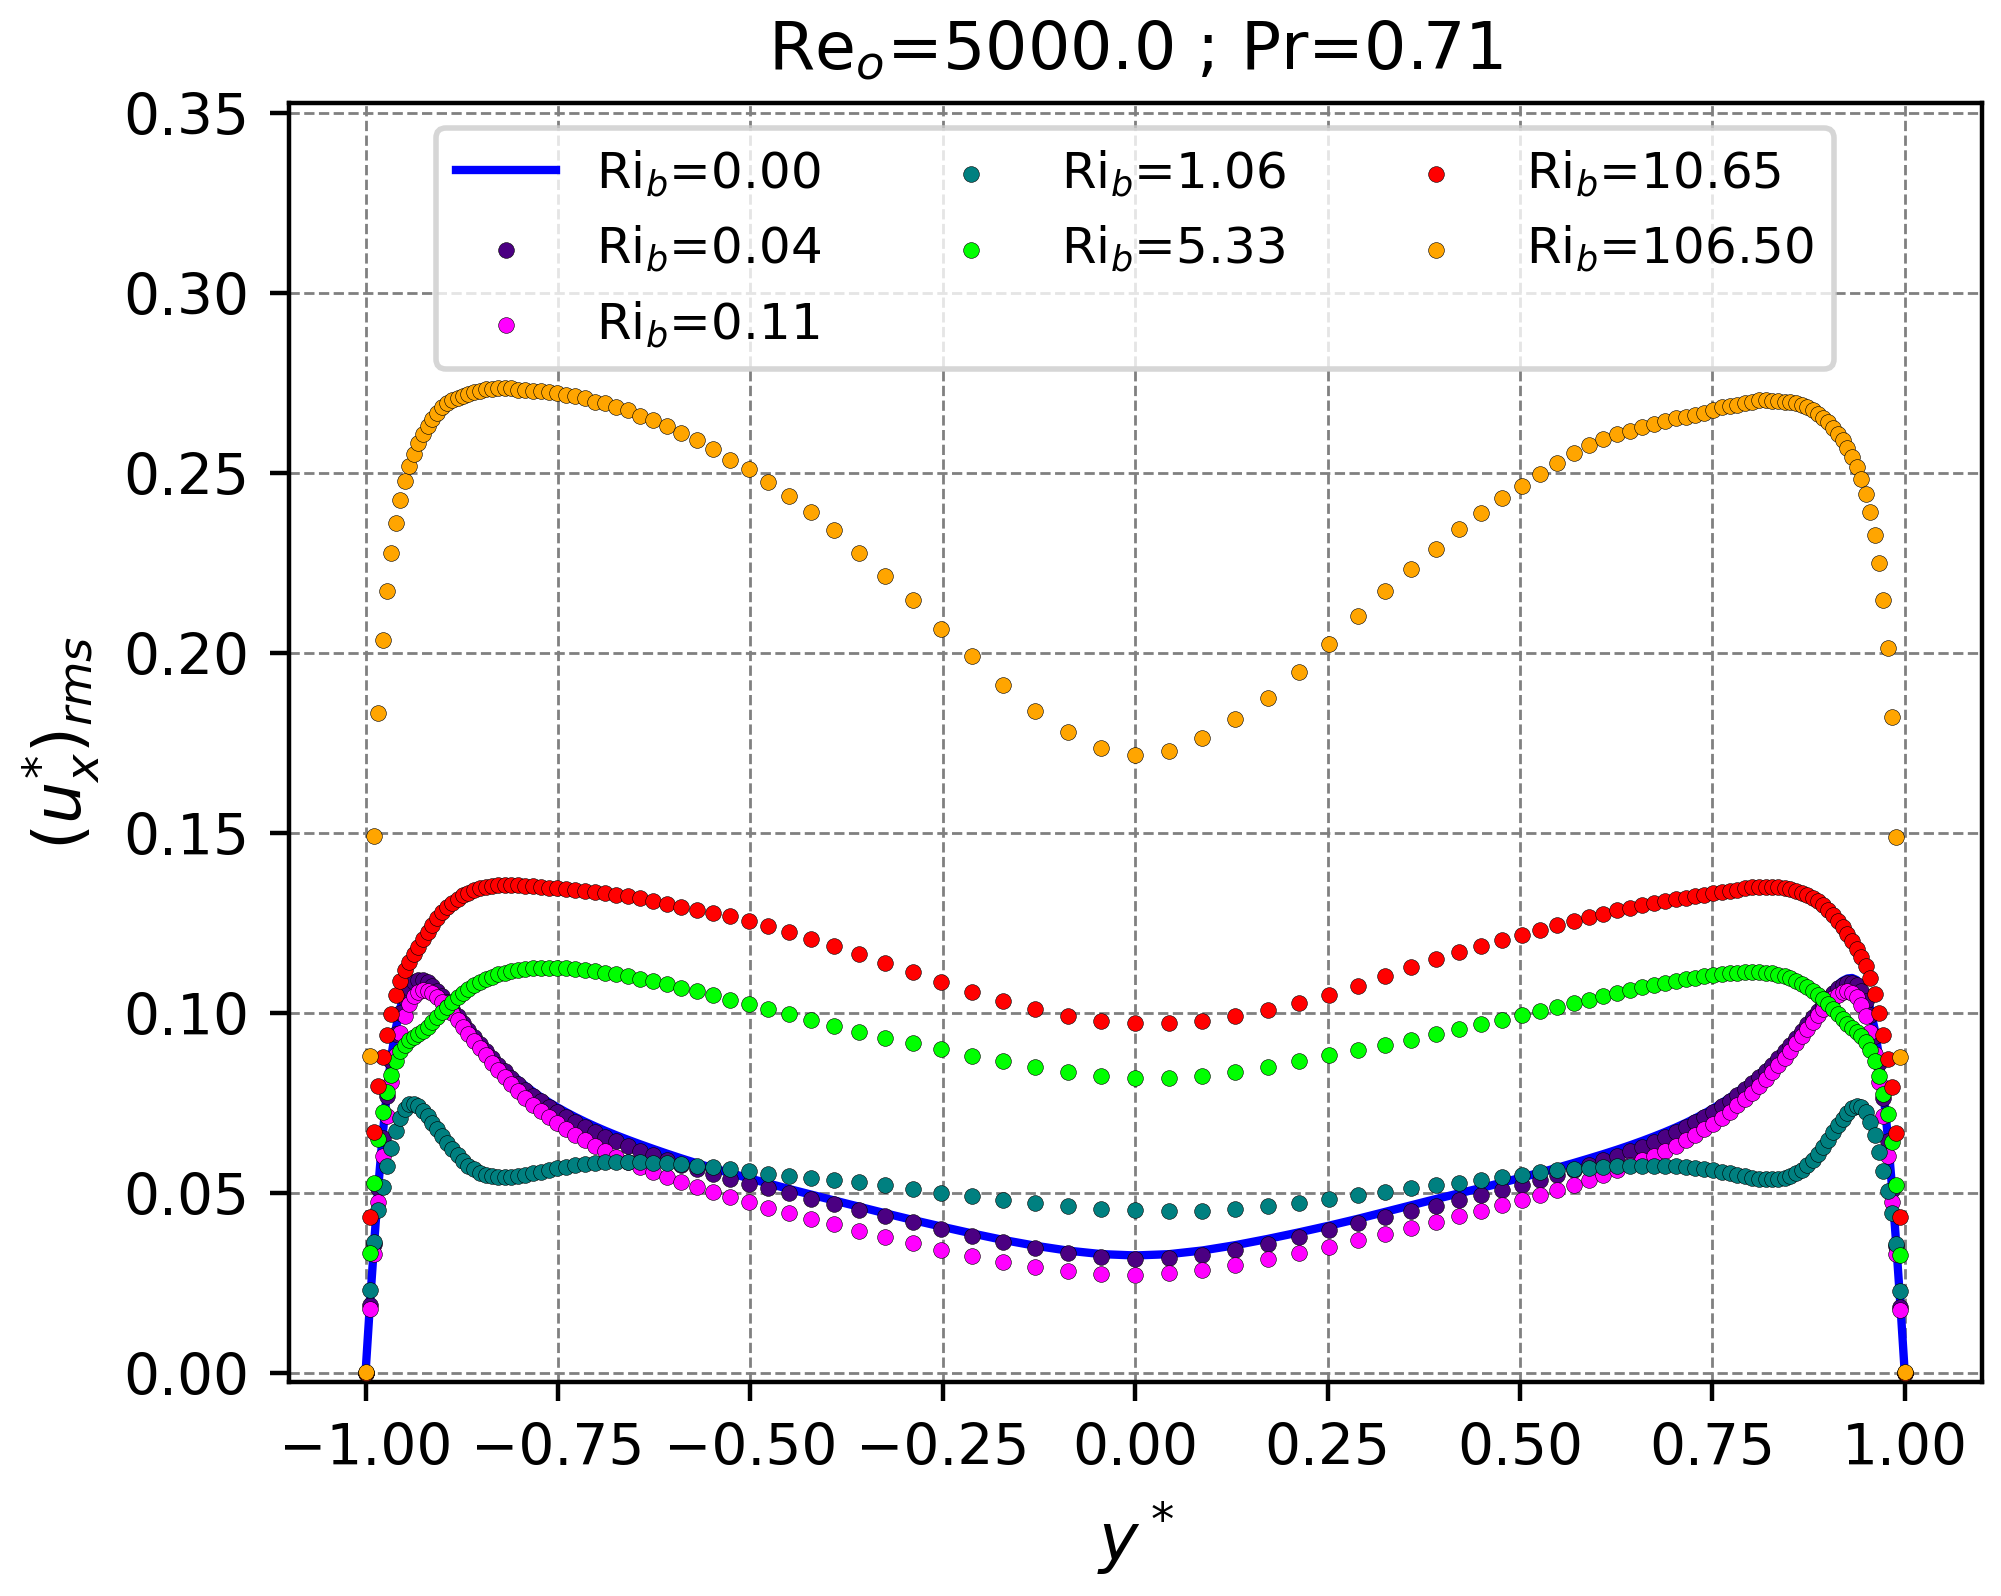
\includegraphics[width=0.49\textwidth]{figures/cap5/Re5000-Pr071/ux_rms_profile.png}
     \label{fig:rms-ux-Re5000-Pr071}}
    \caption{Fluctuaciones RMS: \textbf{(a)} velocidad en la dirección de la corriente y \textbf{(b)} temperatura adimensional.}
    \label{fig:rms-Re5000-Pr071}
\end{figure}

Como se aprecia en la Figura \ref{fig:rms-ux-Re5000-Pr071}, la aparicion de la fuerza boyante de baja intensidad realtiva produce primero una leve estabilización del flujo, evidenciada por una disminución de aproximadamente un 40$\%$ en los máximos de $(u^*_x)_{rms}$ próximos a las paredes. En contraste, las fluctuaciones de temperatura $T$ aumentan debido al incremento del flujo de calor impuesto y sus máximos se desplazan hacia el centro del canal, favorecidos por una relativa y débil redistribución causada por la turbulencia. Para Ri$_b$=5.33 la fuerza boyante adquiere mayor preponderancia y las fluctuaciones de velocidad crecen en todo el ancho del canal; por ejemplo, en el caso de Ri$_b$=10.65 el valor en el centro es un 100$\%$ mayor respecto al caso con Ri$_b$=1.06. Este incremento de la agitación dinámica redistribuye las fluctuaciones de temperatura, que disminuyen la magnitud adimensional respecto al caso de convección forzada (Figura \ref{fig:rms-phi-Re5000-Pr071}).

\subsection{Flujos turbulentos de calor} 

En la Figura \ref{fig:uxphi_f-Re5000-Pr071} se expone el perfil de la correlación $\langle u_x^{\ast \prime } \theta^{\ast \prime } \rangle$. Esta cantidad corresponde al flujo de calor turbulento \textit{streamwise} que surge como consecuencia de promediar la ecuación de conservación de energía \cite{kundu,pope2001turbulent}, y puede interpretarse como el calor transportado por las estructuras producidas por el flujo turbulento. 

\begin{figure}[H]
  \centering
  \subfloat[]{
    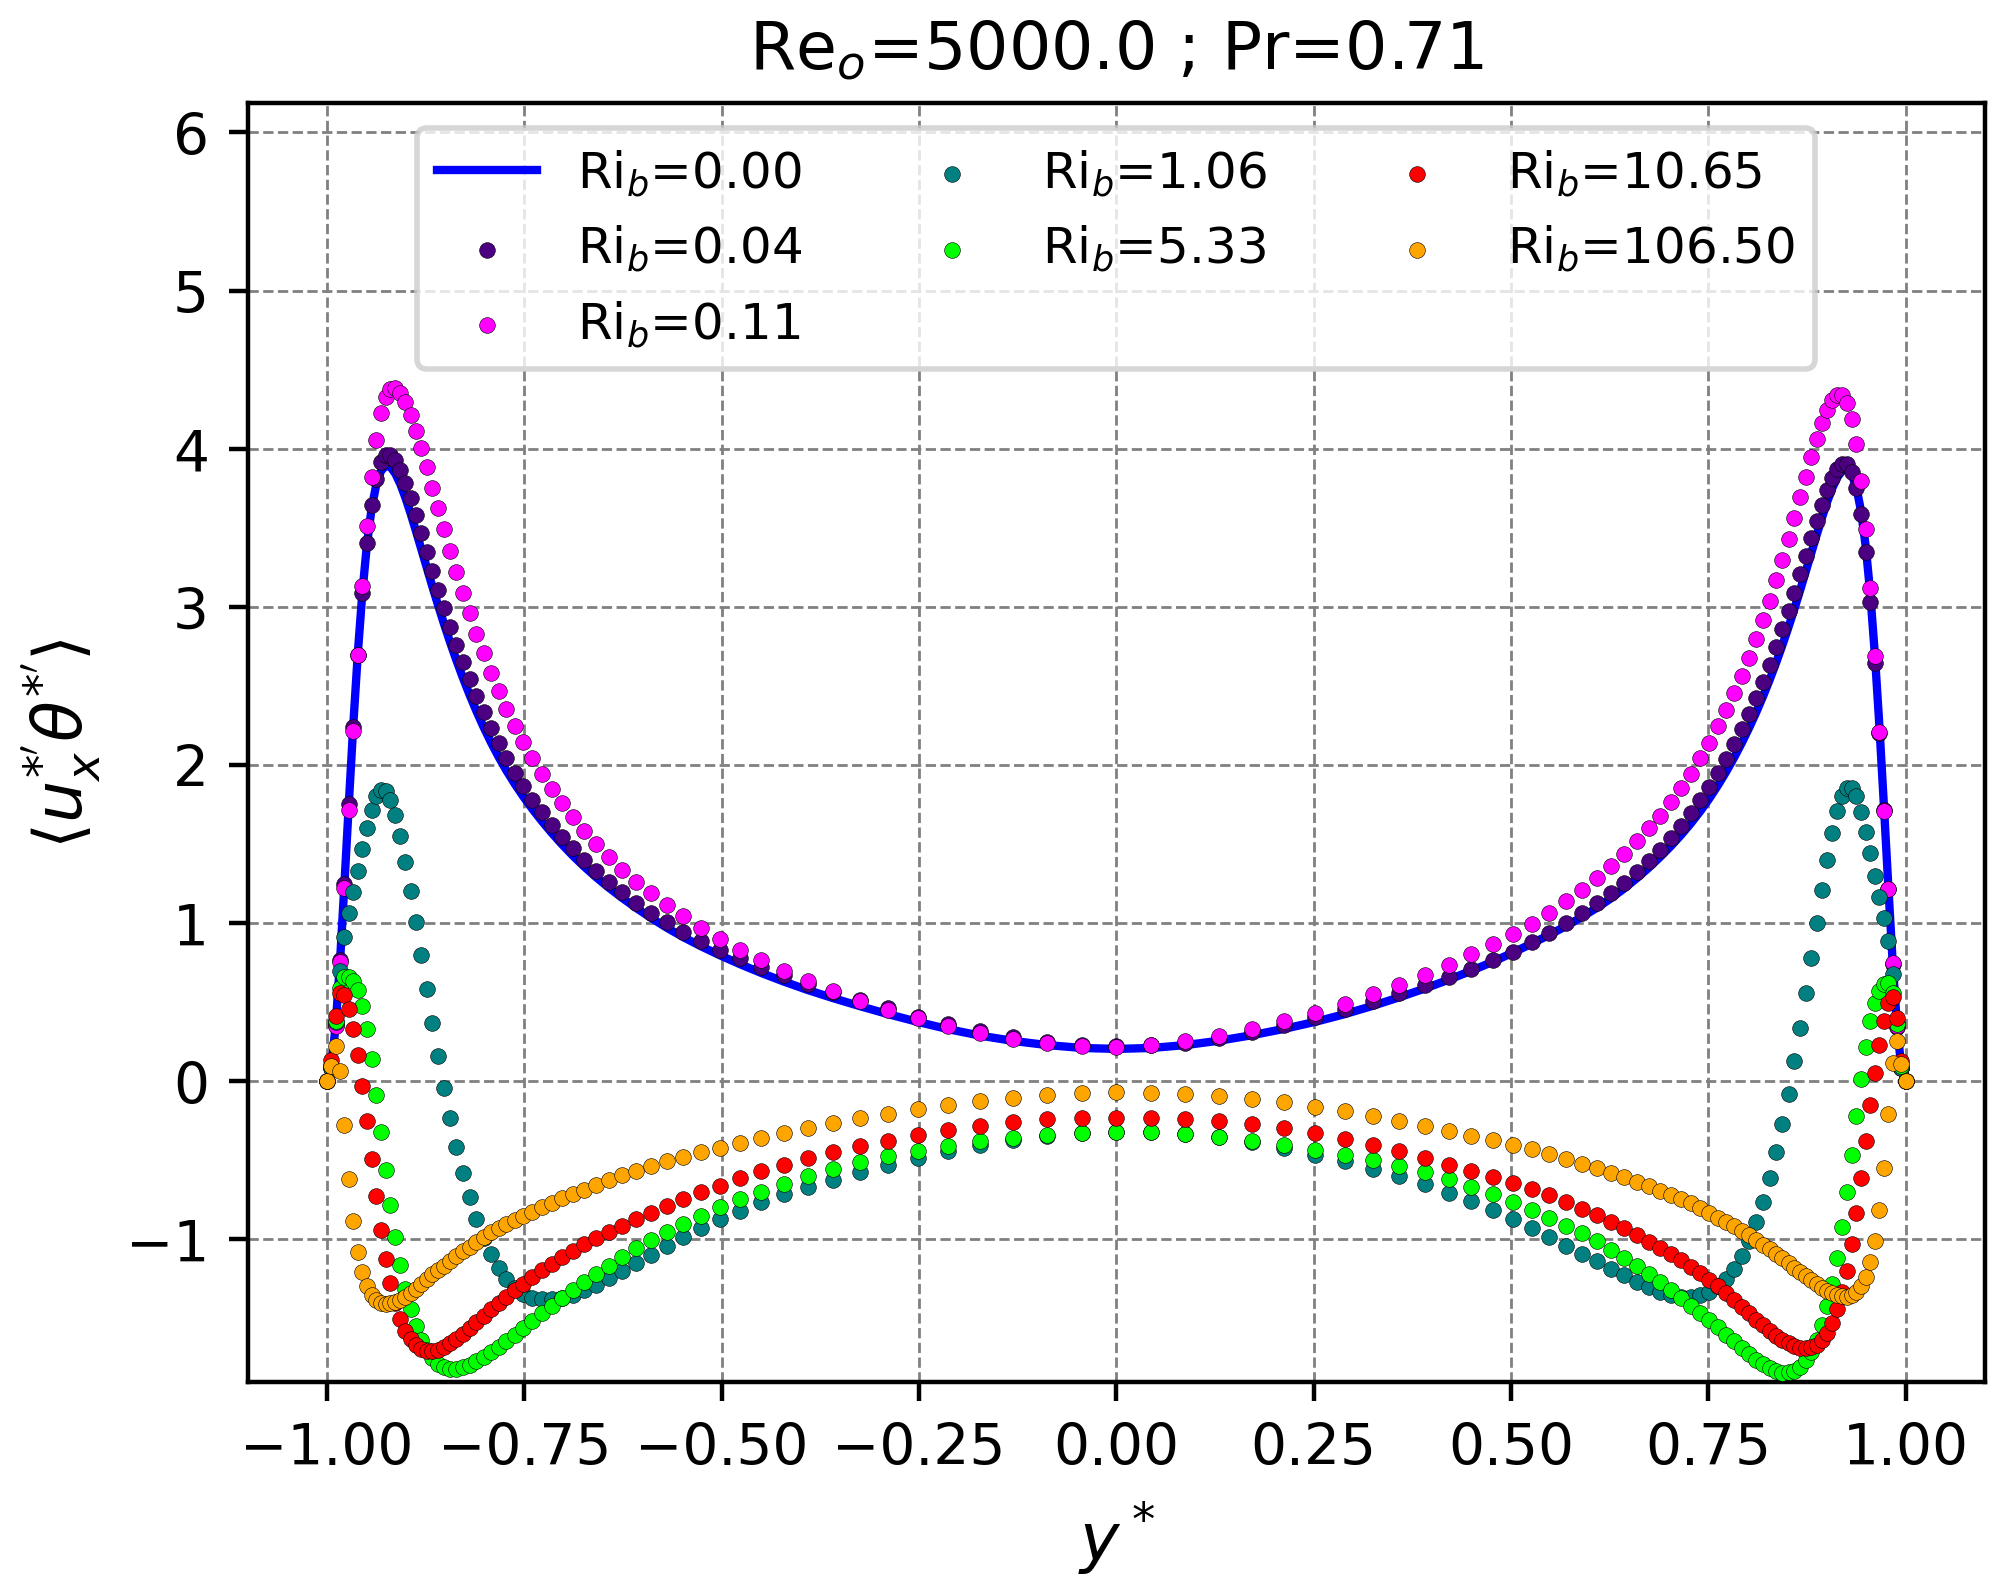
\includegraphics[width=0.53\textwidth]{figures/cap5/Re5000-Pr071/uxphif_profile.png}
    \label{fig:uxphi_f-Re5000-Pr071}}
  \subfloat[]{
    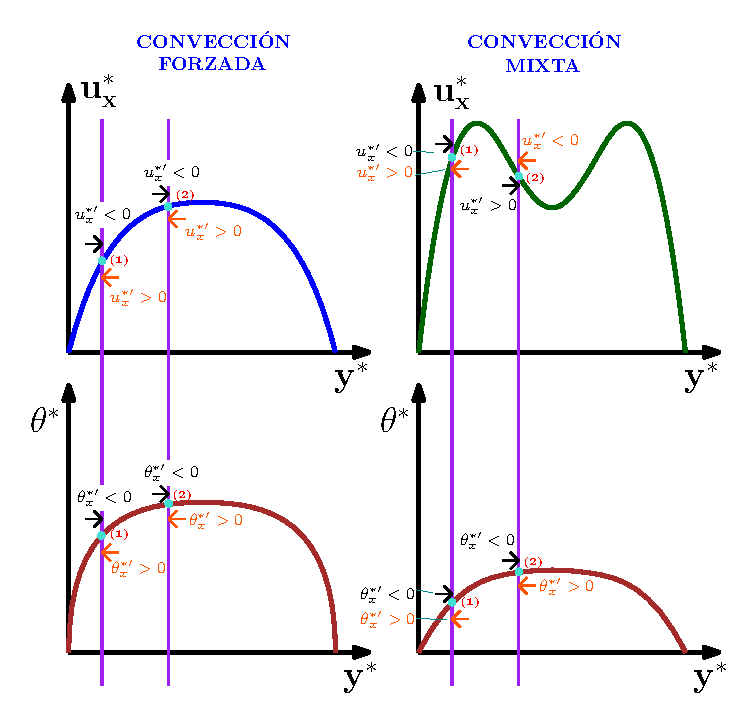
\includegraphics[width=0.46\textwidth]{figures/cap5/Re5000-Pr071/uxphif_esquema.eps}
     \label{fig:uxphi_esquema-Re5000-Pr071}}
    \caption{\textbf{(a)} Flujo de calor turbulento en la dirección de la corriente. \textbf{(b)} Esquemá de perfiles de temperatura y velocidad para convección forzada y mixta.}
    \label{fig:rms-Re5000-Pr071}
\end{figure}

En el seno del canal se aprecia una diferencia marcada entre el caso forzado y aquellos muy próximos a este (Ri$_b$=0.04,0.11), y el resto de casos. Esta disparidad se puede entender cualitativamente a traves de los perfiles de $u^*_x$ y $\theta^*$. Para ello, en la Figura \ref{fig:uxphi_esquema-Re5000-Pr071} se muestran los perfiles esquemáticos de ambas magnitudes para los regímenes de conveción forzada y mixta:

\begin{itemize}

\item \textbf{Cerca la pared:} analizando el caso forzado, si una partícula de fluido próxima a la pared (punto \textbf{(1)}) se desplaza un diferencial $dy^*$ a la izquierda, produce una fluctuación negativa en la velocidad ($u^{* \prime}_x <0$), esto ocasiona que la misma se traslade de una zona más fría a una más caliente, y por lo tanto, experimenta una fluctuación negativa en su temperatura adimensional ($\theta^{* \prime}<0$) que se traduce en una correlación positiva $\langle u_x^{\ast \prime } \theta^{\ast \prime } \rangle > 0$. 

Por otro lado, si la partícula de fluido se desplaza un diferencial $dy^*$ a la derecha, esto genera una fluctuación positiva en la velocidad ($u^{* \prime}_x >0$) y la misma se desplaza de una región más caliente a una más fría, y en consecuencia $\theta^{* \prime}$ es positiva y se produce nuevamente una correlación positiva.

La situación es completamente análoga para el caso de convección mixta.

\item \textbf{Cerca del centro del canal:} En el caso de convección forzada la situación es idéntica: un desplazamiento $dy^*$ a la izquierda (derecha) desde una región cercana al centro (punto \textbf{(2)}) da lugar a una fluctuación negativa (positiva) de la velocidad y la partícula se traslada de una región más fría (caliente) a una más caliente (fría) y nuevamente la correlación resulta postiva. Por cuál, en el caso forzado se tiene una correlación positiva global. 

Sin embargo, si uno realiza el mismo análisis para el caso de convección mixta, ocurre lo contrario, en otras palabras, un desplazamiento $dy^*$ a la izquierda (derecha) produce una fluctuación positiva (negativa) de la velocidad y la partícula se traslada de una región más fría (caliente) a una más caliente (fría) dado como resultado una fluctuación negativa de la temperatura adimensional en ambas situaciones y por lo tanto, en el seno del canal, la correlación $\langle u_x^{\ast \prime } \theta^{\ast \prime } \rangle$ es negativa.
\end{itemize}  

A partir del análisis anterior, se puede afirmar, que la disparidad del comportamiento  entre ambos regímenes de convección es consecuencia del cambio de la concavidad del perfil de velocidad en el seno del canal, debido al aumento de la fuerza boyante.


\begin{figure}[H] % usa [H] solo si necesitas anclarla y tienes \usepackage{float}
  \centering
  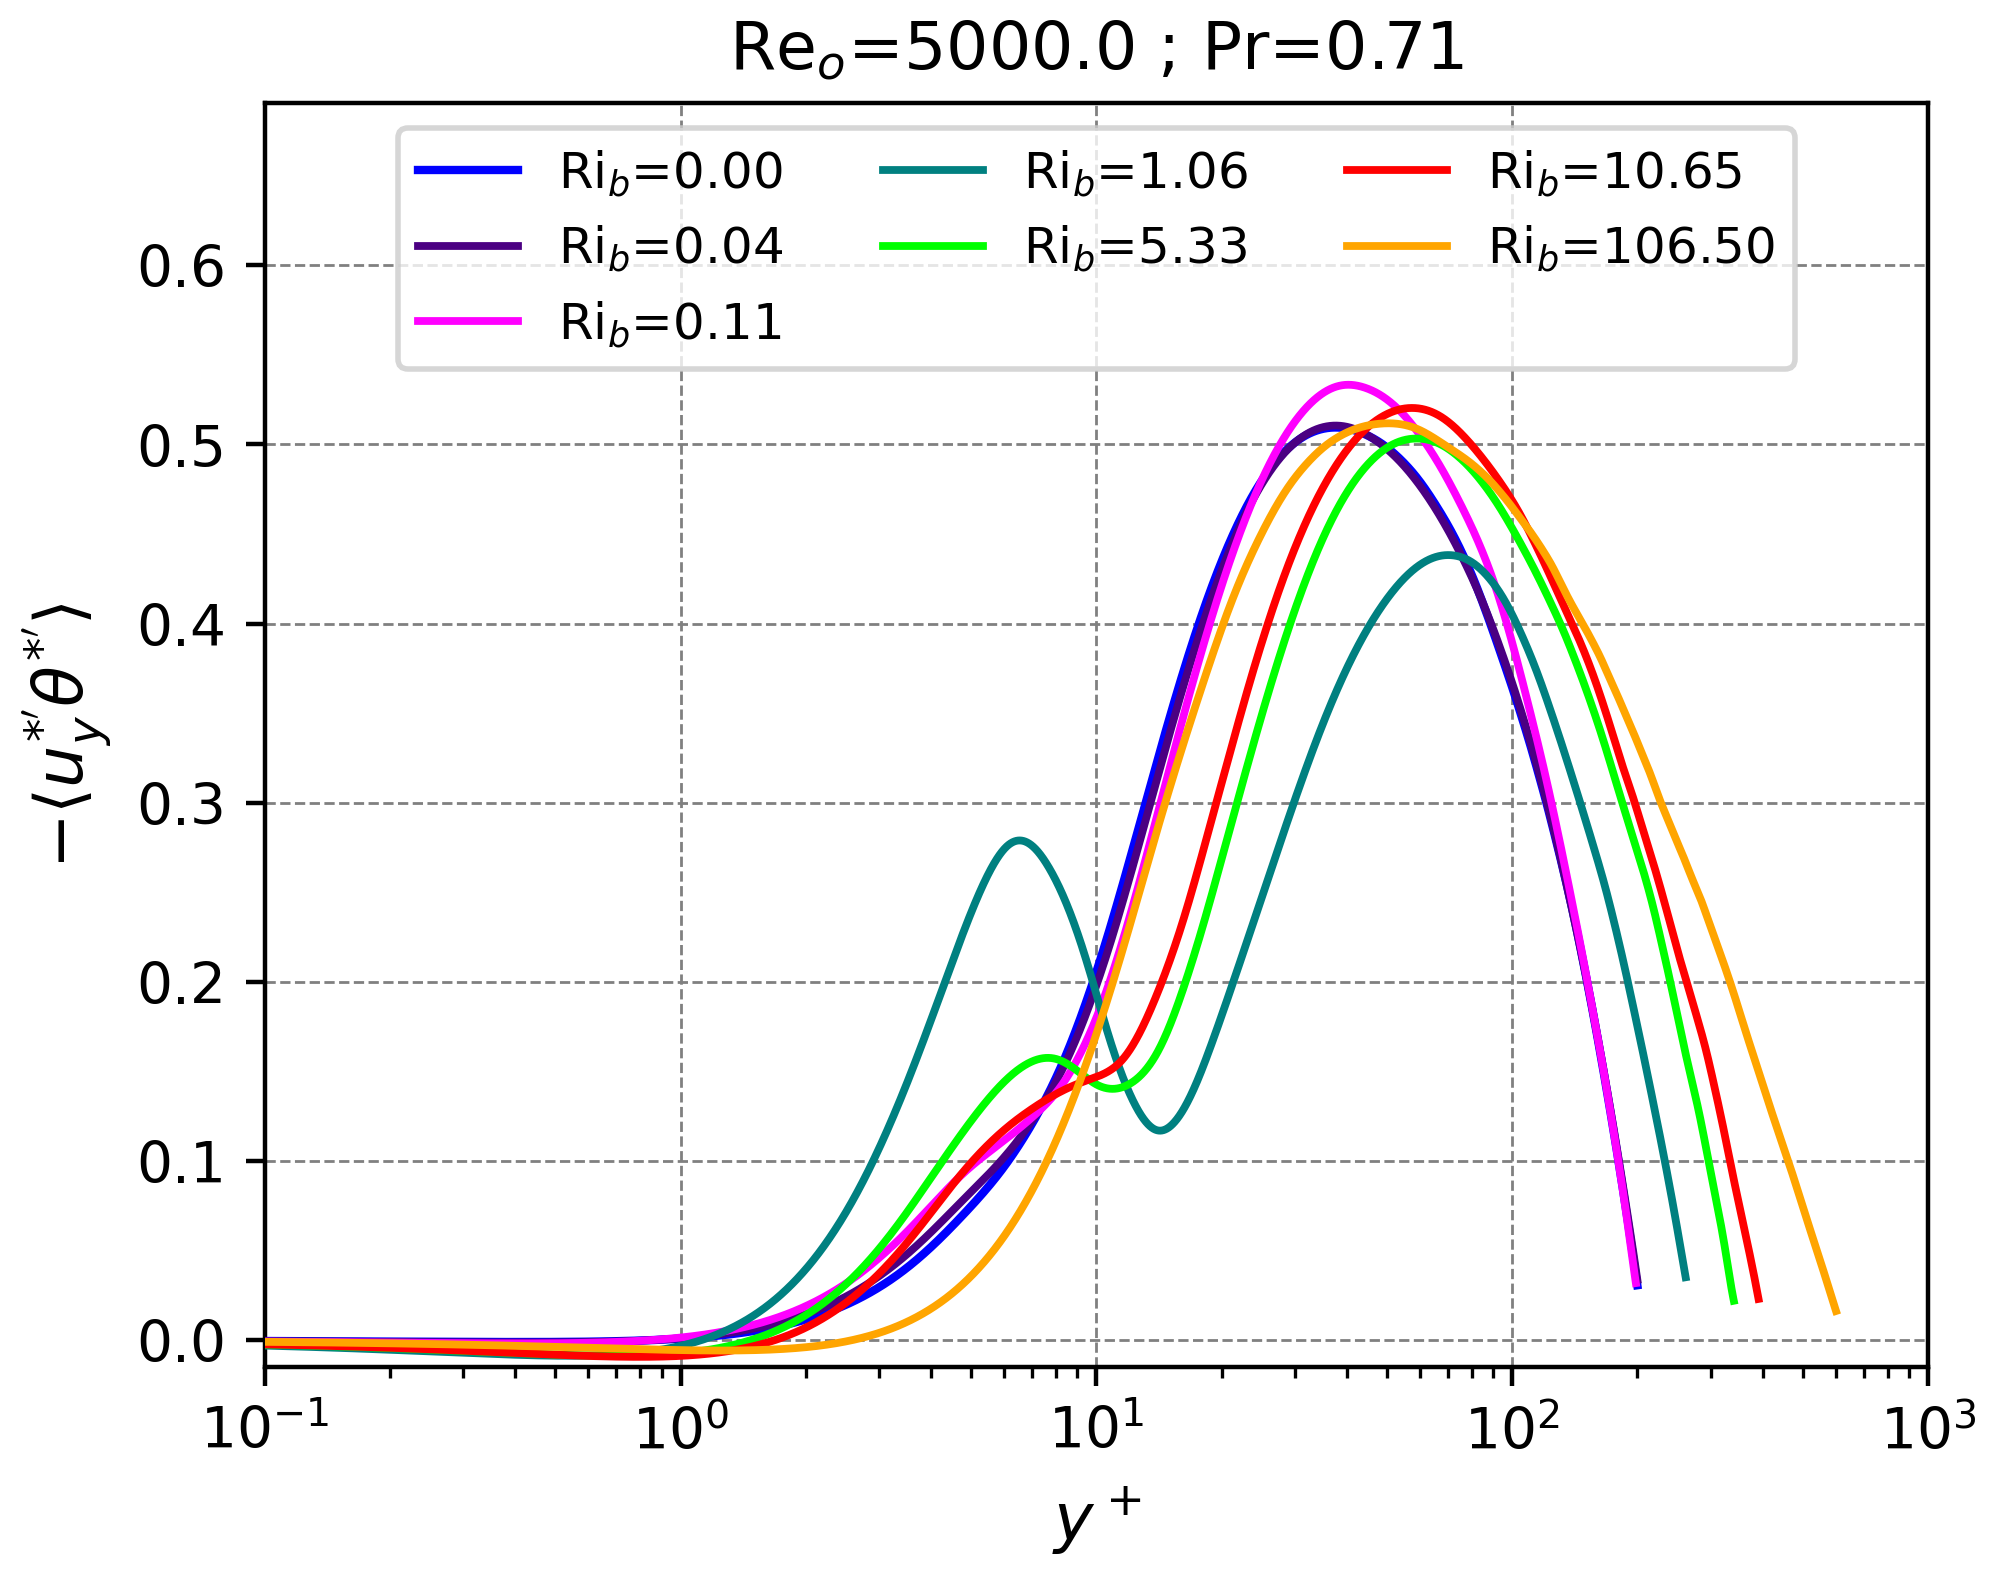
\includegraphics[width=0.9\textwidth]{figures/cap5/Re5000-Pr071/uyphif_profile.png}  
  \caption{Flujo de calor turbulento en la dirección normal a la pared.}
  \label{fig:uyphi_f-Re5000-Pr071}
\end{figure}

Por último, en la Figura \ref{fig:uyphi_f-Re5000-Pr071} se expone el perfil de la correlación $\langle u_y^{\ast \prime } \theta^{\ast \prime } \rangle$. 

Ri_b = 0.04,0.11,1.06 etc se observa un corrimiento del maximo cerca de la pared hacia el seno del canal


\section{Comparación entre casos de distinto Prandtl}

%En esta sección se compara los casos con Re$_o$=5000 y Pr=0.071,0.71. La Figura \ref{fig:plus-ux-Re5000-Prs} presenta lo perfiles de velocidad media en términos de \textit{wall units}. En la subcapa viscosa ($y^+ < 5$), es posible aproximar la velocidad como $\langle u_x^+ \rangle \simeq y^+ + \mathcal{O}((y^+)^2)$ \cite{pope2001turbulent}, cuya dicha aproximación está representada con la linea negra del gráfico. En esta región, el tensor de esfuerzo de Reynolds es despreciable comparado con el tensor de esfuerzo viscoso. En efecto, se puede apreciar que independientemente de la sustancia y de fuerza boyante, todos los casos muestran ser consistentes con dicha aproximación.

En esta sección se comparan los casos con $Re_o$ = 5000 y Pr = 0.071 y 0.71. La Figura \ref{fig:plus-ux-Re5000-Prs} muestra los perfiles de velocidad media expresados en unidades de pared (\textit{wall units}). En la subcapa viscosa ($y^+ < 5$) la velocidad puede aproximarse por
$$\langle u_x^+ \rangle \;\simeq\; y^+ + \mathcal{O} \left[(y^+)^{2} \right],$$
según Pope \cite{pope2001turbulent}. Esta ley se indica en la figura con la línea negra de referencia. En dicha región las tensiones de Reynolds son despreciables frente a las tensiones viscosas, de modo que el perfil depende casi exclusivamente de la distancia normalizada a la pared. Como puede verse, todos los casos, independientemente del número de Prandtl y de la fuerza boyante, siguen de cerca esta aproximación lineal, lo que confirma la validez de la ley en la subcapa viscosa. 

Por otra parte, en la región logarítmica (\textit{log-law region}), en condiciones de convección forzada, la velocidad media en la dirección de la corriente se alinea perfectamente con la ley logarítmica clásica \cite{kawamura2000dns}. Sin embargo, esta ley ya no es válida al considerar la flotabilidad \cite{zhou2024direct}. 

\begin{figure}[H]
  \centering
    \subfloat[]{
    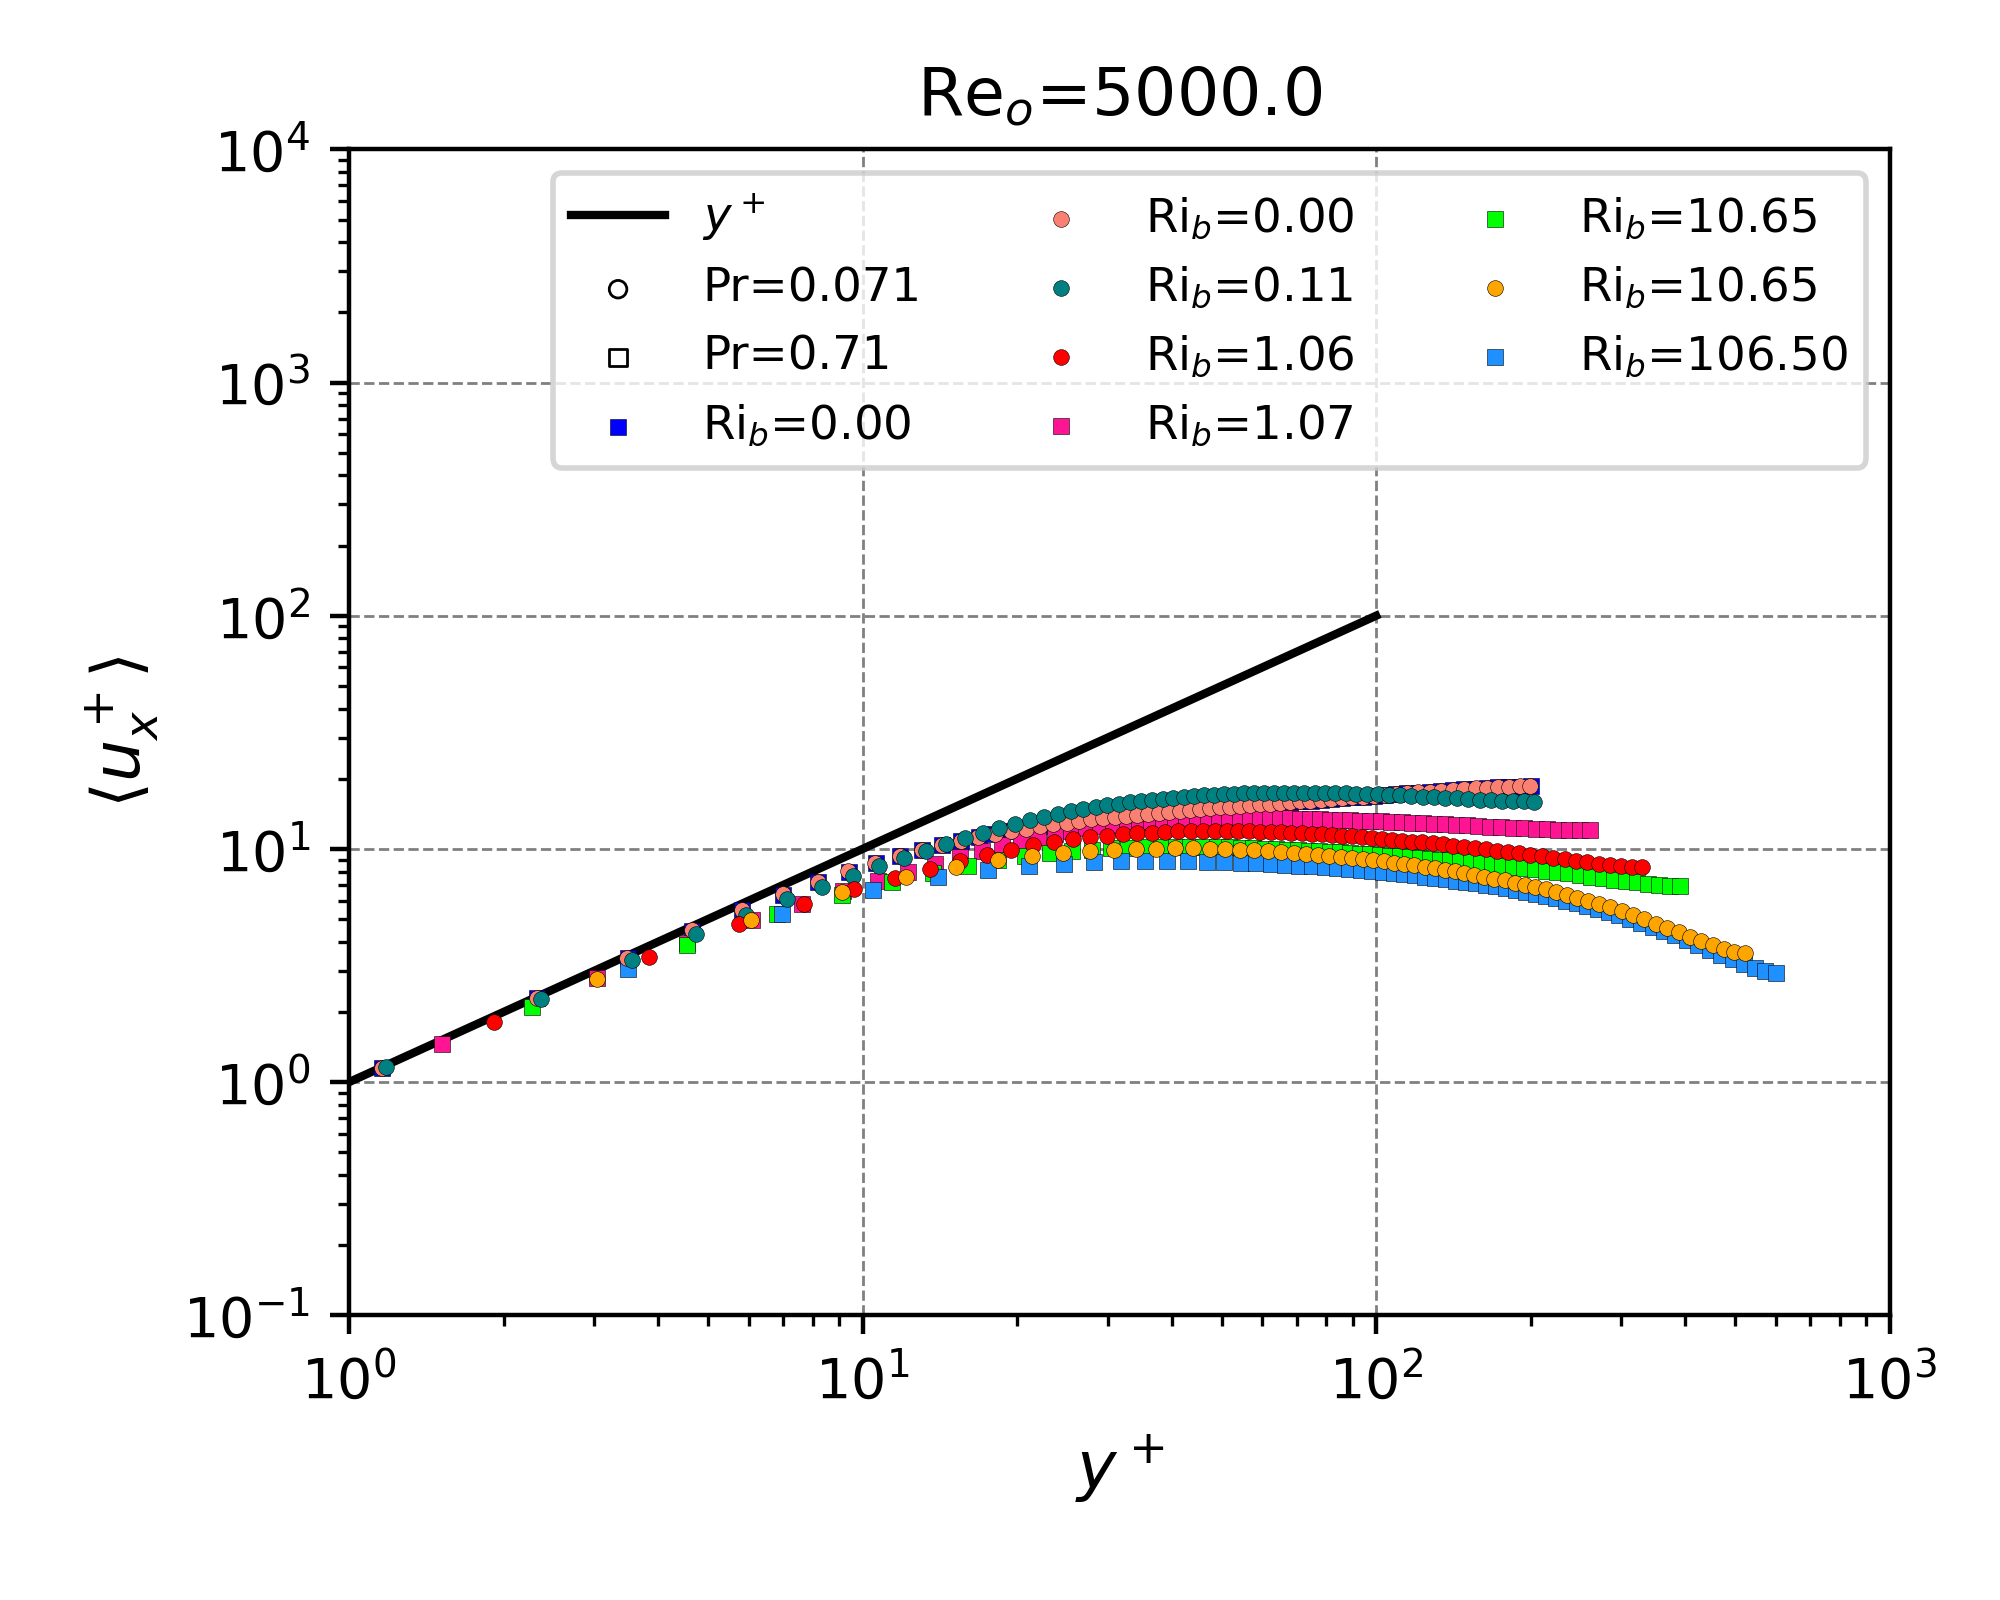
\includegraphics[width=0.5\textwidth]{figures/cap5/ux_mean_plus_log_profile.png}
  	  	\label{fig:plus-ux-Re5000-Prs}}
 	 \subfloat[]{
    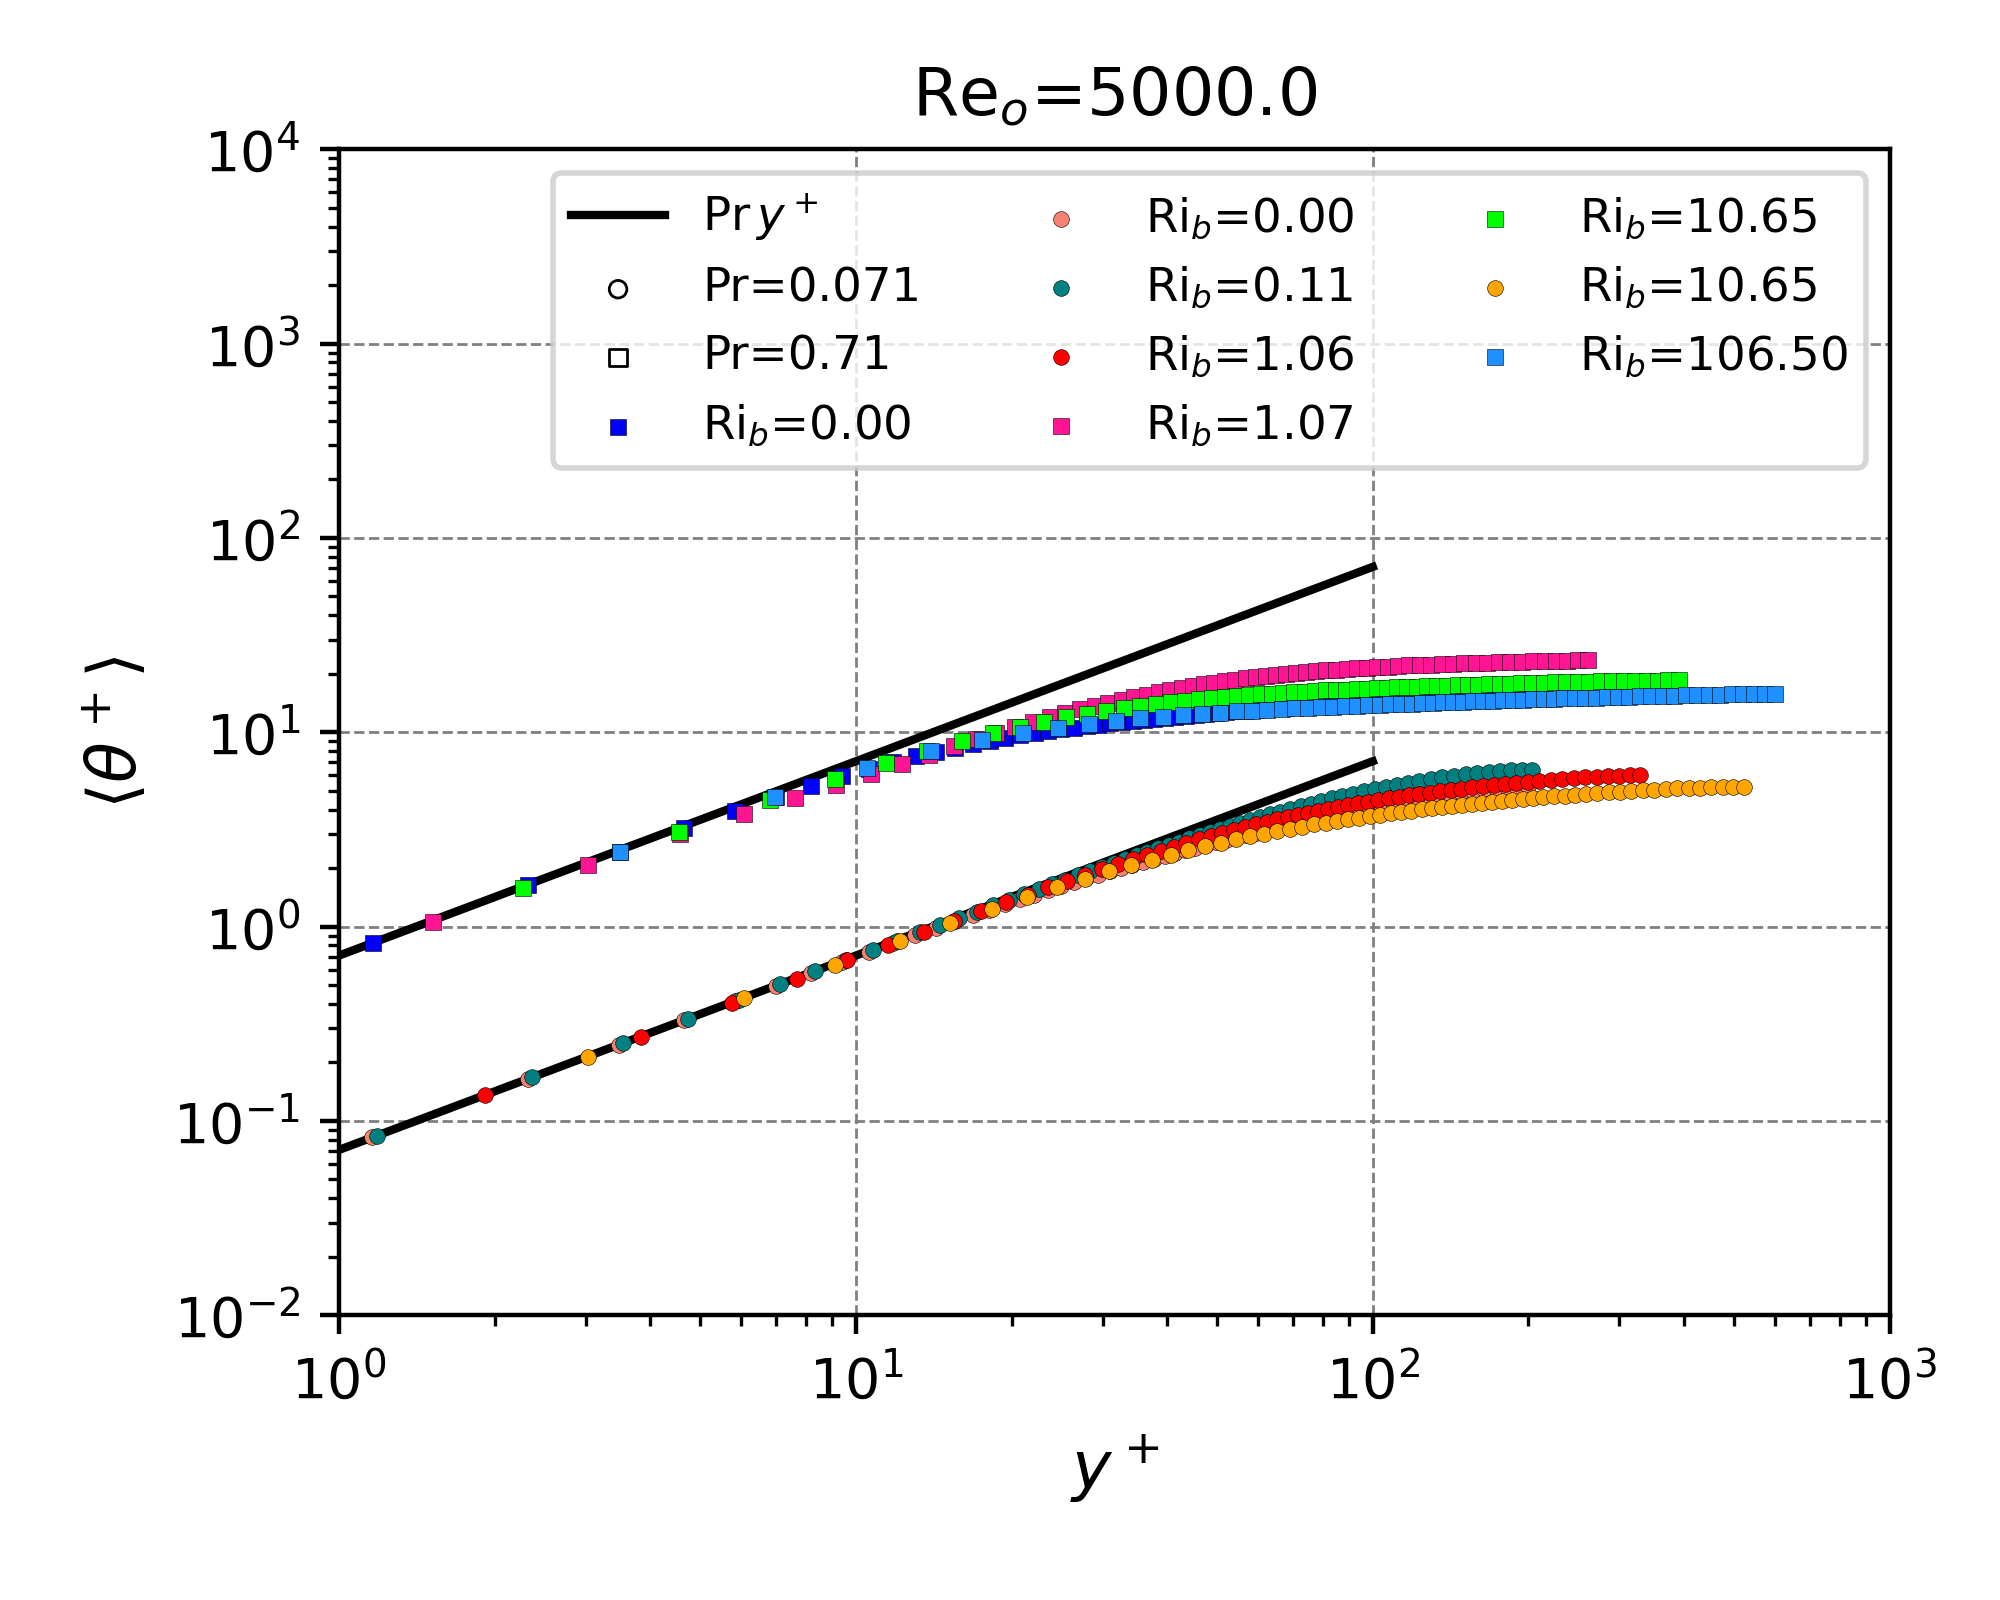
\includegraphics[width=0.5\textwidth]{figures/cap5/phi_mean_plus_log_profile.png}
    	\label{fig:plus-phi-Re5000-Prs}}
  \caption{Perfiles medios en unidades de pared para Re$_o$=5000 y Pr=0.071,0.71 y distintos valores de Ri$_b$.}
  \label{fig:Re5000-Pr071}
\end{figure}

%Por otra parte, en la Figura \ref{fig:plus-phi-Re5000-Prs} se presentan lo perfiles de temperatura media. Es posible aproximar la variación de la temperatura media cerca de la pared como proporcional a $y^+$ \cite{kawamura1998dns}:
%
%\begin{equation*}
%\langle \theta^* \rangle \simeq \text{Pr}\hspace{0.5mm} y^+
%\end{equation*}
% 
%Esta aproximación está representada en el gŕafico con lineas negras. Podemos ver que los casos con distinto Pr dicha aprox se corresponde con los datos de la simulación. Se aprecia que para el Pr más bajo la ley tiene un buen hasta $y^+ \sim 13$ mientras que para el más alto es menor, $y^+ \sim 7$. Esto está relacionado al hecho de que el fenómeno de conducción cerca la pared es más relevante que la convección para fluidos con difusividad térmica o Pr más bajos \cite{abregu2023dns}.



La Figura \ref{fig:plus-phi-Re5000-Prs} muestra los perfiles de temperatura adimensional media en unidades de pared. Cerca de la pared, la variación de la temperatura puede aproximarse por la relación lineal \cite{kawamura1998dns}
\begin{equation*}
\langle \theta^* \rangle \simeq \text{Pr}\hspace{0.5mm} y^+ ,
\end{equation*}
representada en la figura con líneas negras. Los resultados confirman esta ley para ambos números de Prandtl, aunque con distintos alcances: para el caso de Pr=0.071 la validez se extiende hasta $y^{+}\approx 30$, en concordancia con el trabajo de Zhou et al. \cite{zhou2024direct}. Sin embargo, para Pr=0.71 se reduce a $y^{+}\approx 7$. La diferencia se debe a que, en fluidos con menor difusividad térmica (Prandtl más bajo), el transporte de calor por conducción domina durante una mayor distancia normalizada desde la pared, retrasando la aparición del régimen convectivo predominante \cite{abregu2023dns}.






%\section{UHF vs UWT}
%
%En la sección [REF-VALIDACIONES] se utilizaron las simulaciones obtenidas por Guo y Prasser \cite{guo2022direct} para validar la herramienta numérica utilizada. El sistema estudiado por dichos autores corresponde a una configuración física distinta que al sistema estudiado en este trabajo, sin embargo, resulta útil comparar los perfiles de velocidad y temperatura, para entender en mayor profundidad el fenómeno de convección. En esta sección se pretende cotejar las dos configuraciones físicas establecidas: UHF\footnote{\textit{Uniform Heat Flux}} y UWT\footnote{\textit{Uniform Wall Temperature}}. El primero corresponde a los parámetros Re$_o$=3150, Pr=0.071 y Ri$_b$=0.67, y el segundo, a Re$_o$=3500, Pr=0.025 y Ri$_b$=0.5. Si bien los parámetros involucrados no son idénticos, están en el mismo orden de magnitud, para fines cualitativos, esto es más que adecuado para análizar la física detrás de ellos. Las Figuras \ref{fig:guocomp_ux} y \ref{fig:guocomp_phi} exponen los perfiles de velocidad en la dirección de la corriente y la temperatura de ambas configuraciones, respectivamente. En ambos casos se normaliza los perfiles con el máximo de la propia curva.  
%
%\begin{figure}[H]
%  \centering
%  \subfloat[]{
%    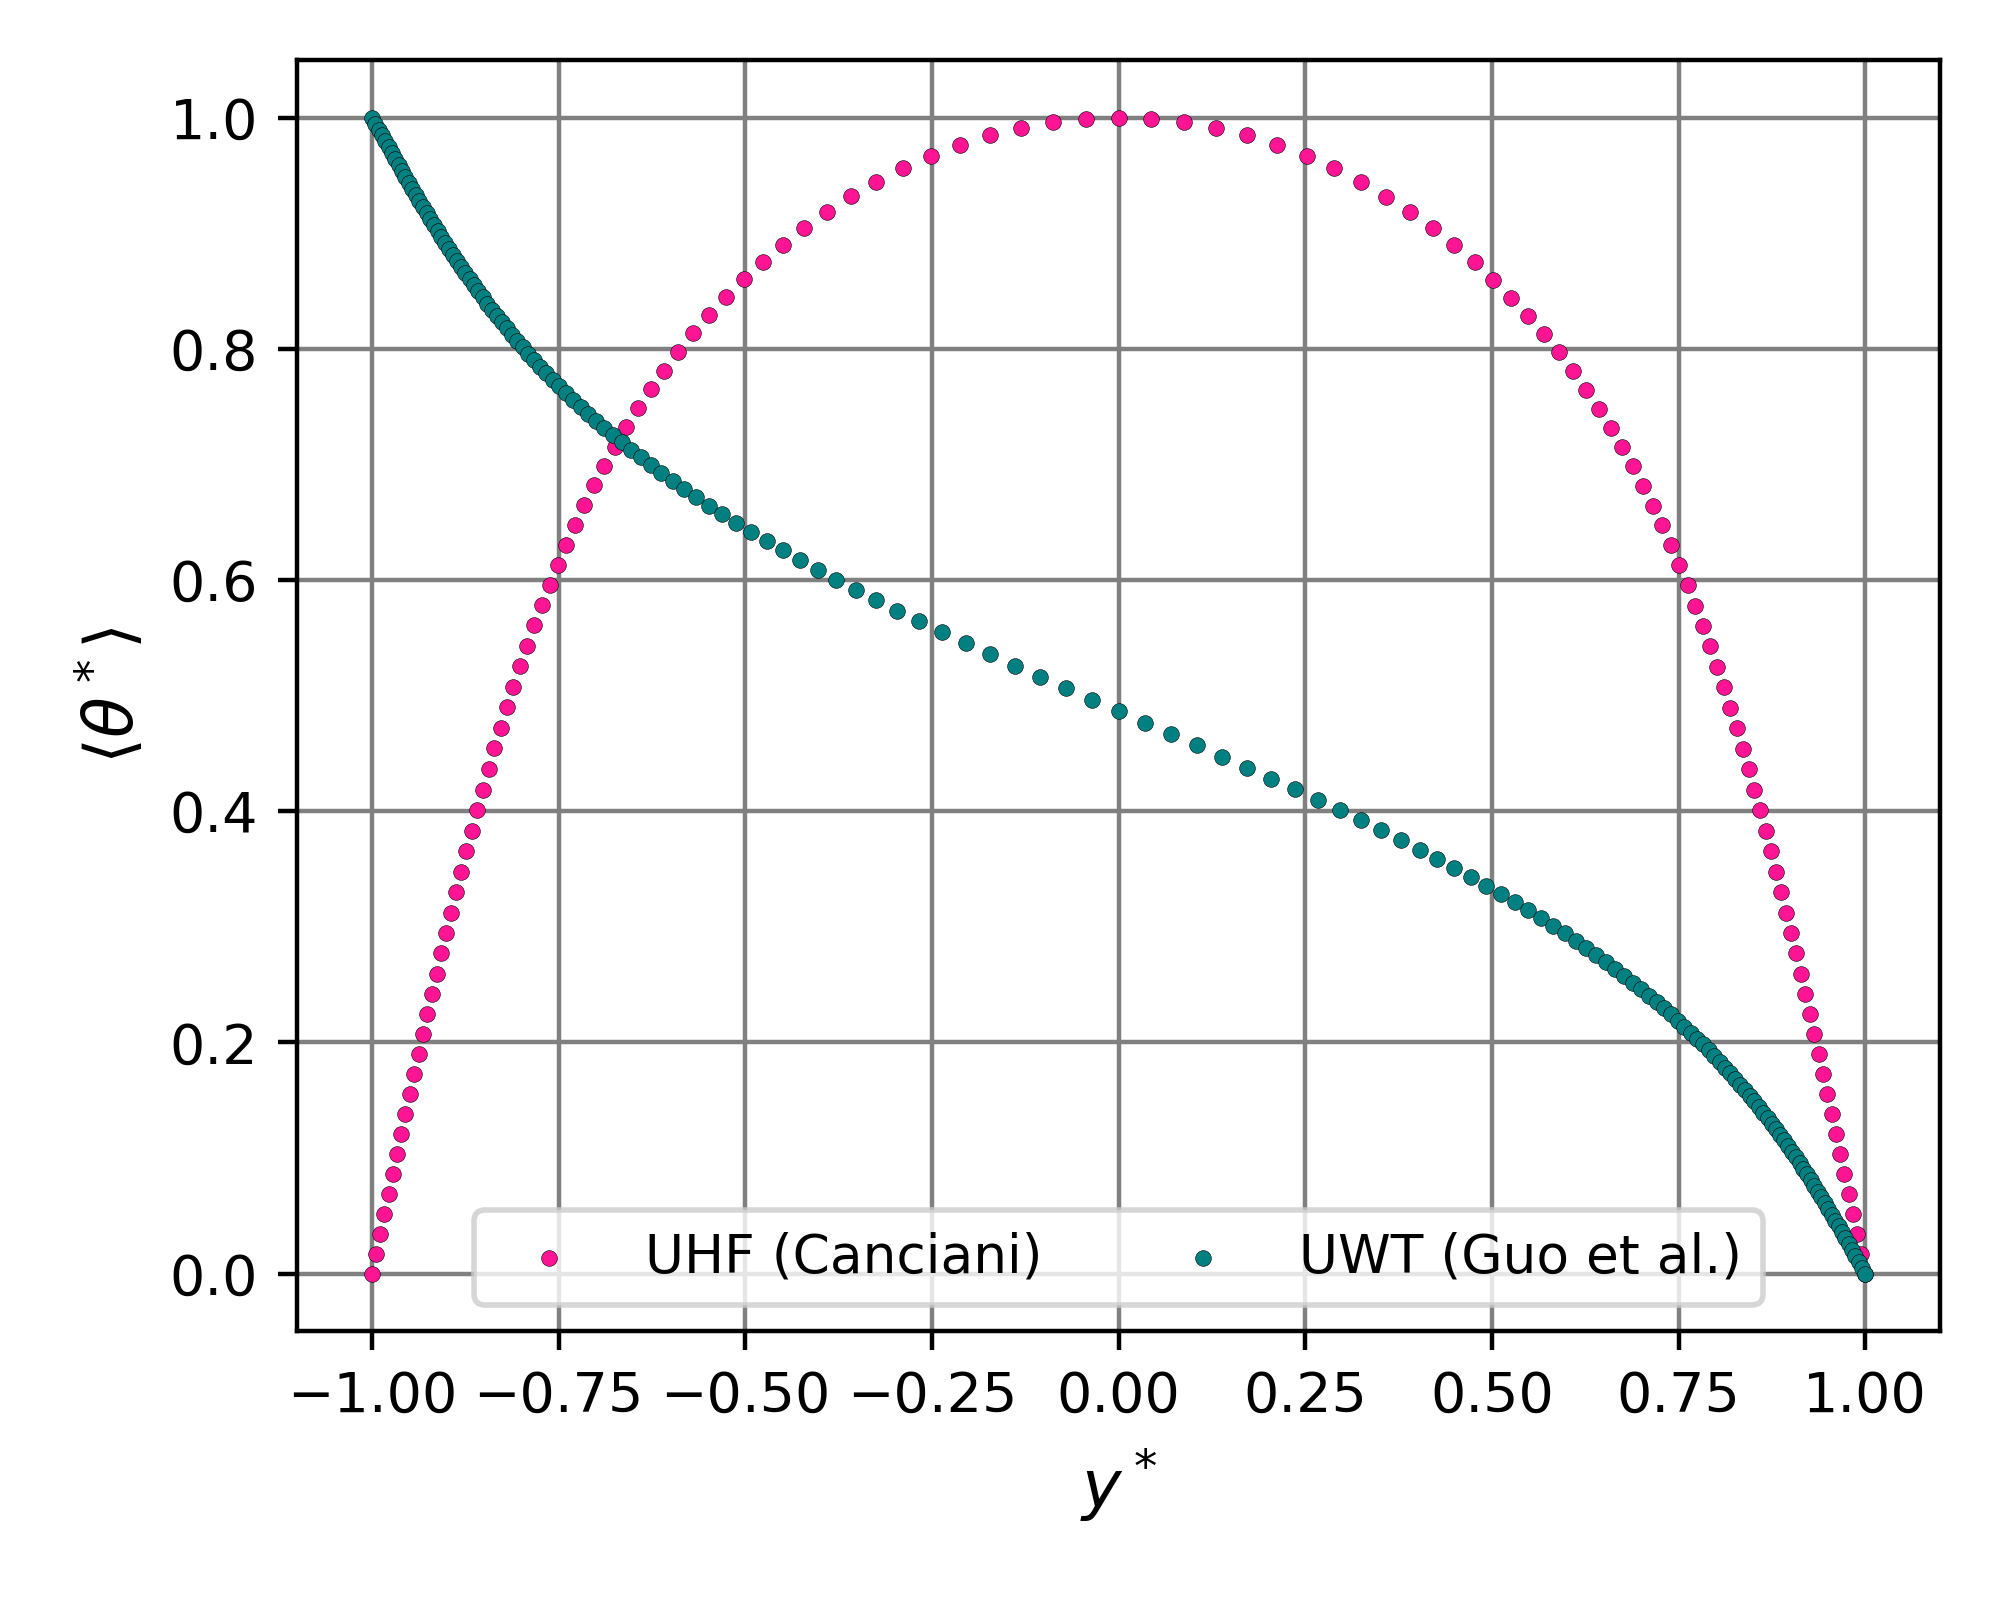
\includegraphics[width=0.49\textwidth]{figures/cap5/phi_mean_profile.png}
%    	\label{fig:guocomp_ux}}
%  \subfloat[]{
%    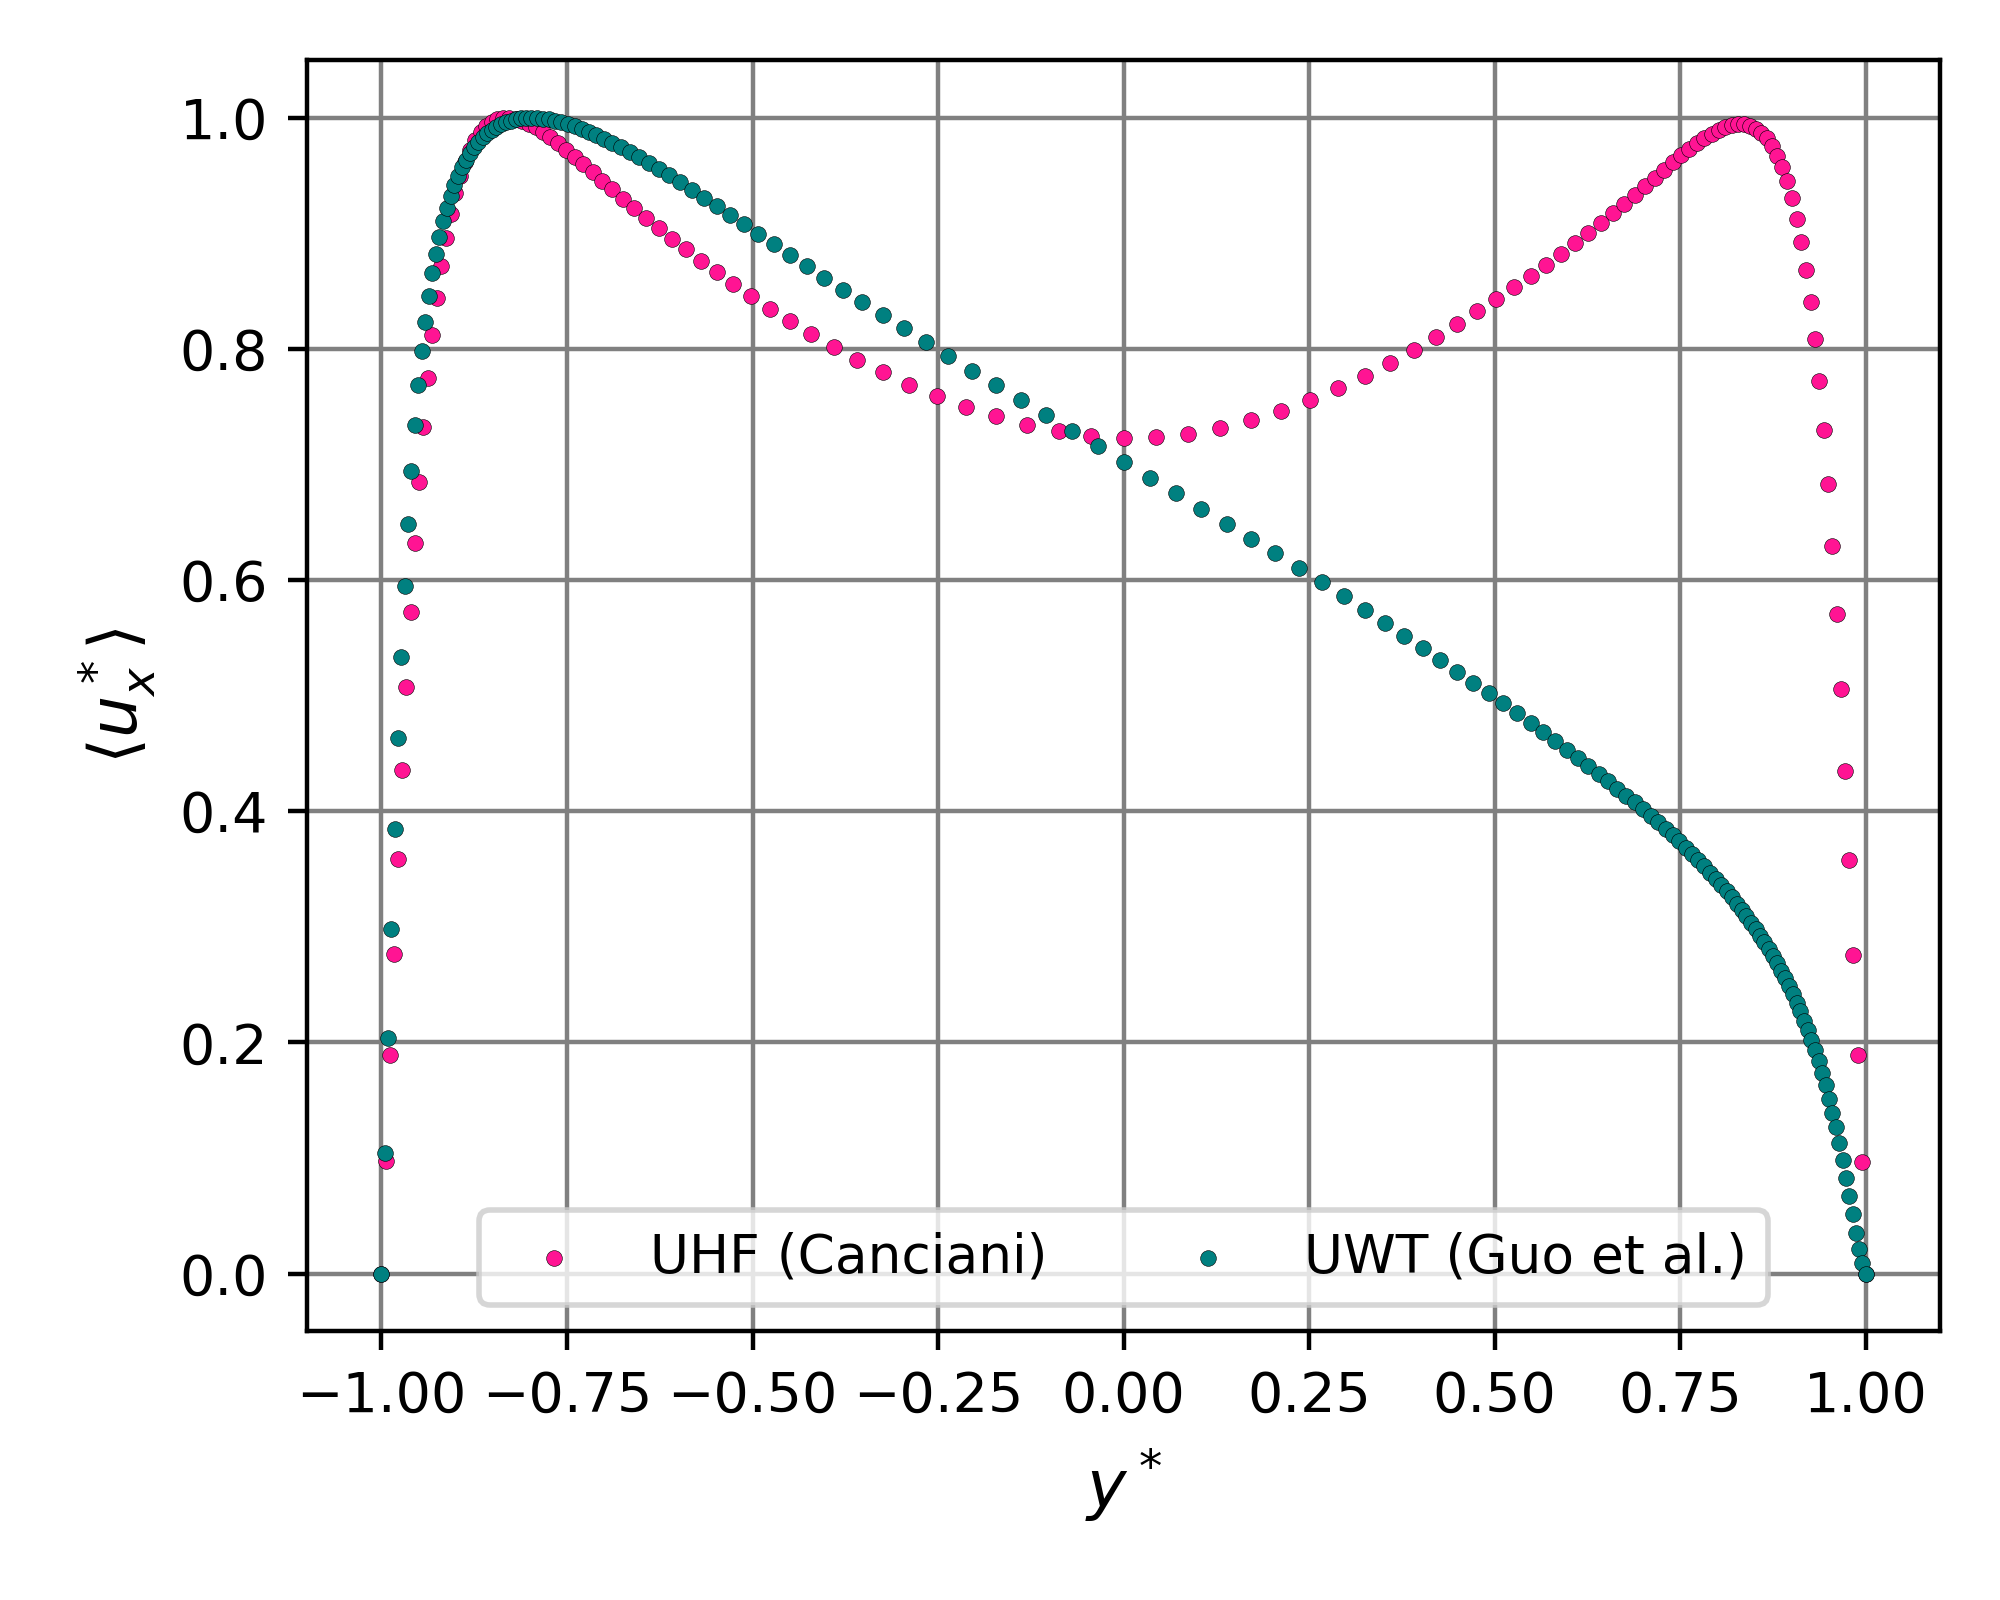
\includegraphics[width=0.49\textwidth]{figures/cap5/ux_mean_profile.png}
%    	\label{fig:guocomp_phi}}
%  \caption{Comparación entre los dos problemas.}
%  \label{fig:ux-guocomp}
%\end{figure}
%
%
%Una característica inmediata que se observa recae en la asimetría del los perfiles del caso UWT en comparación con UHF, lo que resulta claro debido a la asimetría del primero con respecto al segundo caso. 
%
%
%\textcolor{magenta}{seguir explicando la fisica de ambos casos.}



%\newpage
%\section{Número de Nusselt} \label{sec:nu}
%
%Desde una perspectiva ingenieríl, un parámetro importante que da información sobre la eficiencia de la transferencia de calor es el número de Nusselt (Nu), el cuál se define en la ecuación \ref{eq:nu}, donde $\overline{\theta_b}$ es la temperatura en \textit{bulk}.
%
%Un parámetro importante desde una perspectiva ingenieríl es el número de Nusselt (Nu), el cuál se define en la ecuación \ref{eq:nu}, donde $\overline{\theta_b}$ es la temperatura en \textit{bulk} (ecuación \ref{eq:tita_bulk}).
%
%\begin{equation}
%\text{Nu} = \frac{h L}{k} = \frac{2d \hspace*{1mm} q''_w}{k \hspace*{1mm} \overline{\theta^*_b}} = \frac{4}{3} \frac{Re_o Pr}{\overline{\theta^*_b}}	
%\label{eq:nu}
%\end{equation}
%
%\begin{equation*}
%\overline{\theta_b} = \frac{\frac{1}{A} \int \langle u_x \theta \rangle }{U_b} = \frac{\int^d_0 \langle u_x \theta \rangle \hspace*{0.5mm} dy }{\int^d_0 \langle u_x \rangle \hspace*{0.5mm} dy}
%\label{eq:tita_bulk}
%\end{equation*}
%
%En la Figura \ref{fig:nu_vs_bo} se presentan todos los valores de Nu obtenidos, graficados en función del número de boyancia Bo, definido en la ecuación \ref{eq:jackson_bo}, el cuál da una idea del \textit{ratio} entre las intensidad de las fuerzas boyantes y el la fuerza impulsora de la convección forzada. Los valores se contrastan con la correlación de Jackson et al. \cite{jackson1989studies}, expresada en la ecuación \ref{eq:jackson_corr}. Los valores Nu están normalizados con el Nu de convección forzada puro Nu$_{fc}$ el cuál es obtenido a partir de la correlación de Dittus-Boelter \cite{incropera}. Además, se añaden otros valores de Nu obtenidos mediante simulaciones DNS \cite{you2003direct} a modo de comparativa y se puede observar que los mismos se alinean con la tendencia de la correlación al igual que nuestro caso. 
%
%En la Figura \ref{fig:parity} se muestra un gráfico de paridad entre los números de Nusselt obtenidos por DNS, $Nu_{\text{DNS}}/Nu_{DB}$ (eje $x$), y los calculados con la correlación de Jackson, $Nu_{\text{corr}}/Nu_{DB}$ (eje $y$). La línea negra representa el acuerdo perfecto ($y=x$), mientras que las líneas azules punteadas señalan la banda de $\pm2\sigma$ alrededor de esa bisectriz. Puede verse que prácticamente todos los puntos experimentales se agrupan muy cerca de la bisectriz y permanecen dentro de la banda de $\pm2\sigma$, evidenciando que la correlación de Jackson reproduce con buena precisión los valores simulados a lo largo de todo el rango de $Nu_{\text{DNS}}/Nu_{DB}$ considerado.
%
%
%Pueden distinguir 3 regiones principales
%\begin{itemize}
% \item[$\bullet$] para Bo $\lesssim$ $10^{-6}$ el valor Nu es practicamente igual a Nu$_{fc}$, es decir, domina la convección forzada,
% \item[$\bullet$] en el rango $10^{-6}$ $\lesssim$ Bo $\lesssim$ $3 \times 10^{-5}$ se observa una caida y una recuperación del número de Nusselt, revelando la existencia de una región donde la transferencia de calor empeora por debajo del caso únicamente forzada y que luego retoma su condición original,
% \item[$\bullet$] por último, para Bo $\gtrsim$ $3 \times 10^{-5}$ la transferencia de calor aumenta notoriamente, impulsado por las corrientes de convección natural que en esta región tiene mayor preponderancia.
%\end{itemize}
%
%%\vspace*{-1.5cm}
%
%\begin{equation}
%\text{Bo}= \frac{Gr*}{{\text{Re}_D}^{3.425} \hspace*{1mm} \text{Pr}^{0.8} }
%\label{eq:jackson_bo}
%\end{equation}
%
%\begin{equation}
%\frac{\text{Nu}}{\text{Nu}_{fc}}= \left\vert  1 - 8 \times 10^4 \hspace*{0.5mm} \text{Bo} \hspace*{0.5mm} \left( \frac{\text{Nu}}{\text{Nu}_{fc}} \right)^{-2}  \right\vert^{0.46}
%\label{eq:jackson_corr} 
%\end{equation}
%
%
%\begin{figure}[H]
%  \centering
%  \subfloat[]{
%    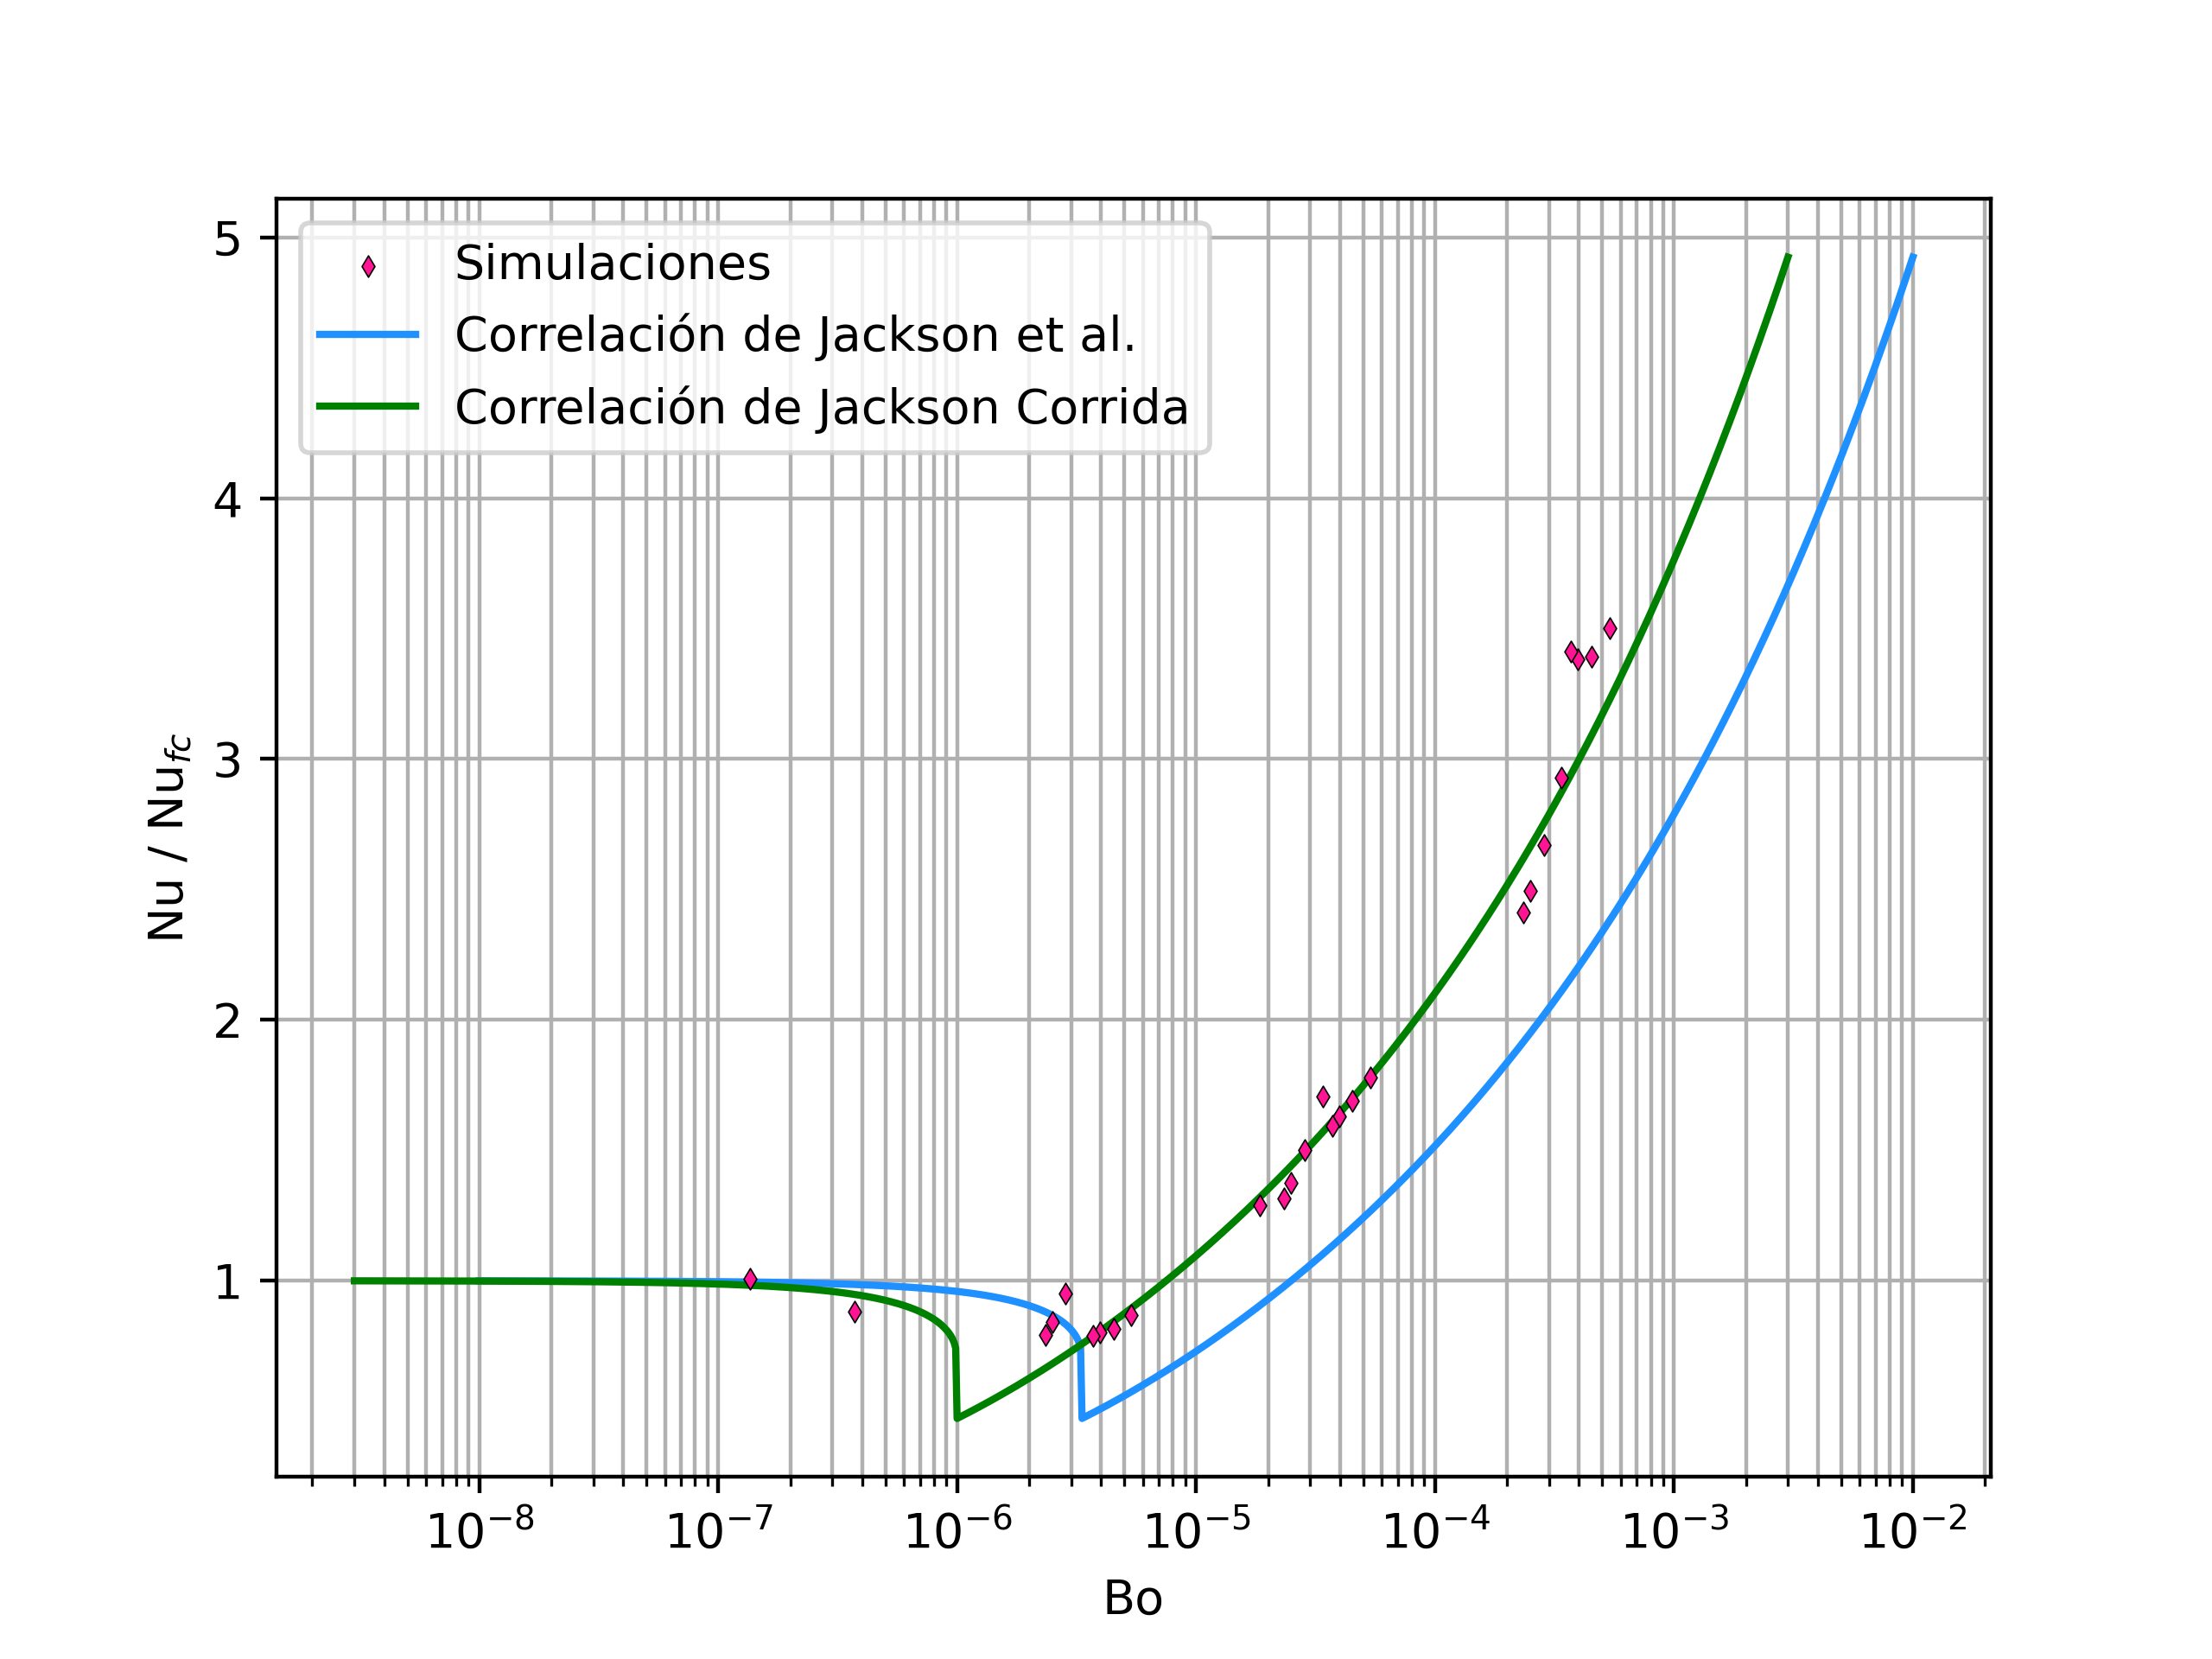
\includegraphics[width=0.49\textwidth]{figures/cap5/nusselt_corr/Nu_vs_Bo_Jackson.png}
%    	\label{fig:nu_vs_bo}}
%  \subfloat[]{
%    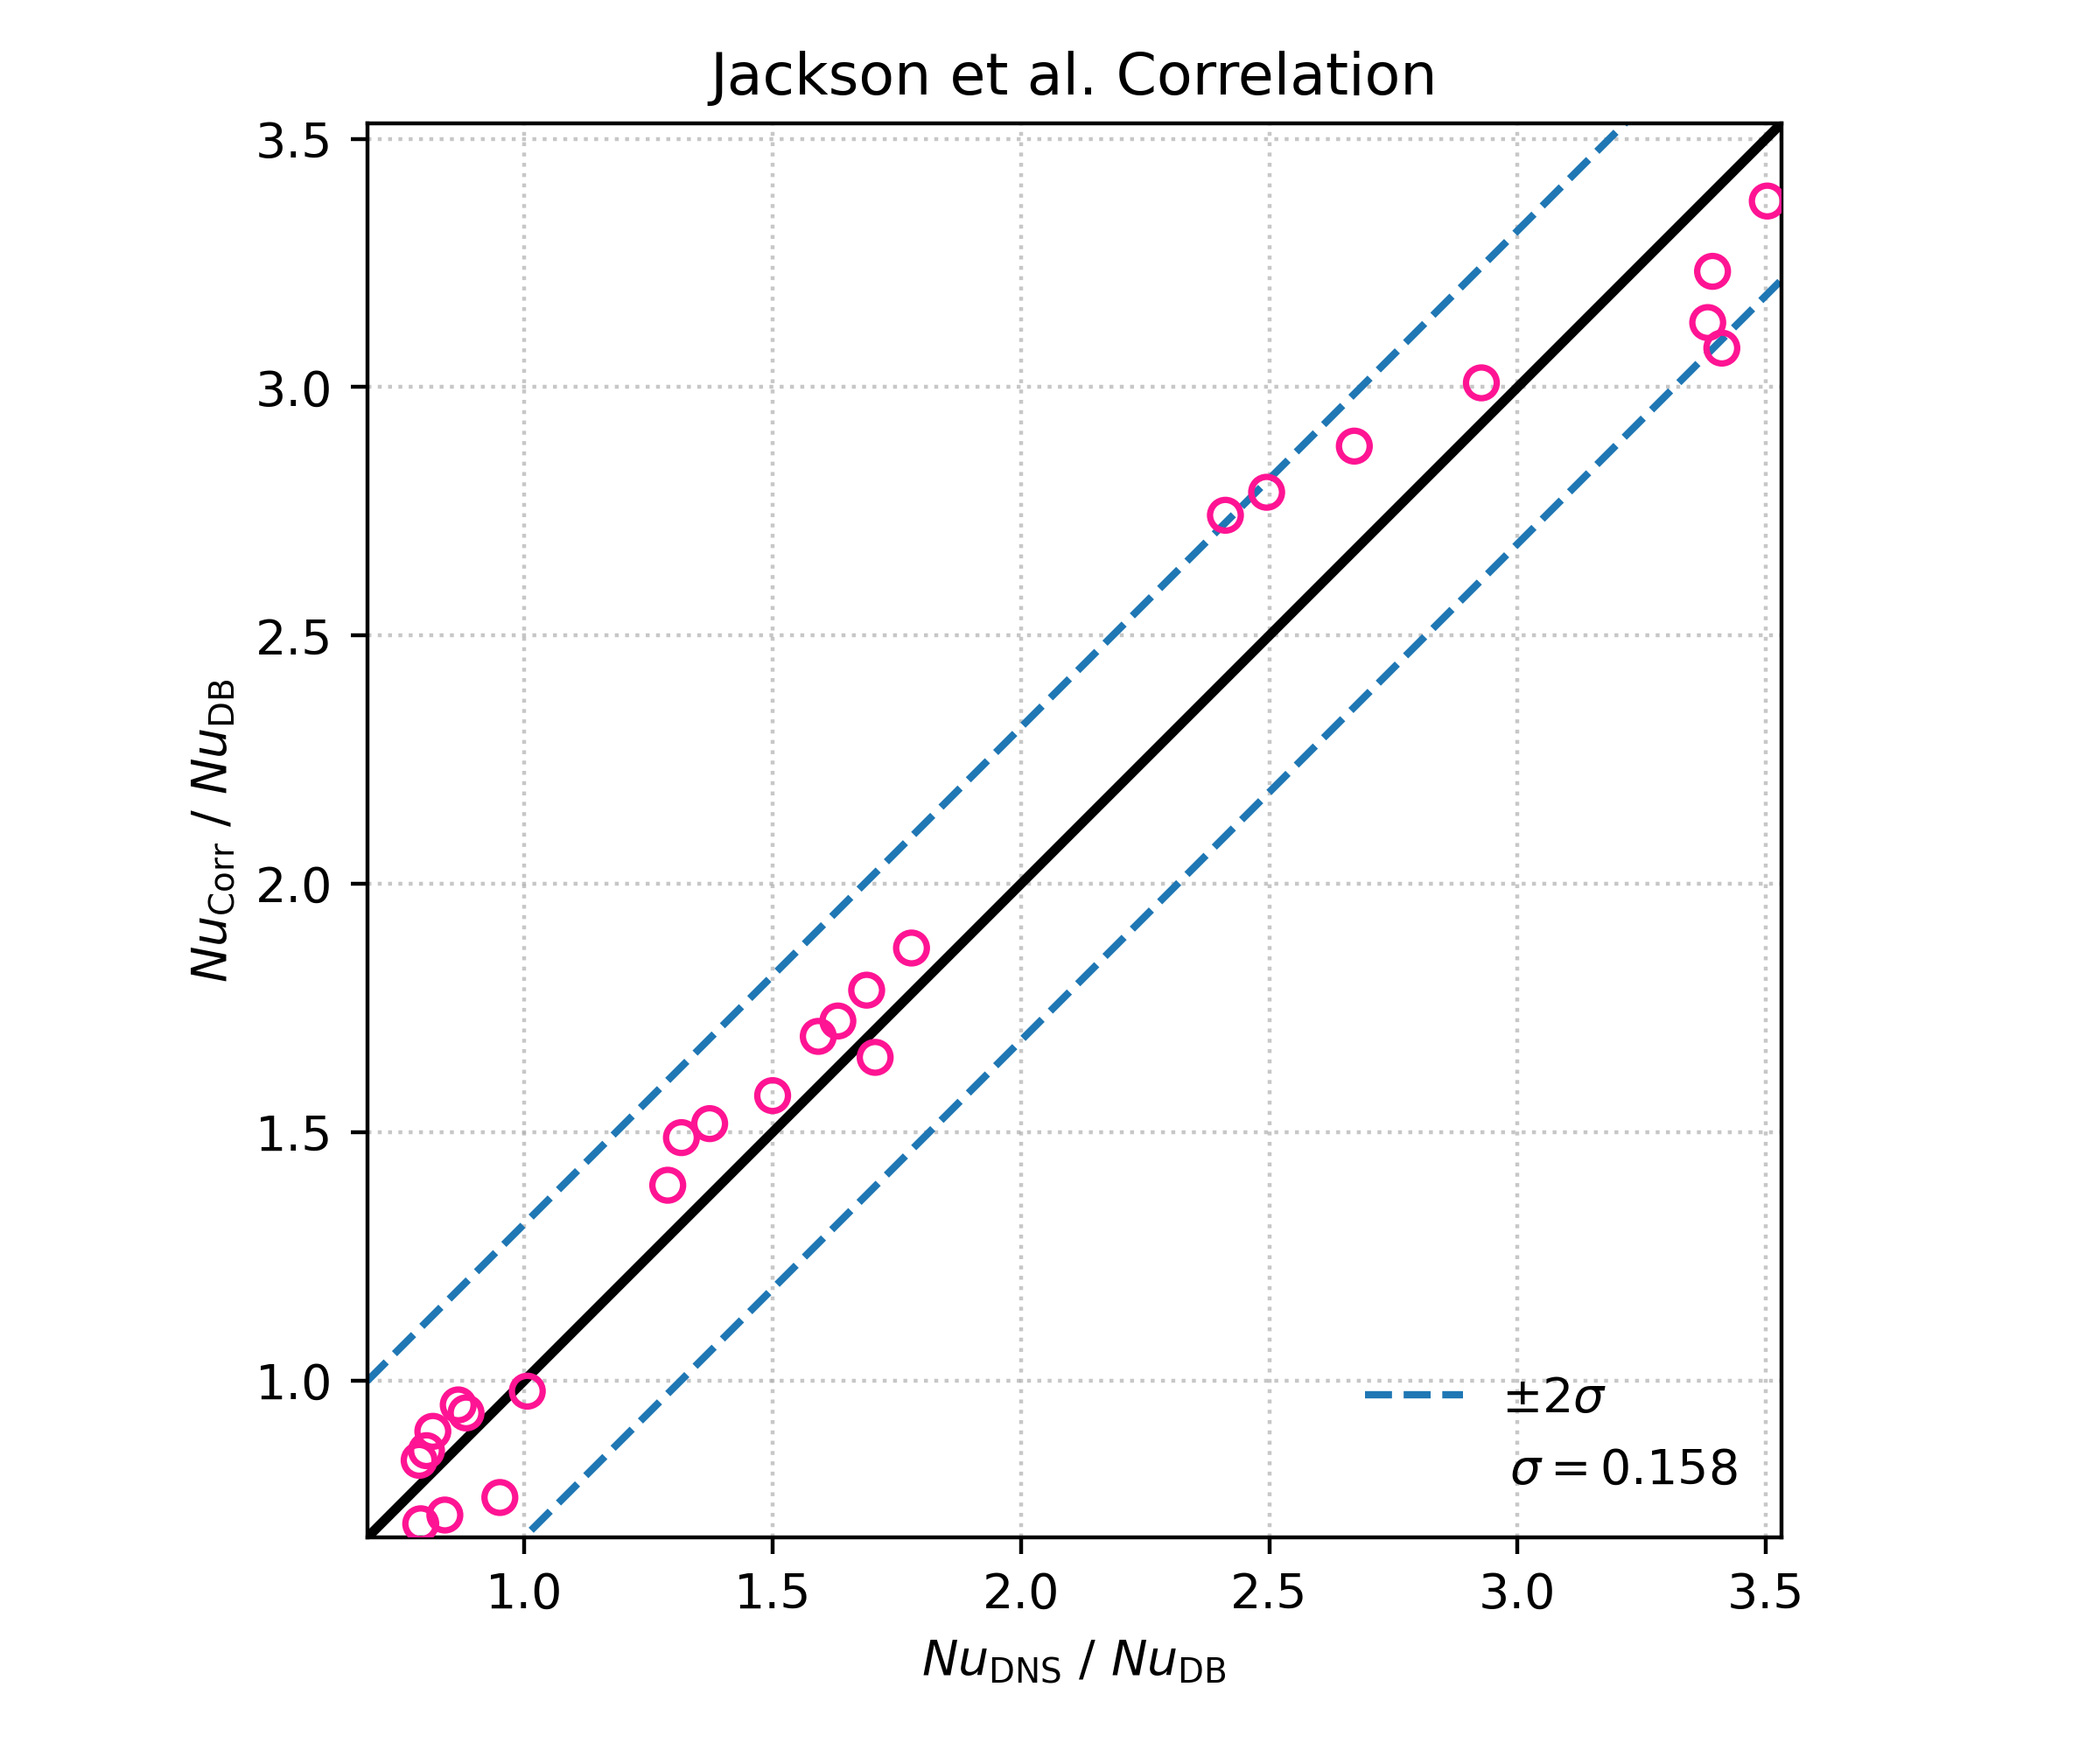
\includegraphics[width=0.49\textwidth]{figures/cap5/nusselt_corr/jackson_parity.png}
%    	\label{fig:parity}}
%    
%  \caption{Aquí $Bo = Gr / (Re^{3,425} Pr^{0,8})$}
%  \label{fig:nusselt}
%\end{figure}
%
%La caída del número de Nu con el aumento de la fuerza boyante puede interpretarse en términos del perfil de velocidad en la dirección de la corriente. En la sección \ref{sec:velo_temp} se comentó que cuando la convección natural y la convección forzada actúan en la misma dirección el fluido es acelerado en las zonas cercanas a las paredes y, en virtud de la conservación de masa, el flujo se desacelera en la región central. En virtud de esta premisa es posible acercarse a un entendimiento cualitativo. De acuerdo al modelo de Prandtl \cite{Prandtl1942}, la transferencia de calor ocurre mediante 2 mecanísmo principales: transferencia por conducción en la subcapa viscosa y por el flujo de calor turbulento en la dirección normal a la pared, esto es, $q''_y \aprox \rho \hspace{0.5mm} c_P \hspace{0.5mm} \langle u^{*'}_y \theta^{*'} \rangle$. De acuerdo a Aicher y Martin \cite{aicher1997}, en la zona cercana al borde de la capa viscosa, el flujo $q''_y$ es proporcional a la producción de turbulencia el cuál es la suma de la \textit{Shear-Production} y \textit{Buoyancy-Production}, cantidades (o \textit{budgets}) provenientes del balance de la cinética turbulenta $k$ (Apéndice \ref{apen:budgets}). En este sentido, la producción de turbulencia dependerá de la diferencia de velocidades entre el centro del canal y la zona próxima a la pared.
%
%Así, dado que la boyancia produce un aumento de la velocidad cerca de las paredes, es posible apreciar una rango de Ri$b$ ($10^{-6}$ $\lesssim$ Bo $\lesssim$ $3 \times 10^{-5}$ de la Figura \ref{fig:nu_vs_bo}) para los cuales ésta diferencia es, o bien cero, o bien muy pequeña. A medida que la fuerza boyante sigue incrementando, dicha diferencia de velocidades (o gradiente) crece, y en consecuencia, aumenta la producción de turbulencia, el flujo de calor turbulento normal y transferencia de calor que se refeja en un aumento del Nu.  
%
%
%
%


%\begin{figure}[H]
%  \centering
%   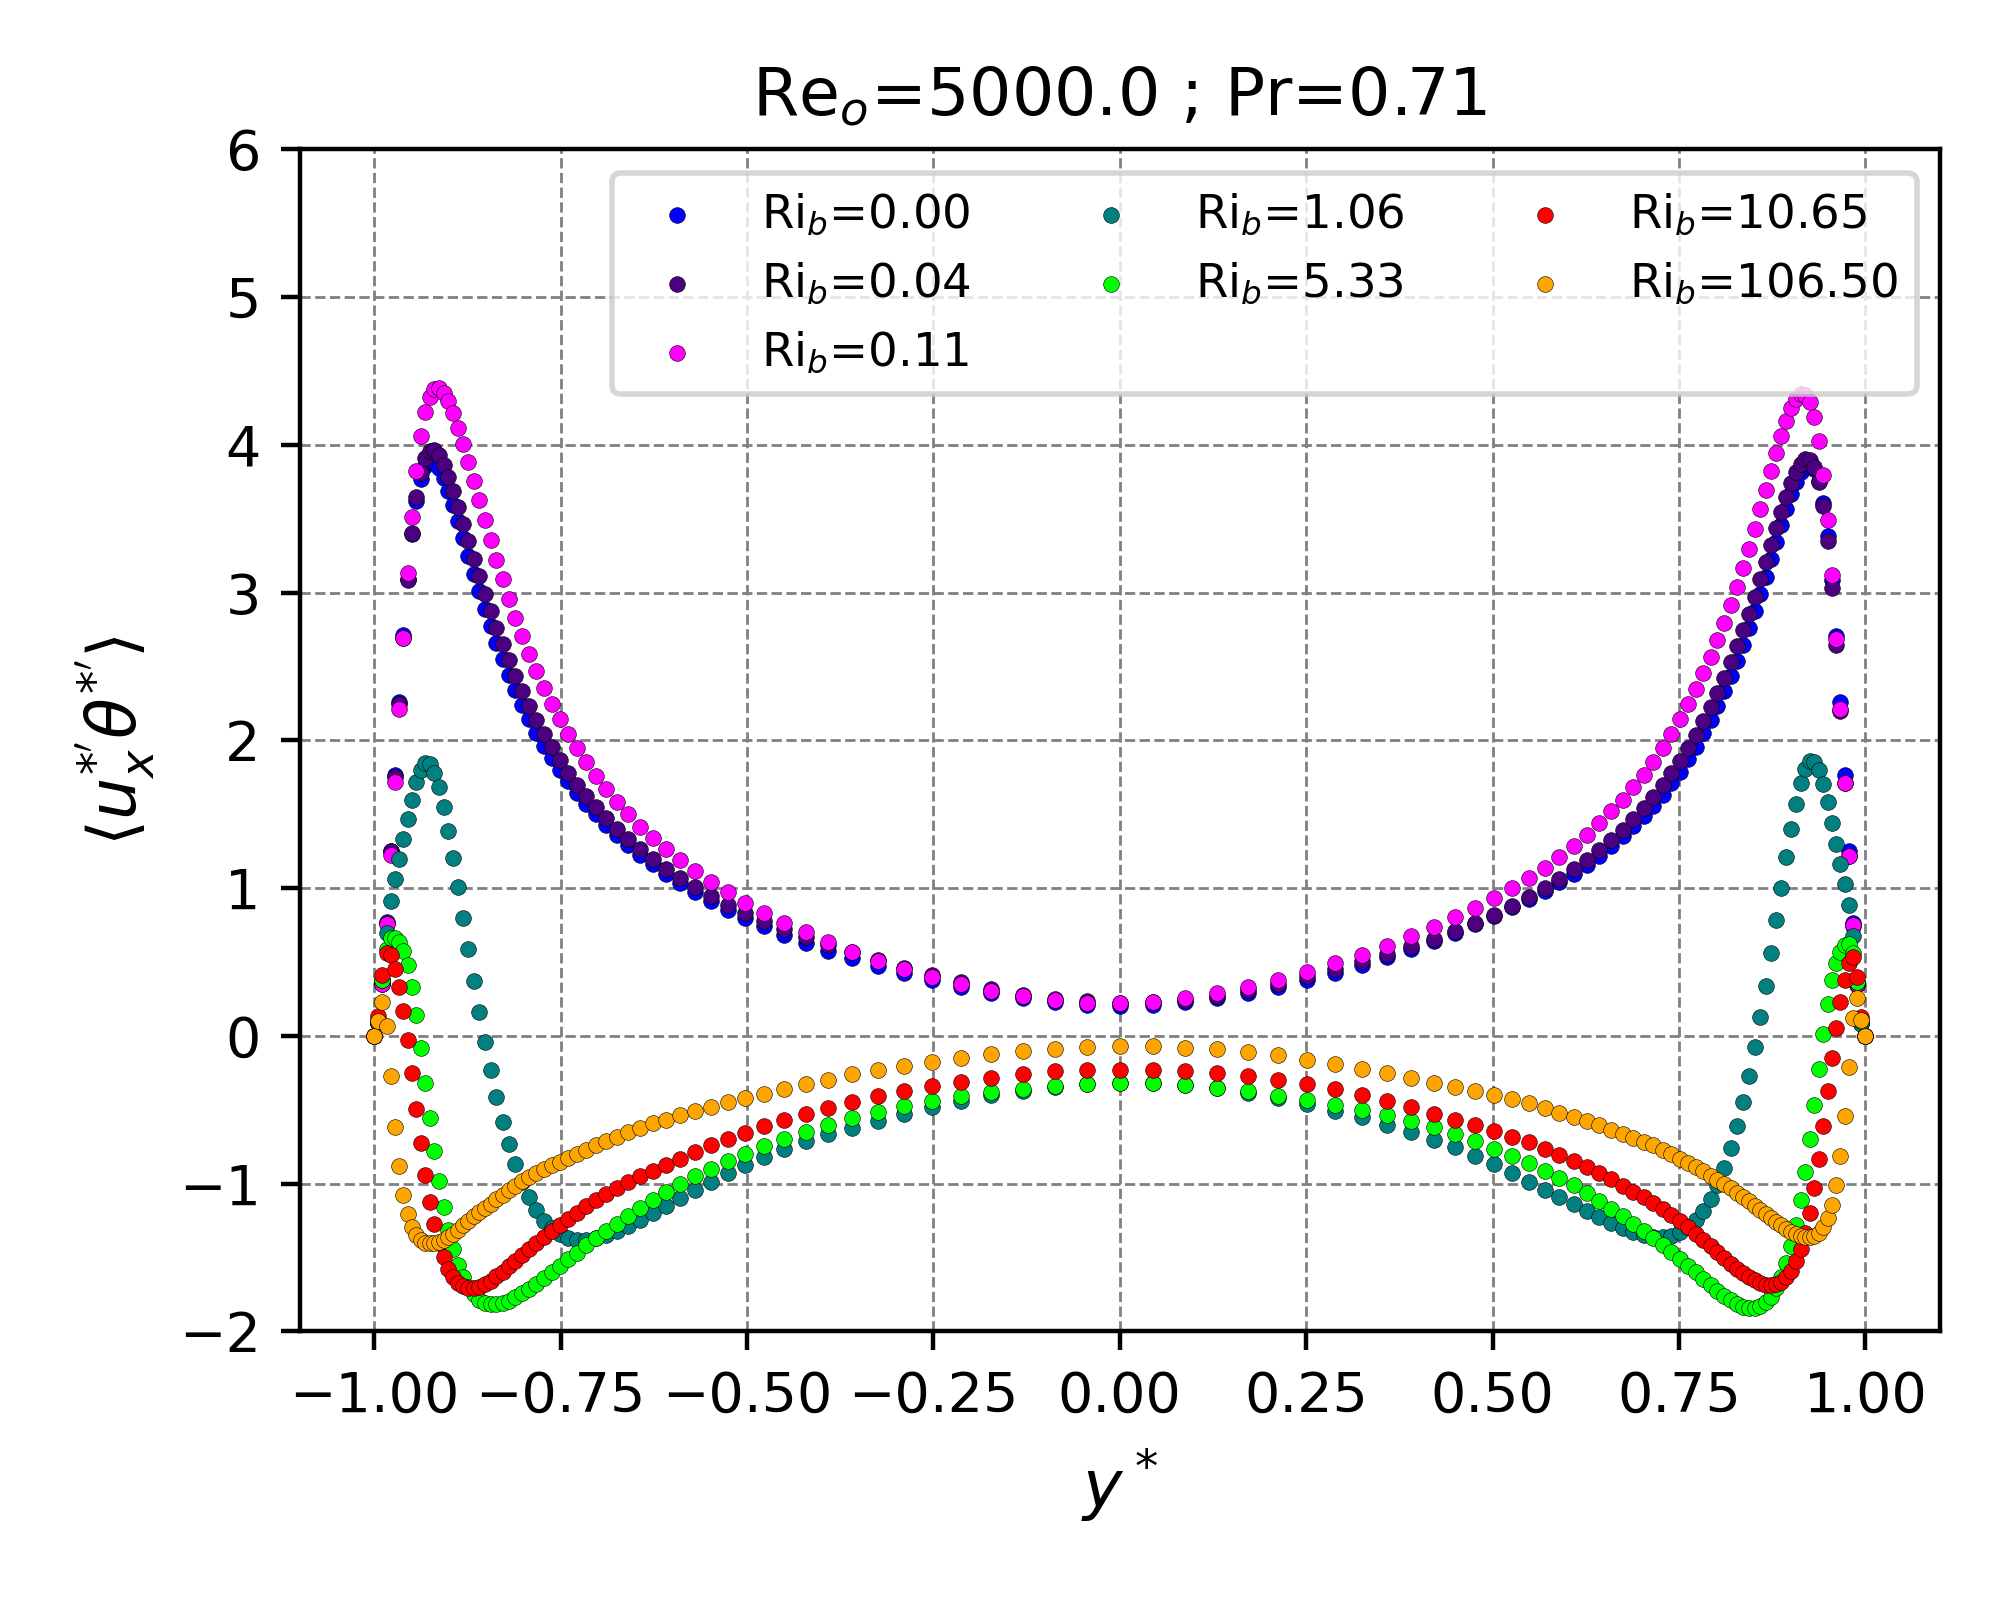
\includegraphics[width=0.6\textwidth]{figures/cap5/Re5000-Pr071/uphif_profile.png}
%   	\label{fig:uphif-Re5000-Pr071}
%  \caption{\textcolor{red}{Acá va el flujo de calor turbulento normal a la pared ... solo que todavía no pude hacerlo porque el cluster está inactivo ...}}
%\end{figure}



\newpage
\section{Número de Nusselt} \label{sec:nu}

Desde una perspectiva ingenieril, el número de Nusselt (Nu) es un indicador clave de la eficiencia de la transferencia de calor. Su definición se presenta en la ecuación \ref{eq:nu}, donde $\langle \theta_b \rangle$ es la temperatura \textit{bulk} (ecuación \ref{eq:tita_bulk}).

\begin{equation}
\text{Nu} = \frac{h L}{k} = \frac{2d}{k} \frac{q''_w}{\langle \theta_b \rangle} = \frac{4}{3} \frac{Re_o Pr}{\langle \theta^*_b \rangle}	
\label{eq:nu}
\end{equation}

\begin{equation}
\langle \theta_b \rangle = \frac{\int_{-d}^{+d} \langle u_x \theta \rangle \, dy}{\int_{-d}^{+d} \langle u_x \rangle \, dy} = \frac{\int_{-d}^{+d} \langle u_x \theta \rangle }{2d \, U_b}
\label{eq:tita_bulk}
\end{equation}

La Figura \ref{fig:nu_vs_bo} muestra los valores de Nu obtenidos en función del número de boyancia Bo (ecuación \ref{eq:jackson_bo}), que cuantifica la relación entre las fuerzas boyantes y la fuerza impulsora de la convección forzada. Estos resultados se comparan con la correlación de Jackson et al. \cite{jackson1989studies} (ecuación \ref{eq:jackson_corr}). Los valores de Nu se normalizan con el valor correspondiente a convección forzada pura, Nu$_{fc}$, evaluado mediante la correlación de Dittus-Boelter \cite{incropera}. También se añaden datos provenientes de simulaciones DNS \cite{you2003direct} que se alinean con la misma tendencia.

En la Figura \ref{fig:parity} se presenta un gráfico de paridad entre $Nu_{\text{DNS}}/Nu_{DB}$ (eje $x$) y $Nu_{\text{corr}}/Nu_{DB}$ (eje $y$). La línea negra indica el acuerdo perfecto ($y=x$) y las líneas azules punteadas delimitan la banda de $\pm2\sigma$ (con $\sigma$=0.158). La concentración de puntos dentro de esta banda confirma que la correlación de Jackson reproduce con buena precisión los valores simulados.

A partir de la Figura \ref{fig:nu_vs_bo} se distinguen tres regiones:

\begin{itemize}
  \item[$\bullet$] Bo $\lesssim 10^{-6}$: Nu se mantiene prácticamente igual a Nu$_{fc}$; domina la convección forzada.
  \item[$\bullet$] $10^{-6} \lesssim$ Bo $\lesssim 3 \times 10^{-5}$: Nu desciende y luego se recupera, indicando una zona donde la transferencia de calor empeora temporalmente respecto al caso puramente forzado.
  \item[$\bullet$] Bo $\gtrsim 3 \times 10^{-5}$: Nu crece de forma marcada, impulsado por la mayor relevancia de la convección natural.
\end{itemize}

\begin{equation}
\text{Bo}= \frac{Gr*}{\text{Re}_D^{3.425} \hspace*{1mm} \text{Pr}^{0.8}}
\label{eq:jackson_bo}
\end{equation}

\begin{equation}
\frac{\text{Nu}}{\text{Nu}_{fc}} =
\left\vert 1 - 8 \times 10^4 \hspace*{0.5mm} \text{Bo}
\left( \frac{\text{Nu}}{\text{Nu}_{fc}} \right)^{-2} \right\vert^{0.46}
\label{eq:jackson_corr}
\end{equation}

\begin{figure}[H]
  \centering
  \subfloat[]{
    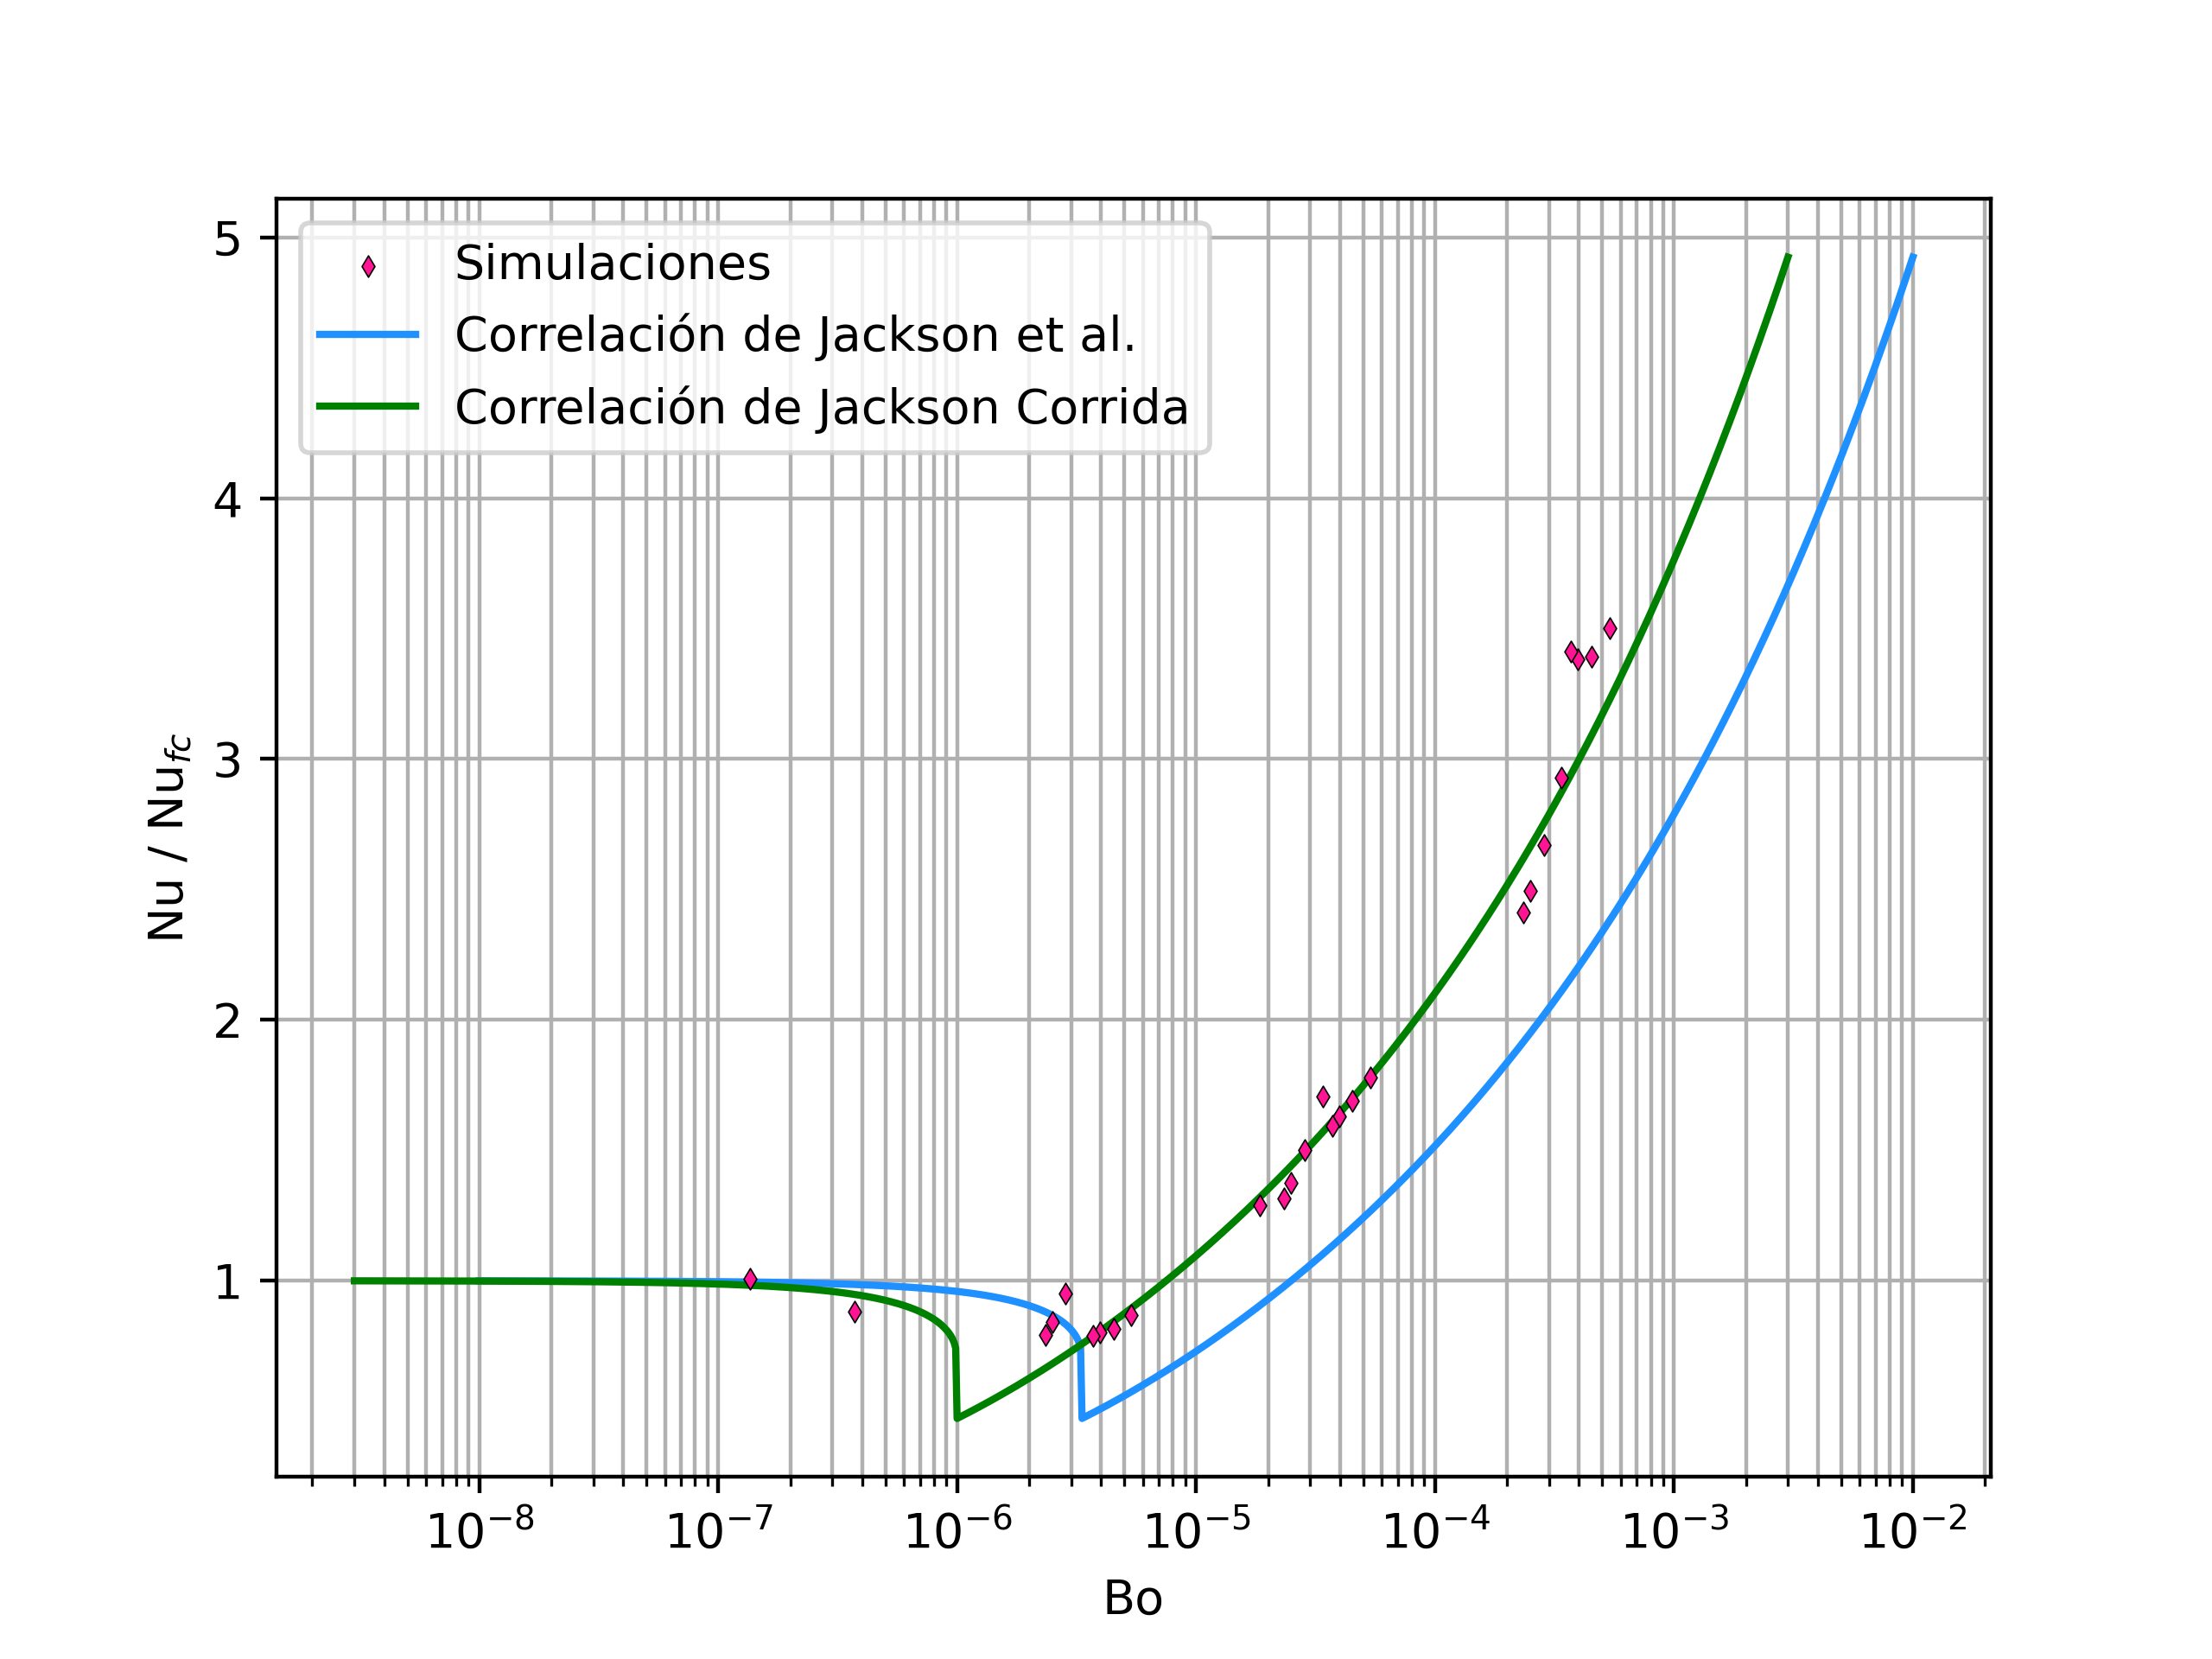
\includegraphics[width=0.49\textwidth]{figures/cap5/nusselt_corr/Nu_vs_Bo_Jackson.png}
    \label{fig:nu_vs_bo}}
  \subfloat[]{
    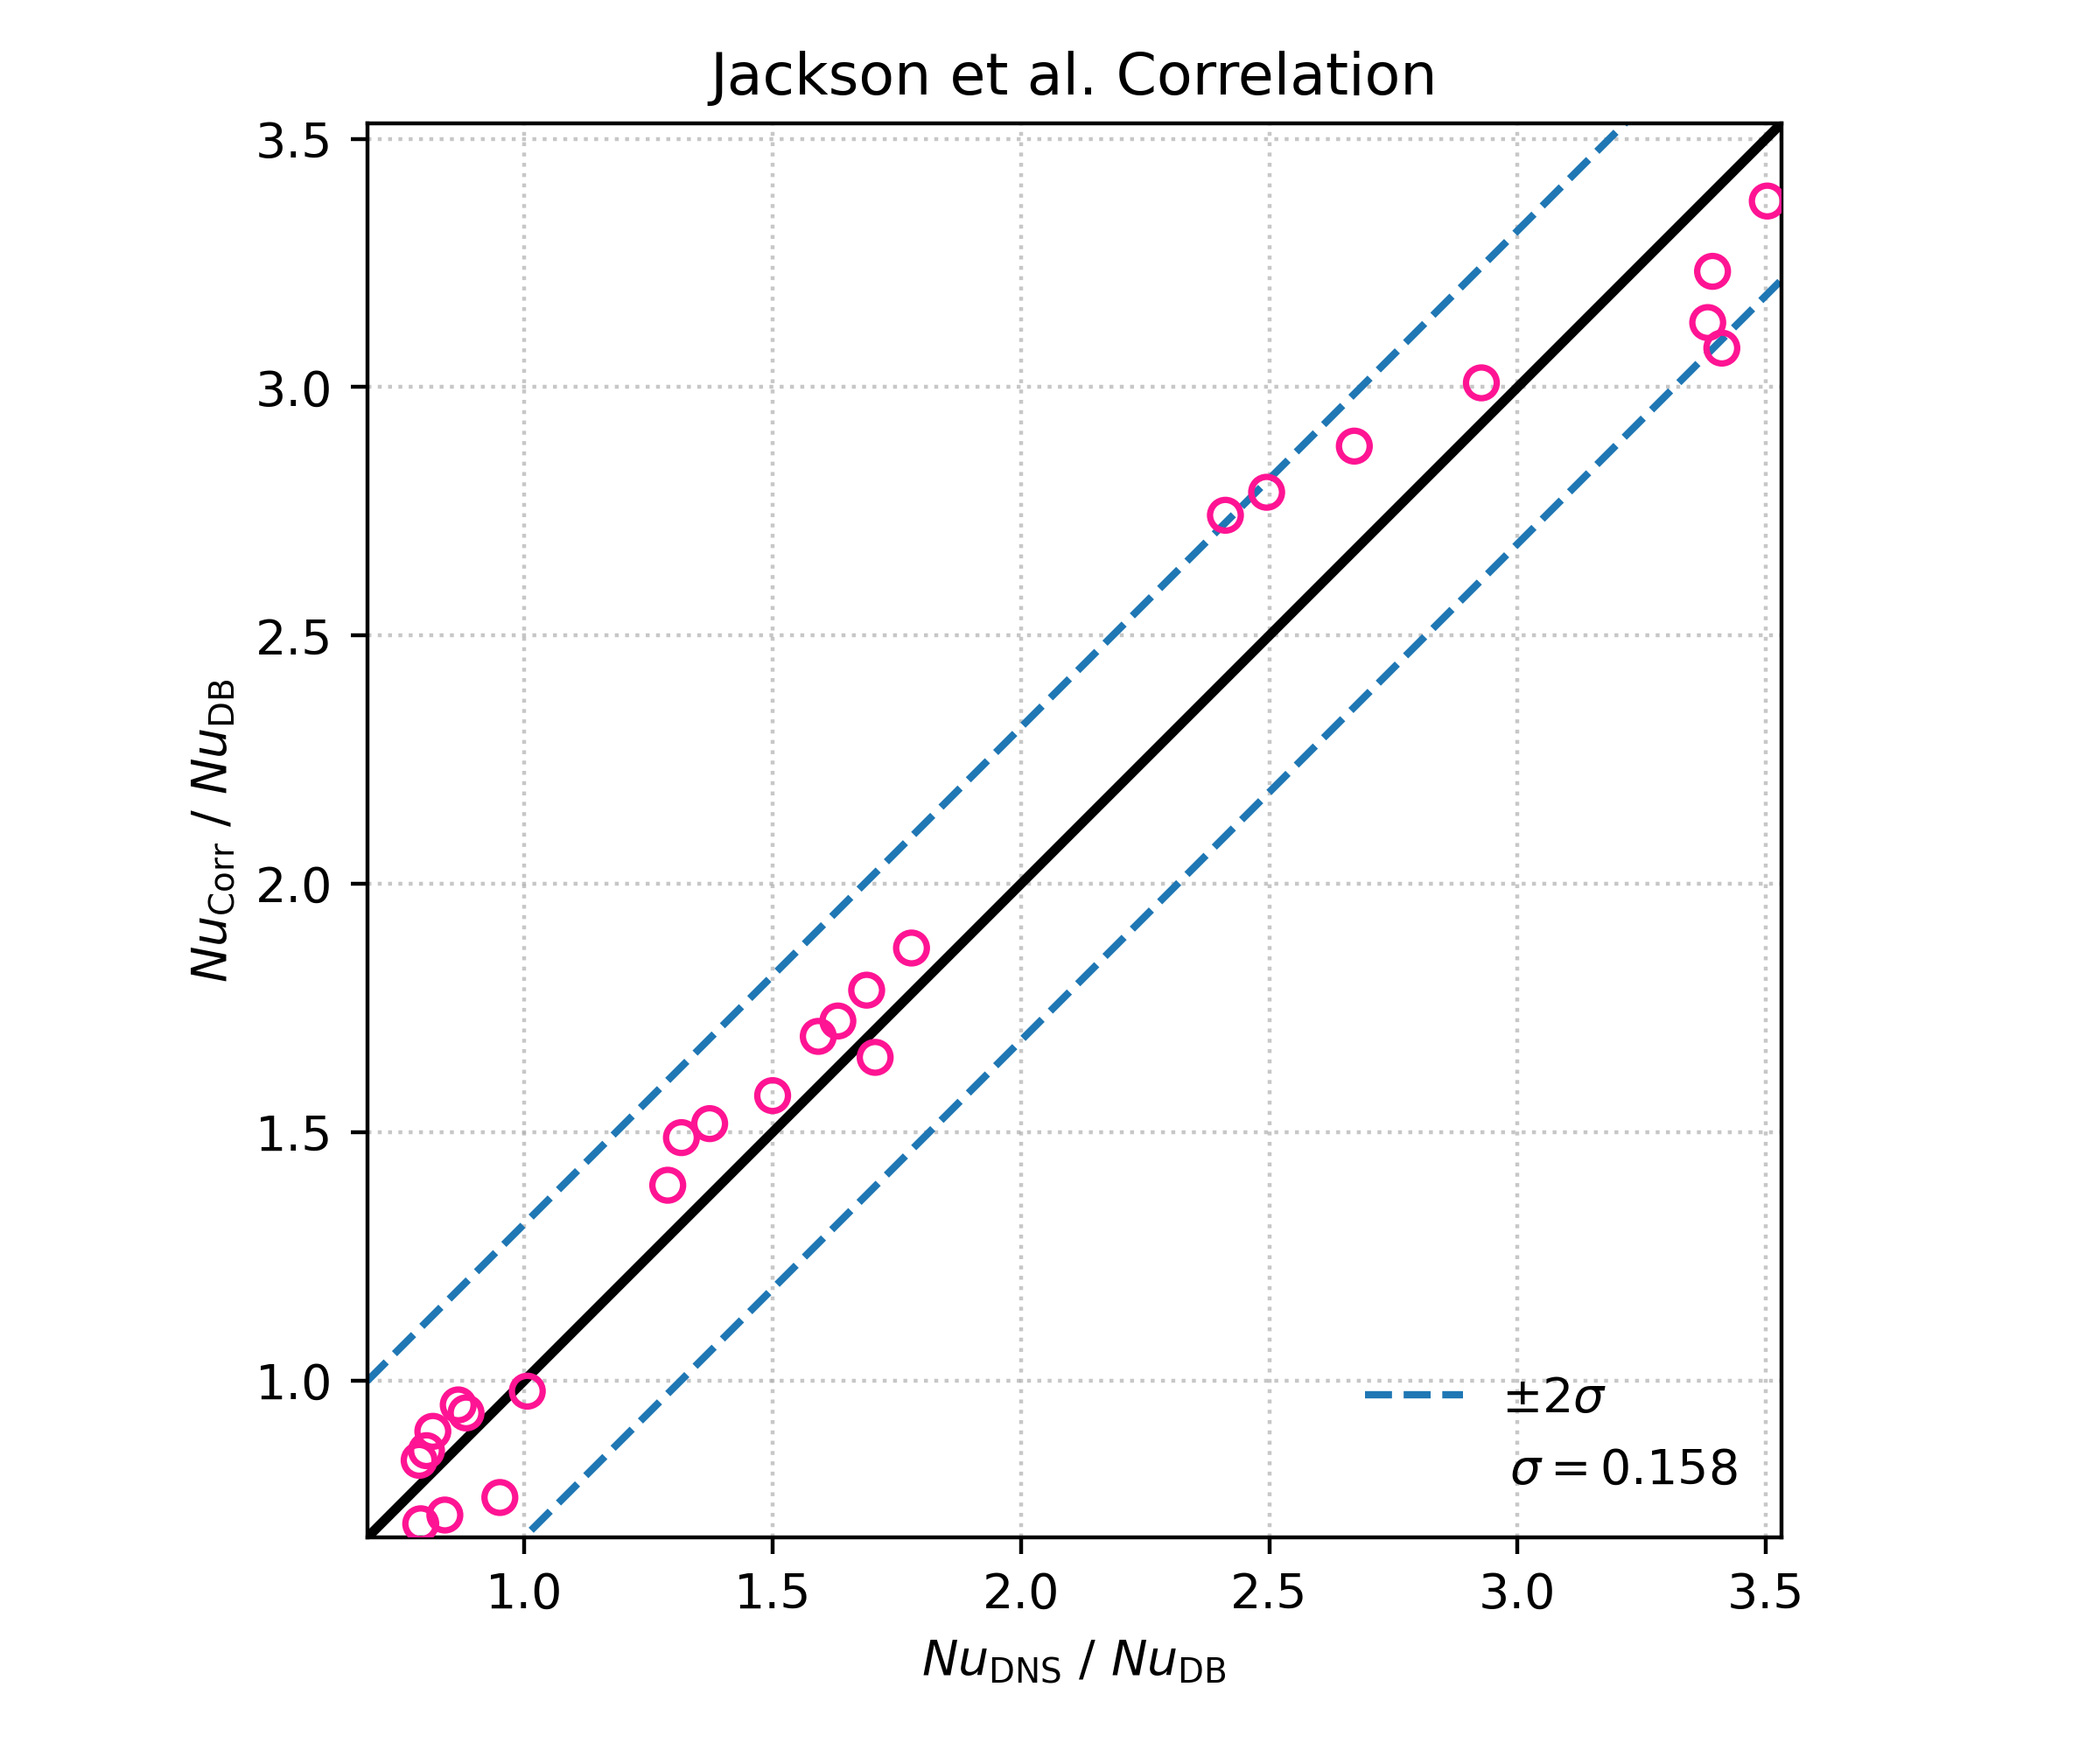
\includegraphics[width=0.49\textwidth]{figures/cap5/nusselt_corr/jackson_parity.png}
    \label{fig:parity}}
  \caption{\textbf{(a)} Número de Nusselt normalizado vs Bo; \textbf{(b)} paridad con la correlación de Jackson \textit{et al.}}
  \label{fig:nusselt}
\end{figure}



La disminución de Nu al aumentar la fuerza boyante puede entenderse a partir del perfil de velocidad en la dirección del flujo. Como se menciona en la sección \ref{sec:velo_temp}, cuando la convección natural y forzada actúan en la misma dirección, el fluido se acelera junto a las paredes y, por conservación de masa, se desacelera en la región central. En virtud de esta premisa, es posible acercarse a un entendimiento cualitativo. De acuerdo al modelo de Prandtl \cite{Prandtl1942}, la transferencia de calor se divide en dos mecanismos principales: (i) conducción en la subcapa viscosa y (ii) flujo de calor turbulento normal a la pared, $q''_y \approx \rho \, c_P \, \langle u^{*'}_y \theta^{*'} \rangle$. Algunos autores \cite{aicher1997, hall1969laminarization} sugieren que en el borde de la subcapa viscosa,  $q''_y$ es proporcional a la producción de turbulencia, cuya principal contribución recae en la producción por cizalla $\mathcal{P}$ (\textit{Shear-Production}). Sin embargo, también debe considerarse (aunque en menor medida) la contribución de la producción por boyancia $\mathcal{B}$ (\textit{Buoyancy-Production}). Los términos $\mathcal{P}$ y $\mathcal{B}$ provienen del balance de energía cinética turbulenta $k$  (véase el Apéndice \ref{apen:budgets}). El primero está ligado a diferencia de velocidades entre el centro del canal y la zona próxima a la pared, es decir, a un gradiente de velocidades.

Así, es posible apreciar un rango de Ri$_b$, correspondiente al intervalo $10^{-6}$ $\lesssim$ Bo $\lesssim$ $3 \times 10^{-5}$ en la Figura \ref{fig:nu_vs_bo}, para los cuales la aceleración inducida por la boyancia produce que esta diferencia de velocidades, o bien sea cero, o bien sea muy pequeña. Como consecuencia, disminuyen la producción turbulenta, el flujo de calor turbulento y, por lo tanto, Nu. Cuando la fuerza boyante continúa creciendo más allá de este intervalo, el gradiente de velocidad vuelve a incrementarse, la producción de turbulencia se intensifica y tanto $q''_y$ como Nu aumentan nuevamente. 

Esta última cuestión puede confirmarse al observar las Figuras \ref{fig:shear_prod} y \ref{fig:buoya_prod} donde se exponen los perfiles medios de $\mathcal{P}$ y $\mathcal{B}$, respectivamente, de los casos con Re$_o$=5000 y Pr=0.71. Se aprecia que valores moderados bajos de Ri$_b$ los perfiles tienen a decaer cerca de la pared, reduciendo la producción de turbulencia. Además, en general, se observa que la magnitud $\mathcal{B}$ es al menos un orden de magnitud menor y porque no tiene un rol tan relevante en la producción de turbulencia.

\begin{figure}[H]
  \centering
  \subfloat[]{
    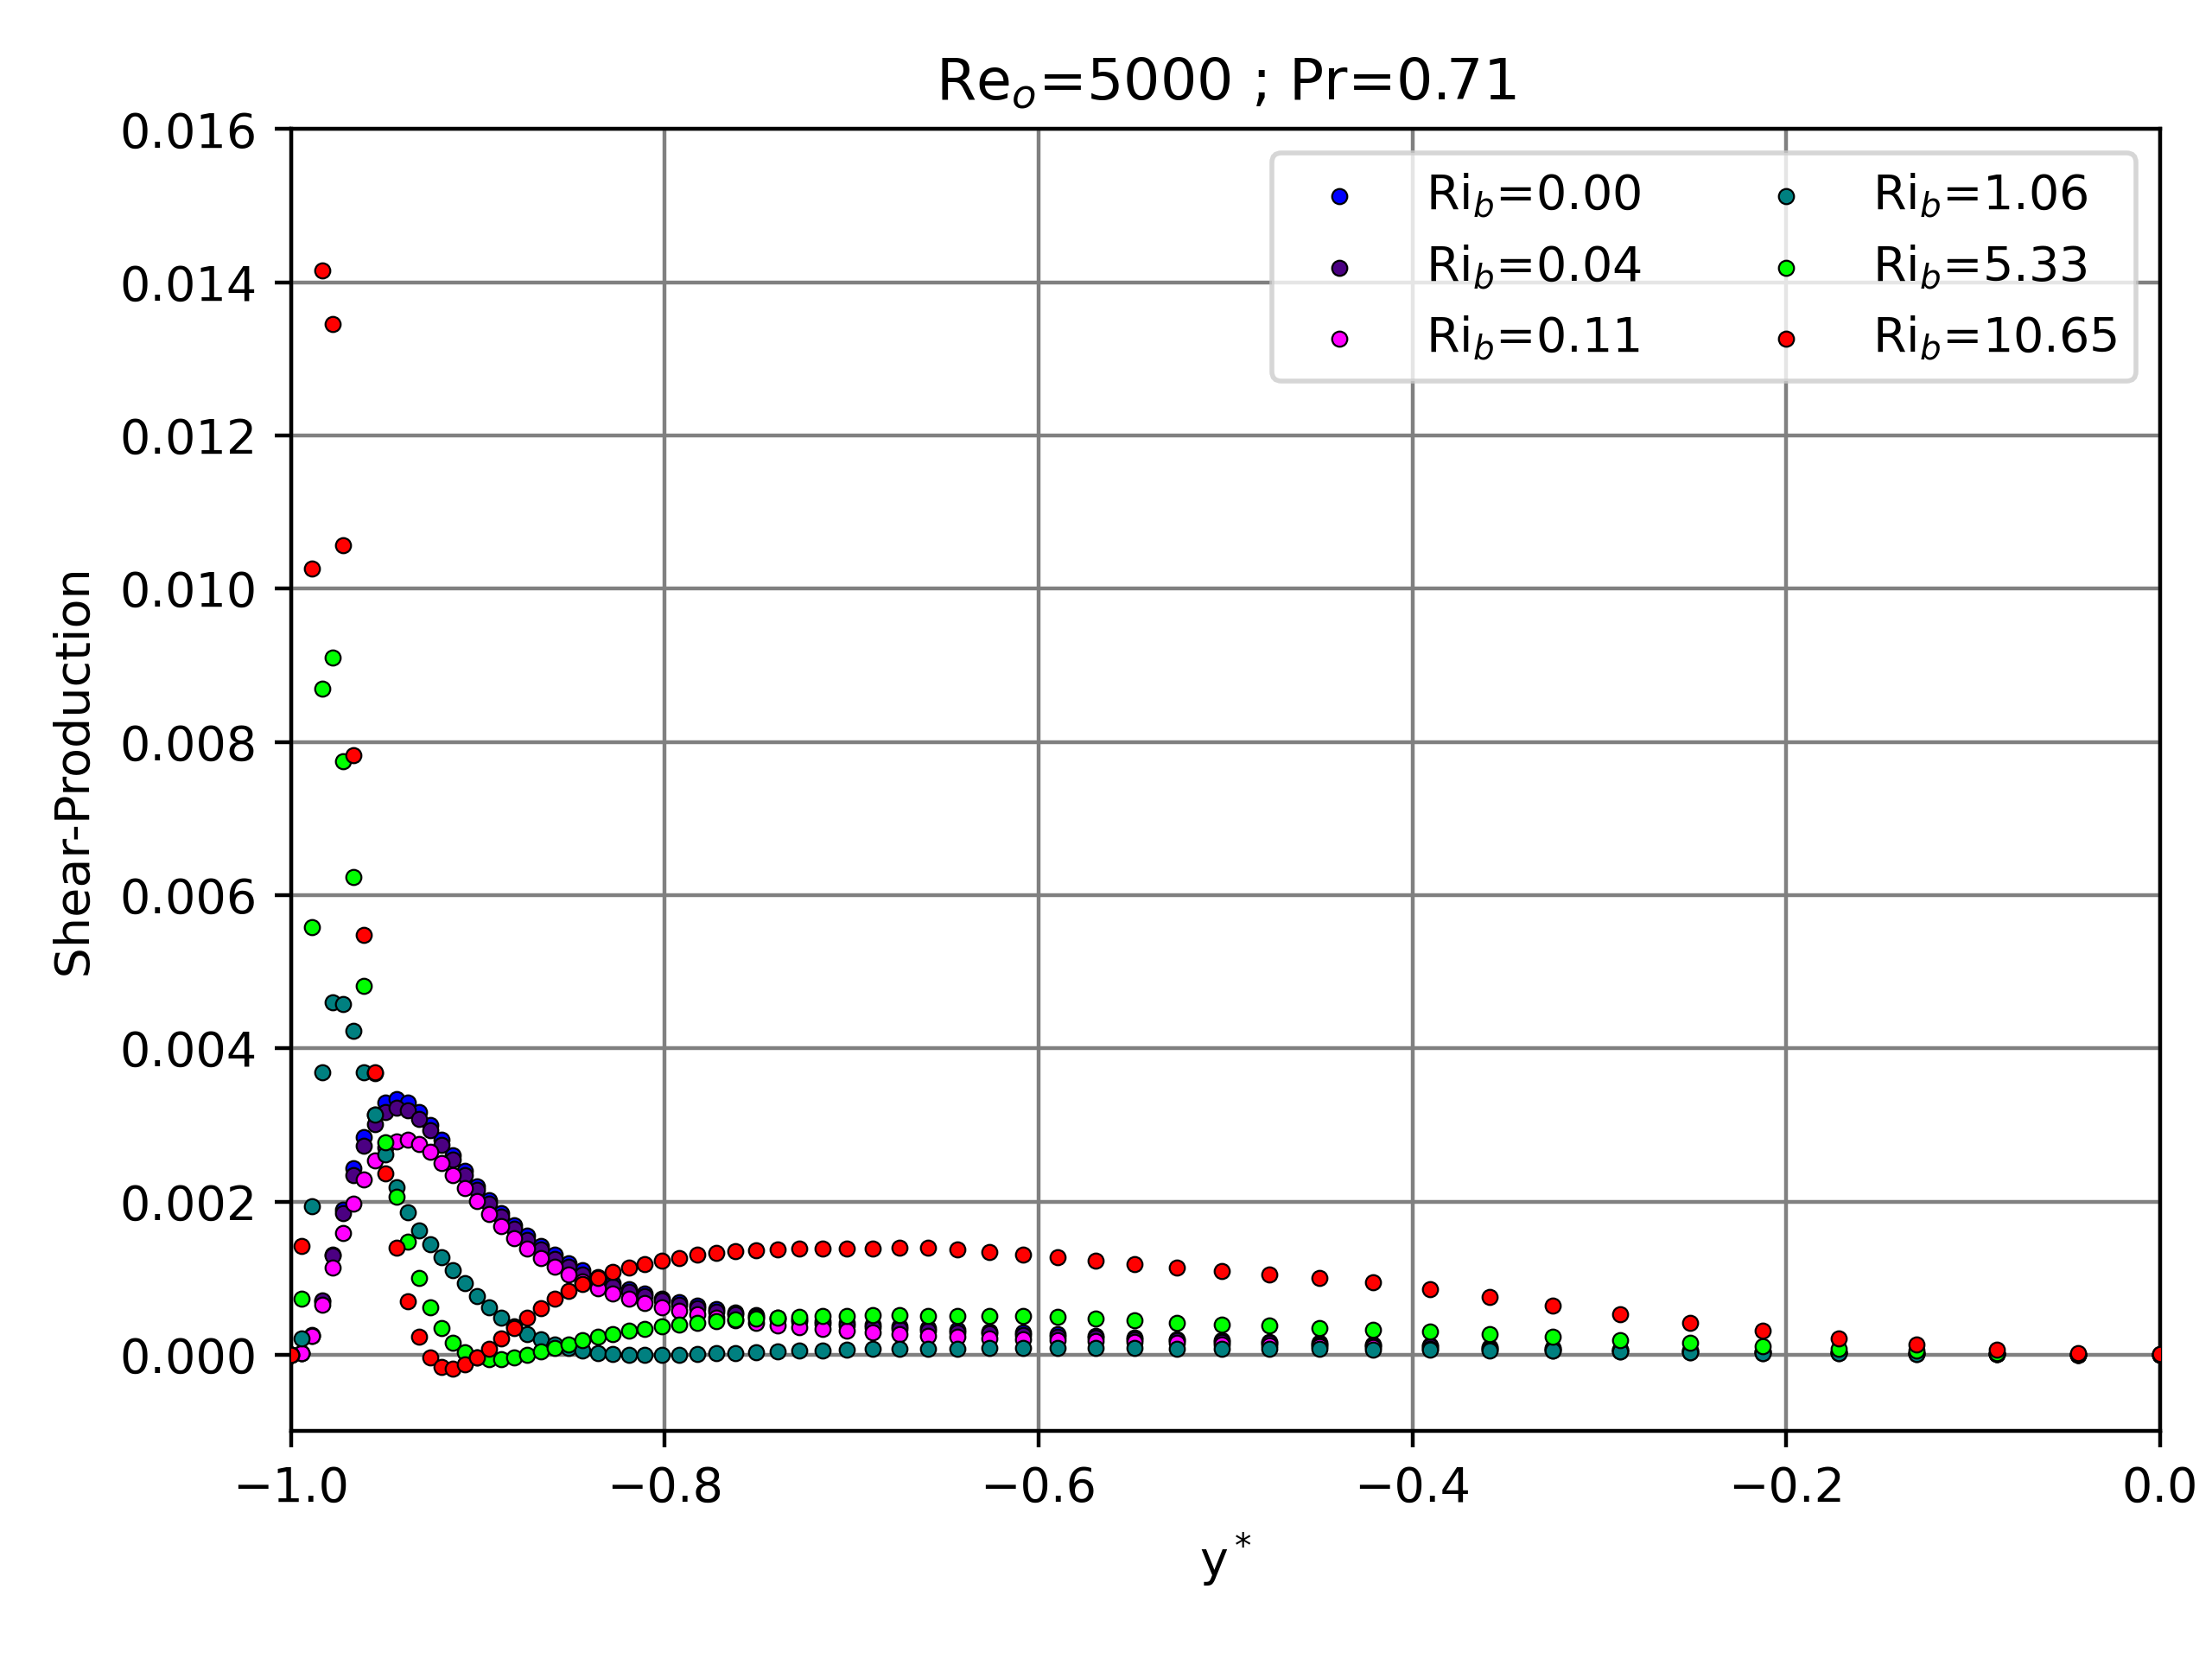
\includegraphics[width=0.49\textwidth]{figures/cap5/Re5000-Pr071-Ri1Em3_shear_prod.png}
    \label{fig:shear_prod}}
  \subfloat[]{
    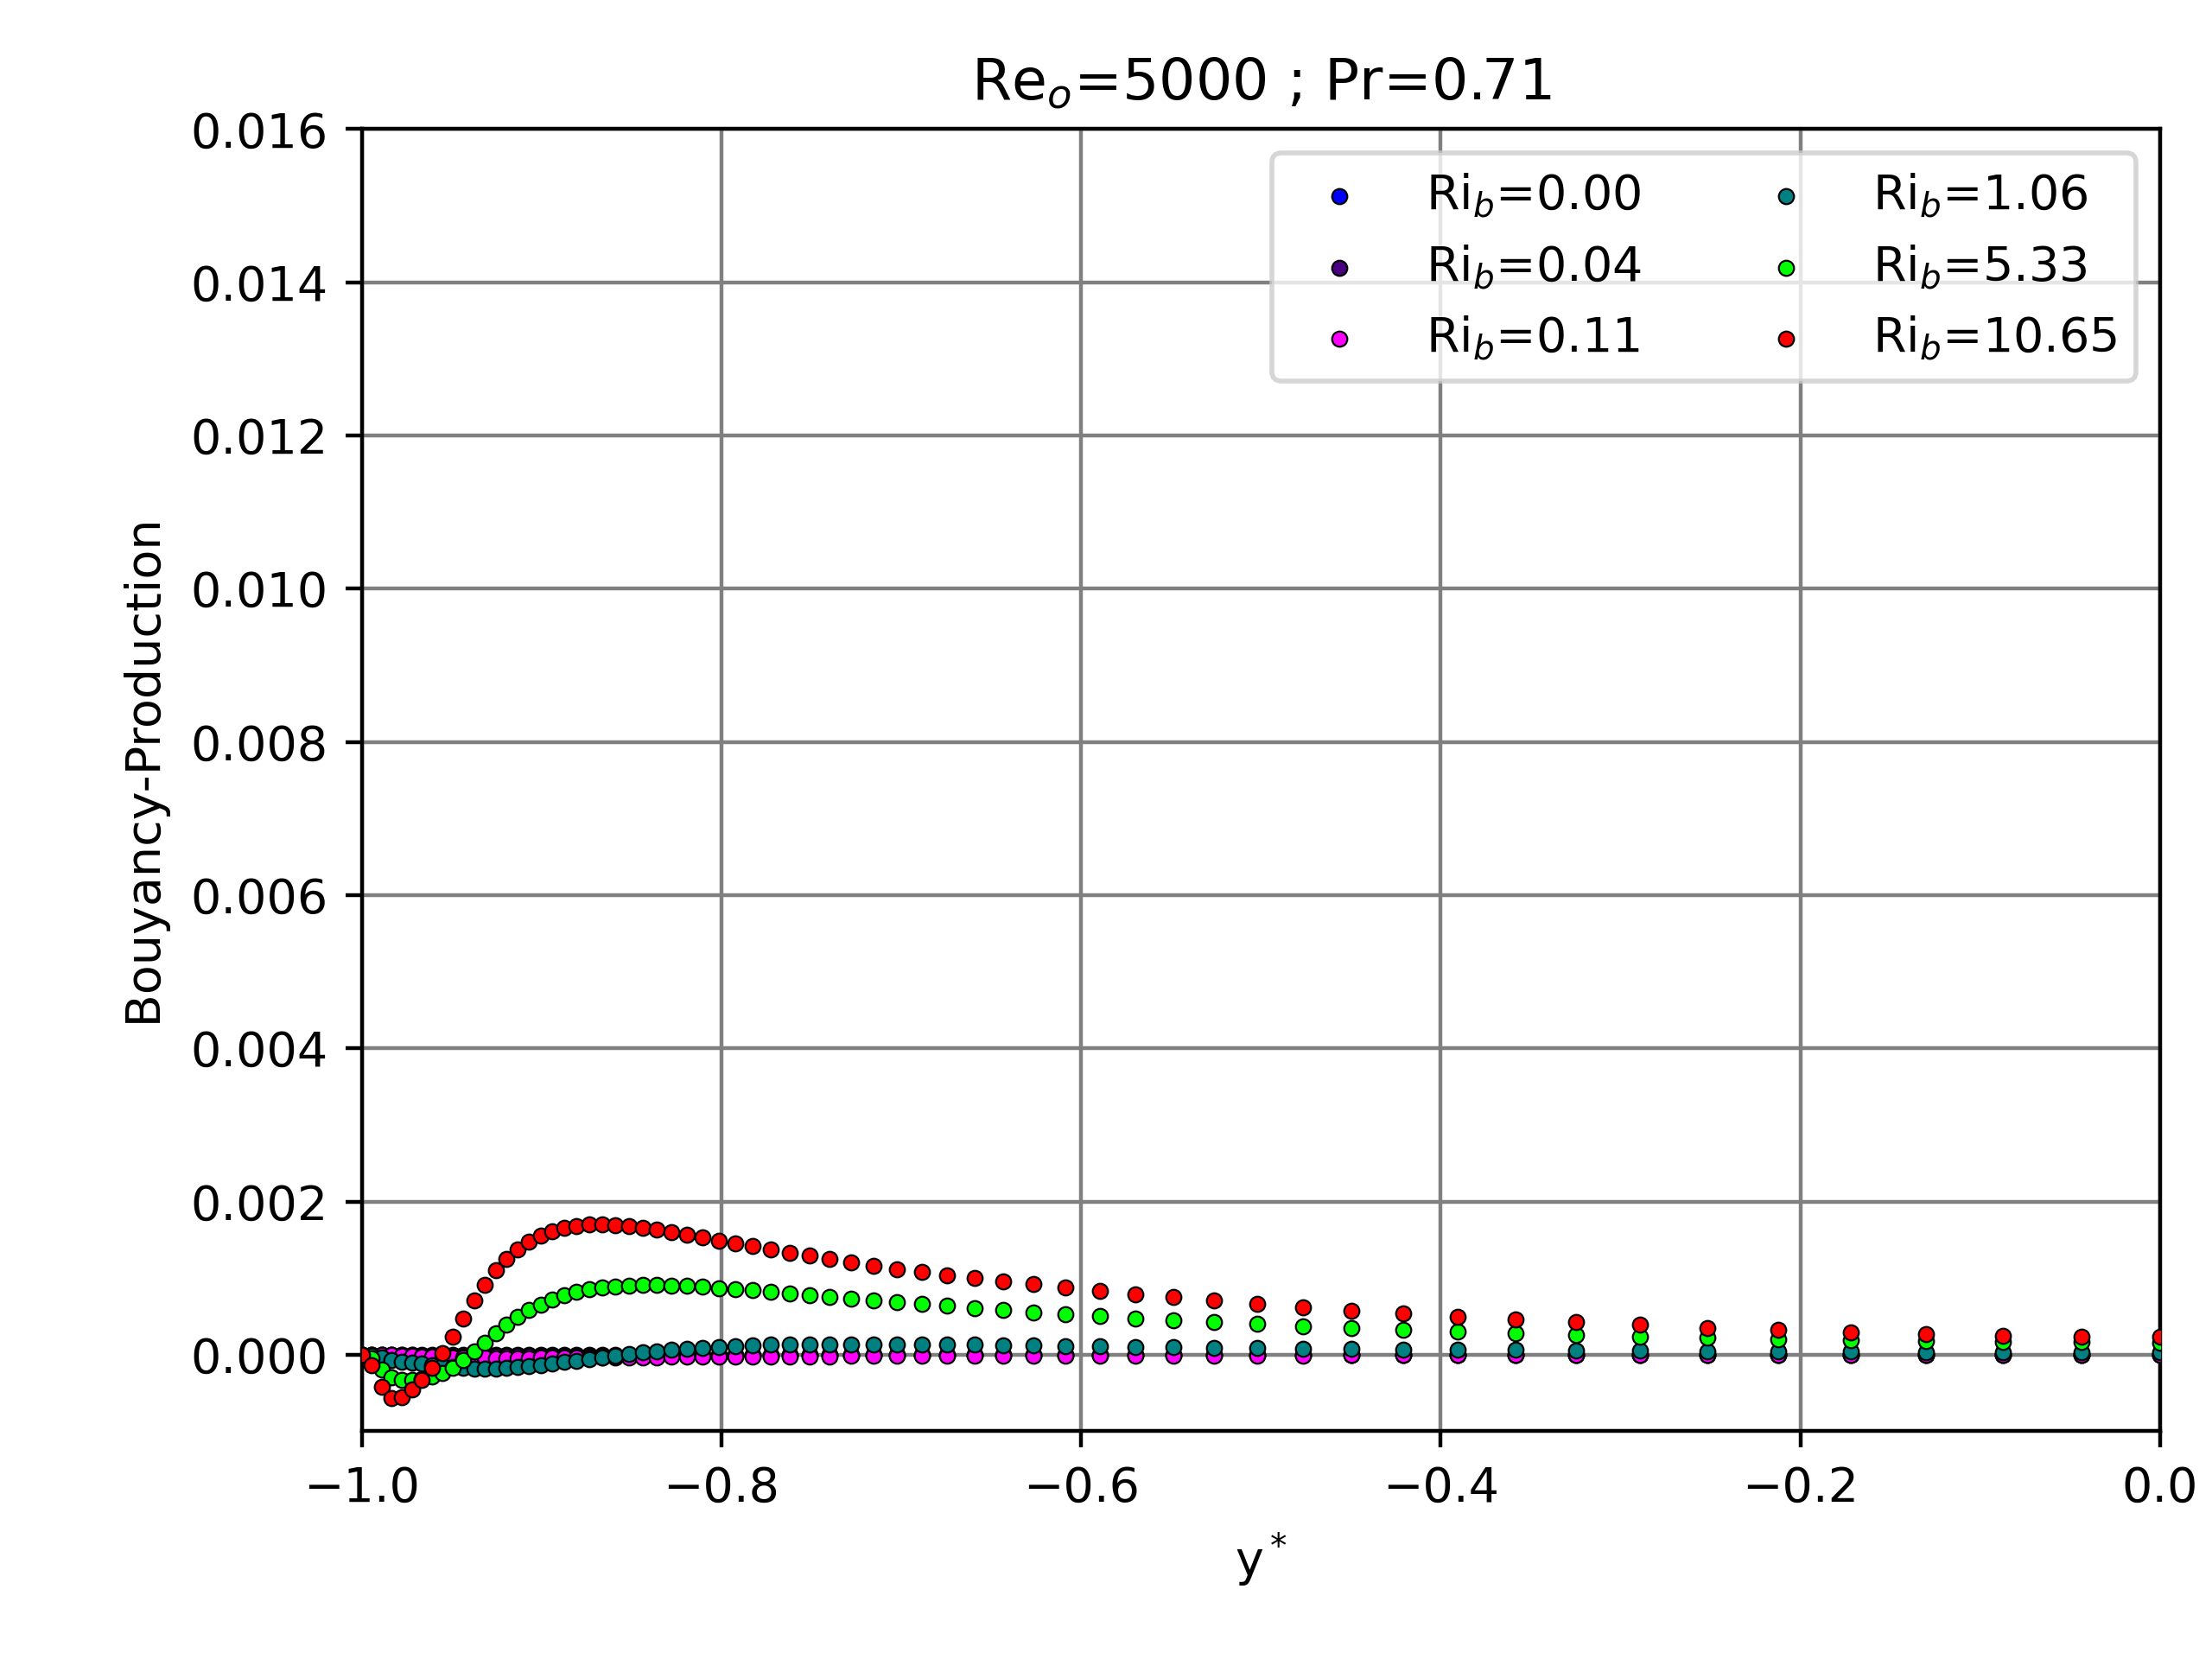
\includegraphics[width=0.49\textwidth]{figures/cap5/Re5000-Pr071-Ri1Em3_buoya_prod.png}
    \label{fig:buoya_prod}}
  \caption{Producción de energía cinética turbulenta: \textbf{(a)} componente por cizalla $\mathcal{P}$ y \textbf{(b)} contribución de la fuerza boyante $\mathcal{B}$.}
  \label{fig:budgets_prod}
\end{figure}


Como se analizará en la sección \ref{sec:nu}, en el primer conjunto la transferencia de calor por convección se deteriora, mientras que en el segundo conjunto dicha transferencia se recupera e incluso mejora respecto al caso de convección forzada pura. Estas observaciones, que no resultan intuitivas a primera vista, se esclarecen al examinar la Figura \ref{fig:uphi-Re5000-Pr071}, donde se representa el perfil medio $\langle u_x^{*}\theta^{*}\rangle$. El número de Nusselt es inversamente proporcional a $\langle\theta^{*}_b\rangle$ (ecuación \ref{eq:nu}), magnitud que depende del comportamiento de $\langle u_x^{*}\theta^{*}\rangle$. En consecuencia, un aumento de la temperatura incrementa $\langle u_x^{*}\theta^{*}\rangle$ y, por lo tanto, eleva $\langle\theta^{*}_b\rangle$, lo que conlleva una disminución de Nu.

\begin{figure}[H] % usa [H] solo si necesitas anclarla y tienes \usepackage{float}
  \centering
  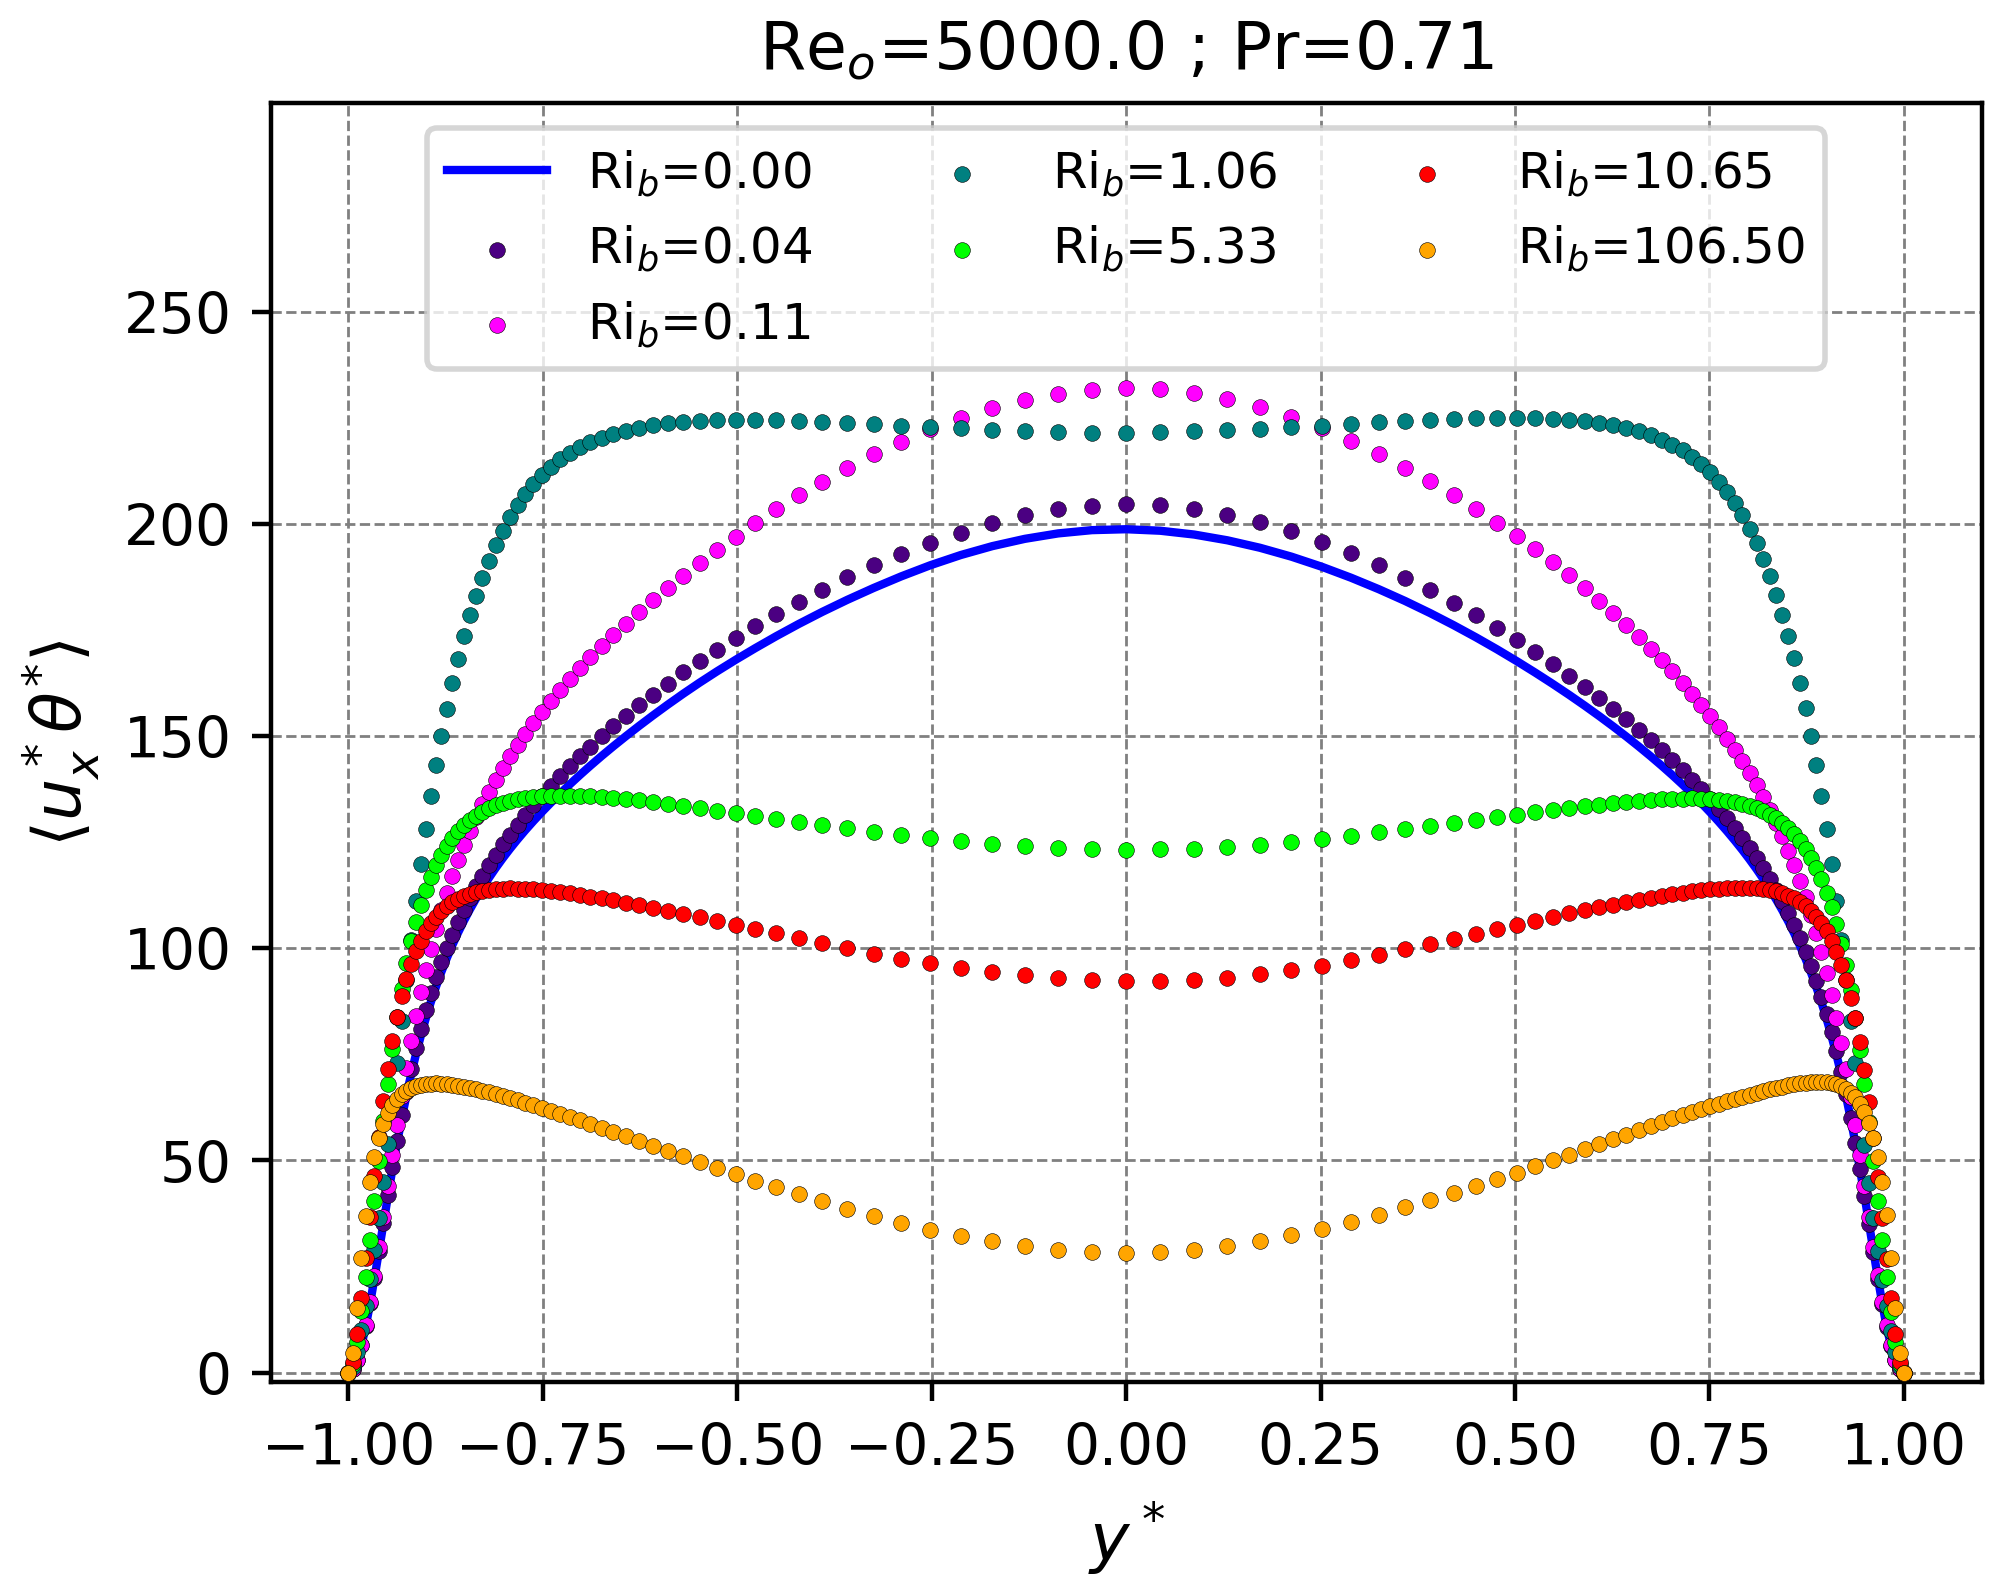
\includegraphics[width=0.6\textwidth]{figures/cap5/Re5000-Pr071/uxphi_profile.png}  
  \caption{Perfil de la magnitud media $\langle u^{*}_x\theta^{*}\rangle$.}
  \label{fig:uphi-Re5000-Pr071}
\end{figure}



Los cambios descritos en las fluctuaciones de temperatura y en el flujo turbulento $\langle u_x'\theta'\rangle$ repercuten directamente en la transferencia global de calor. En particular, la reducción de este flujo en el núcleo del canal para Bo$\lesssim3\times10^{-5}$ anticipa la caída del número de Nusselt, mientras que su posterior aumento (resultado de la mezcla intensificada por la fuerza boyante) explica la recuperación de $Nu$ a valores superiores al caso puramente forzado.




\newpage
\section{Factor de Fricción de Darcy}

En esta sección se analizan los resultados del coeficiente de fricción de Darcy. El mismo se define por la relación
\begin{equation}
f = 8 \frac{ \overline{\tau_w}}{\hspace{0.5mm} \rho \hspace{0.5mm} {U_b}^2 }  = \frac{18}{\text{Re}_o} \left.\frac{d \langle u^*_x \rangle}{dy}\right\vert_{wall} \text{.}
\label{eq:darcy}
\end{equation}
La Figura \ref{fig:darcy_vs_bo} recoge los valores de $f$ obtenidos en nuestras simulaciones DNS para una amplia gama de números de Boyancia (ecuación \ref{eq:jackson_bo}). Se incluyen, además, datos experimentales de Parlatan et al. \cite{parlatan1996buoyancy} y de DNS de You et al. \cite{you2003direct}. La coincidencia de tendencias entre los tres conjuntos de datos es excelente. Por otro lado, la literatura ofrece pocas correlaciones para $f$ (o para el factor de Fanning) en flujo turbulento completamente desarrollado bajo régimen de convección mixta. Partiendo del planteo de Easby \textit{et al.} \cite{easby1978effect}, se propone una nueva forma funcional, dada por la ecuación \ref{eq:fcorr}, cuyos parámetros se ajustan con nuestros resultados.
\begin{equation}
f_{corr} = C_1 + C_2 \hspace*{0.5mm} \text{Bo}^n
\label{eq:fcorr}
\end{equation}

\begin{small}
$$
C_1 = 0.03071701 \quad ; \quad C_2 = 10.03126205 \quad ; \quad n = 0.56152207
$$
\end{small}

La Figura \ref{fig:darcy_parity} muestra el gráfico de paridad $f_{\text{DNS}}$ frente a $f_{\text{corr}}$. La desviación estándar es $\sigma$=0.018 y el total de nuestros puntos se sitúa dentro de la banda de error, lo que confirma la fiabilidad de la correlación incluso al compararla con los datos de referencia externos.

\begin{figure}[H]
  \centering
  \subfloat[]{
    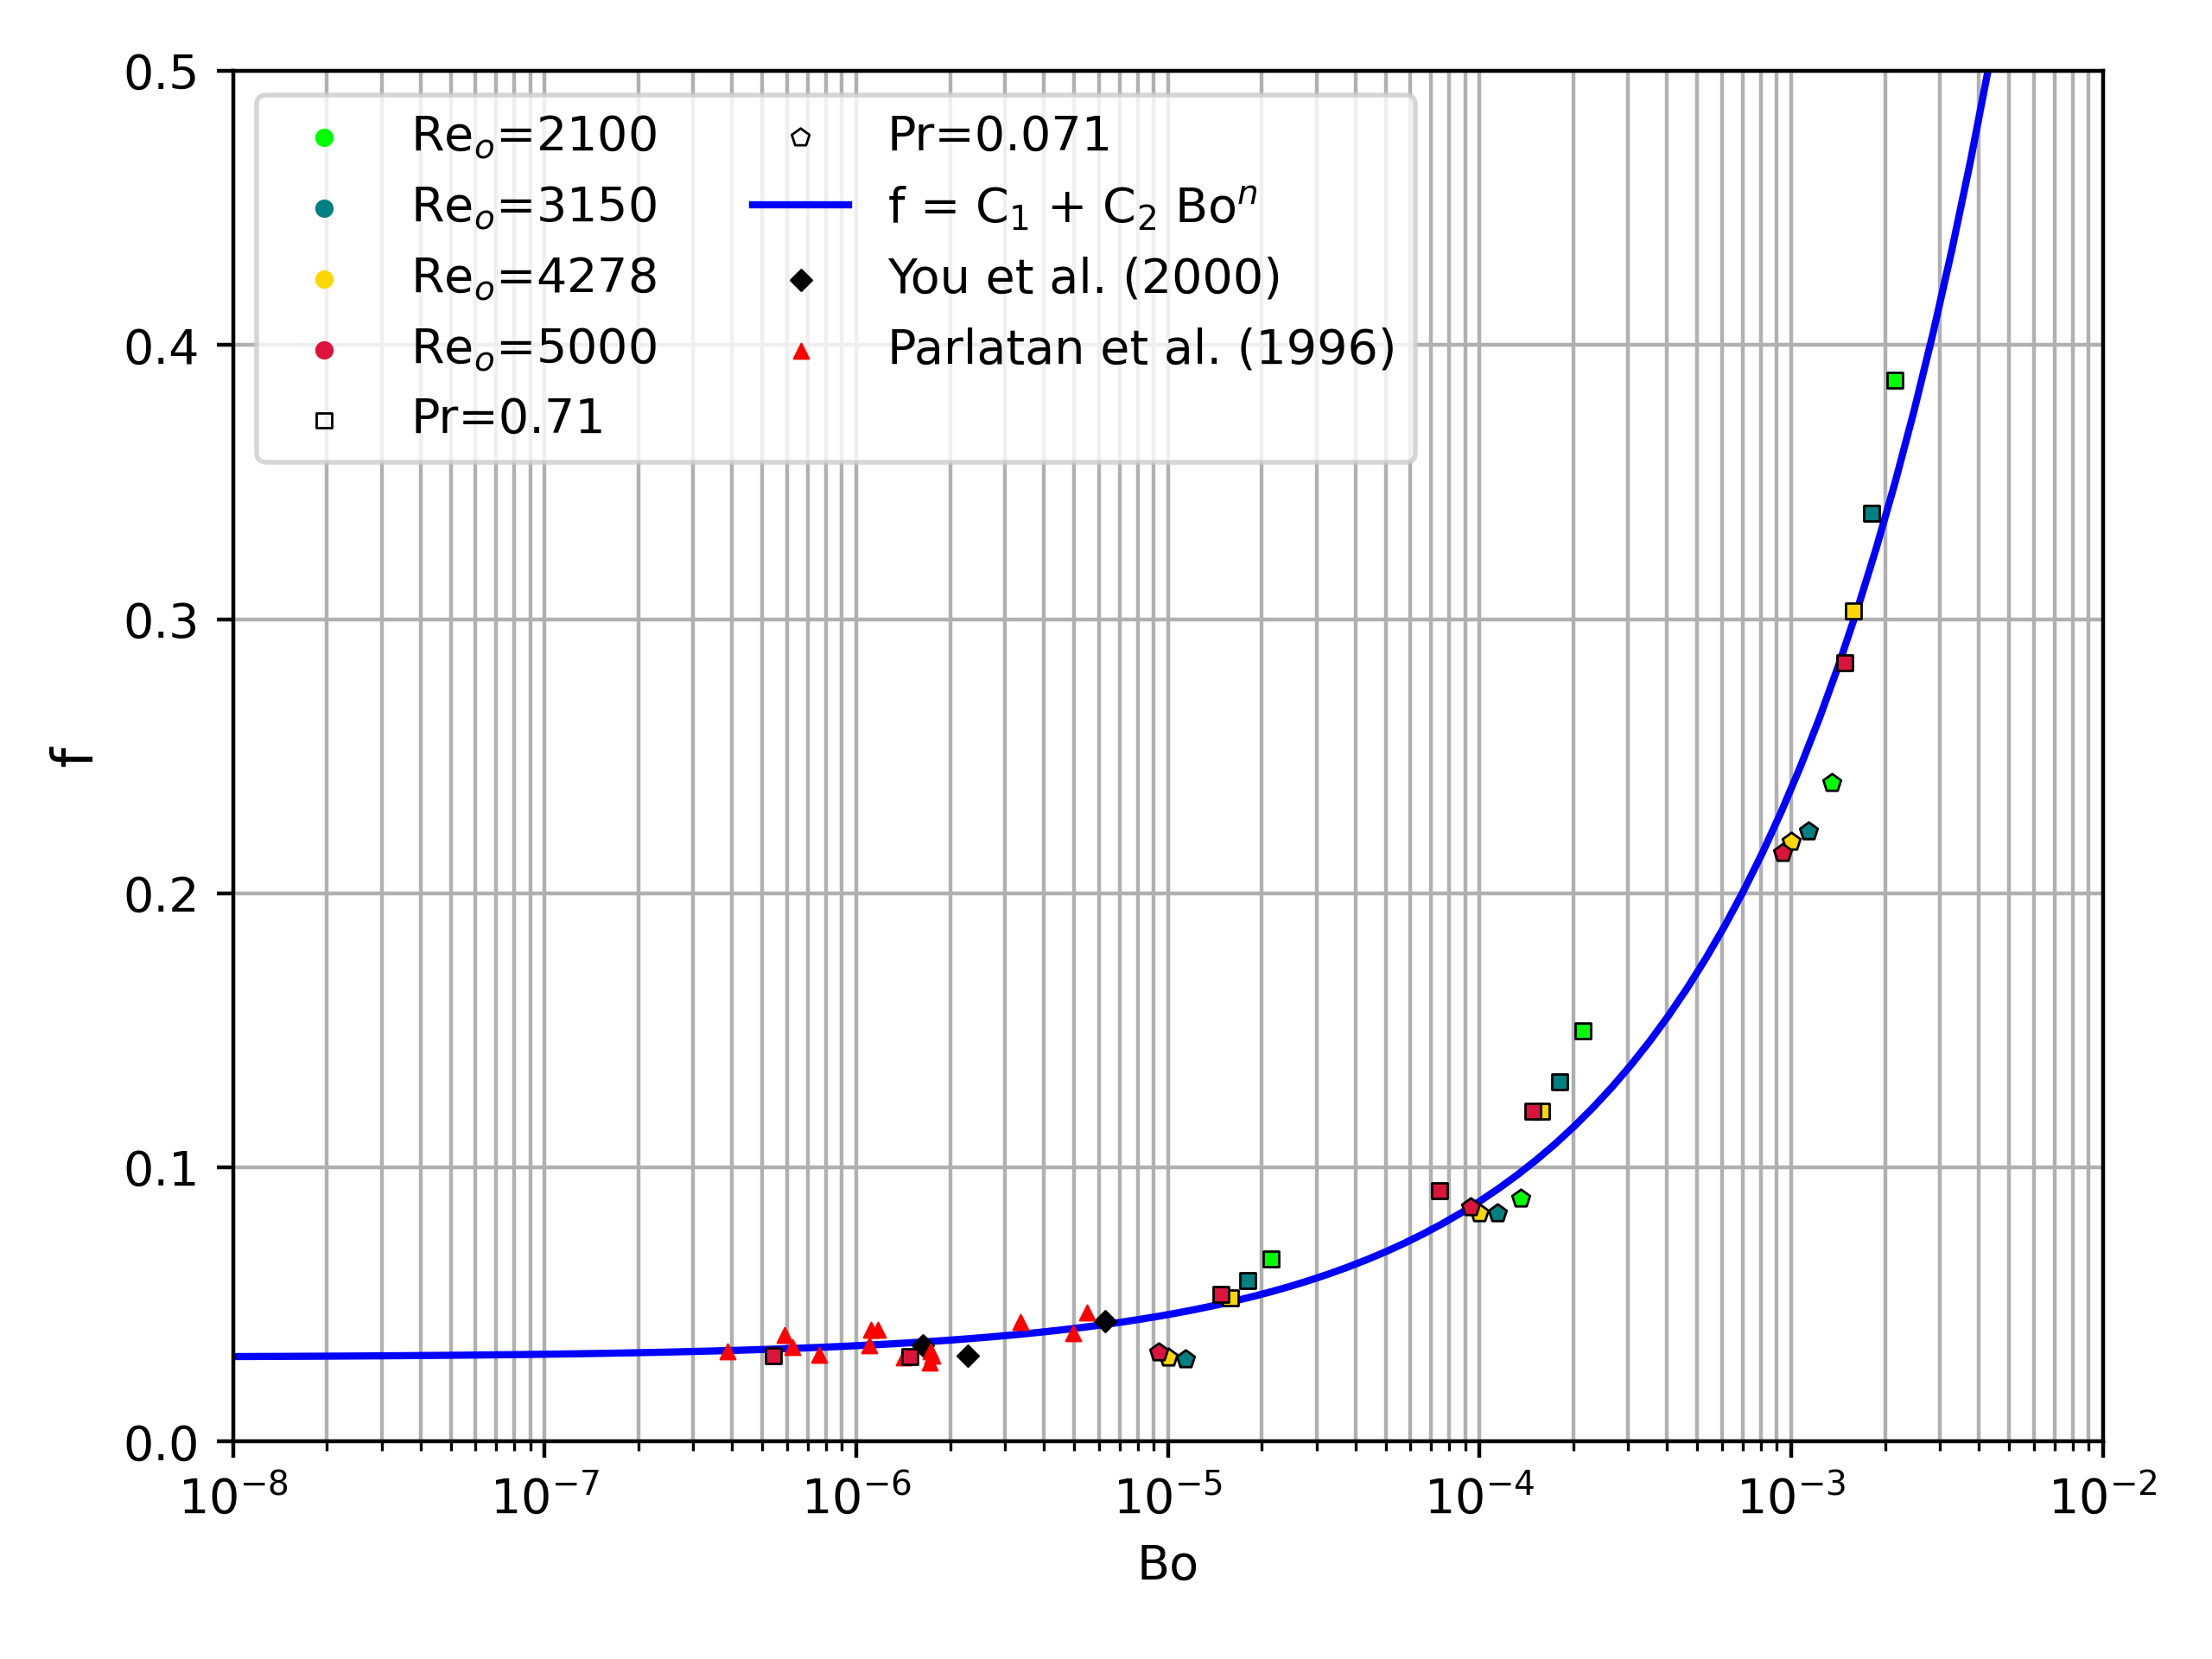
\includegraphics[width=0.49\textwidth]{figures/cap5/darcy/darcy_vs_Bo.png}
    \label{fig:darcy_vs_bo}}
  \subfloat[]{
    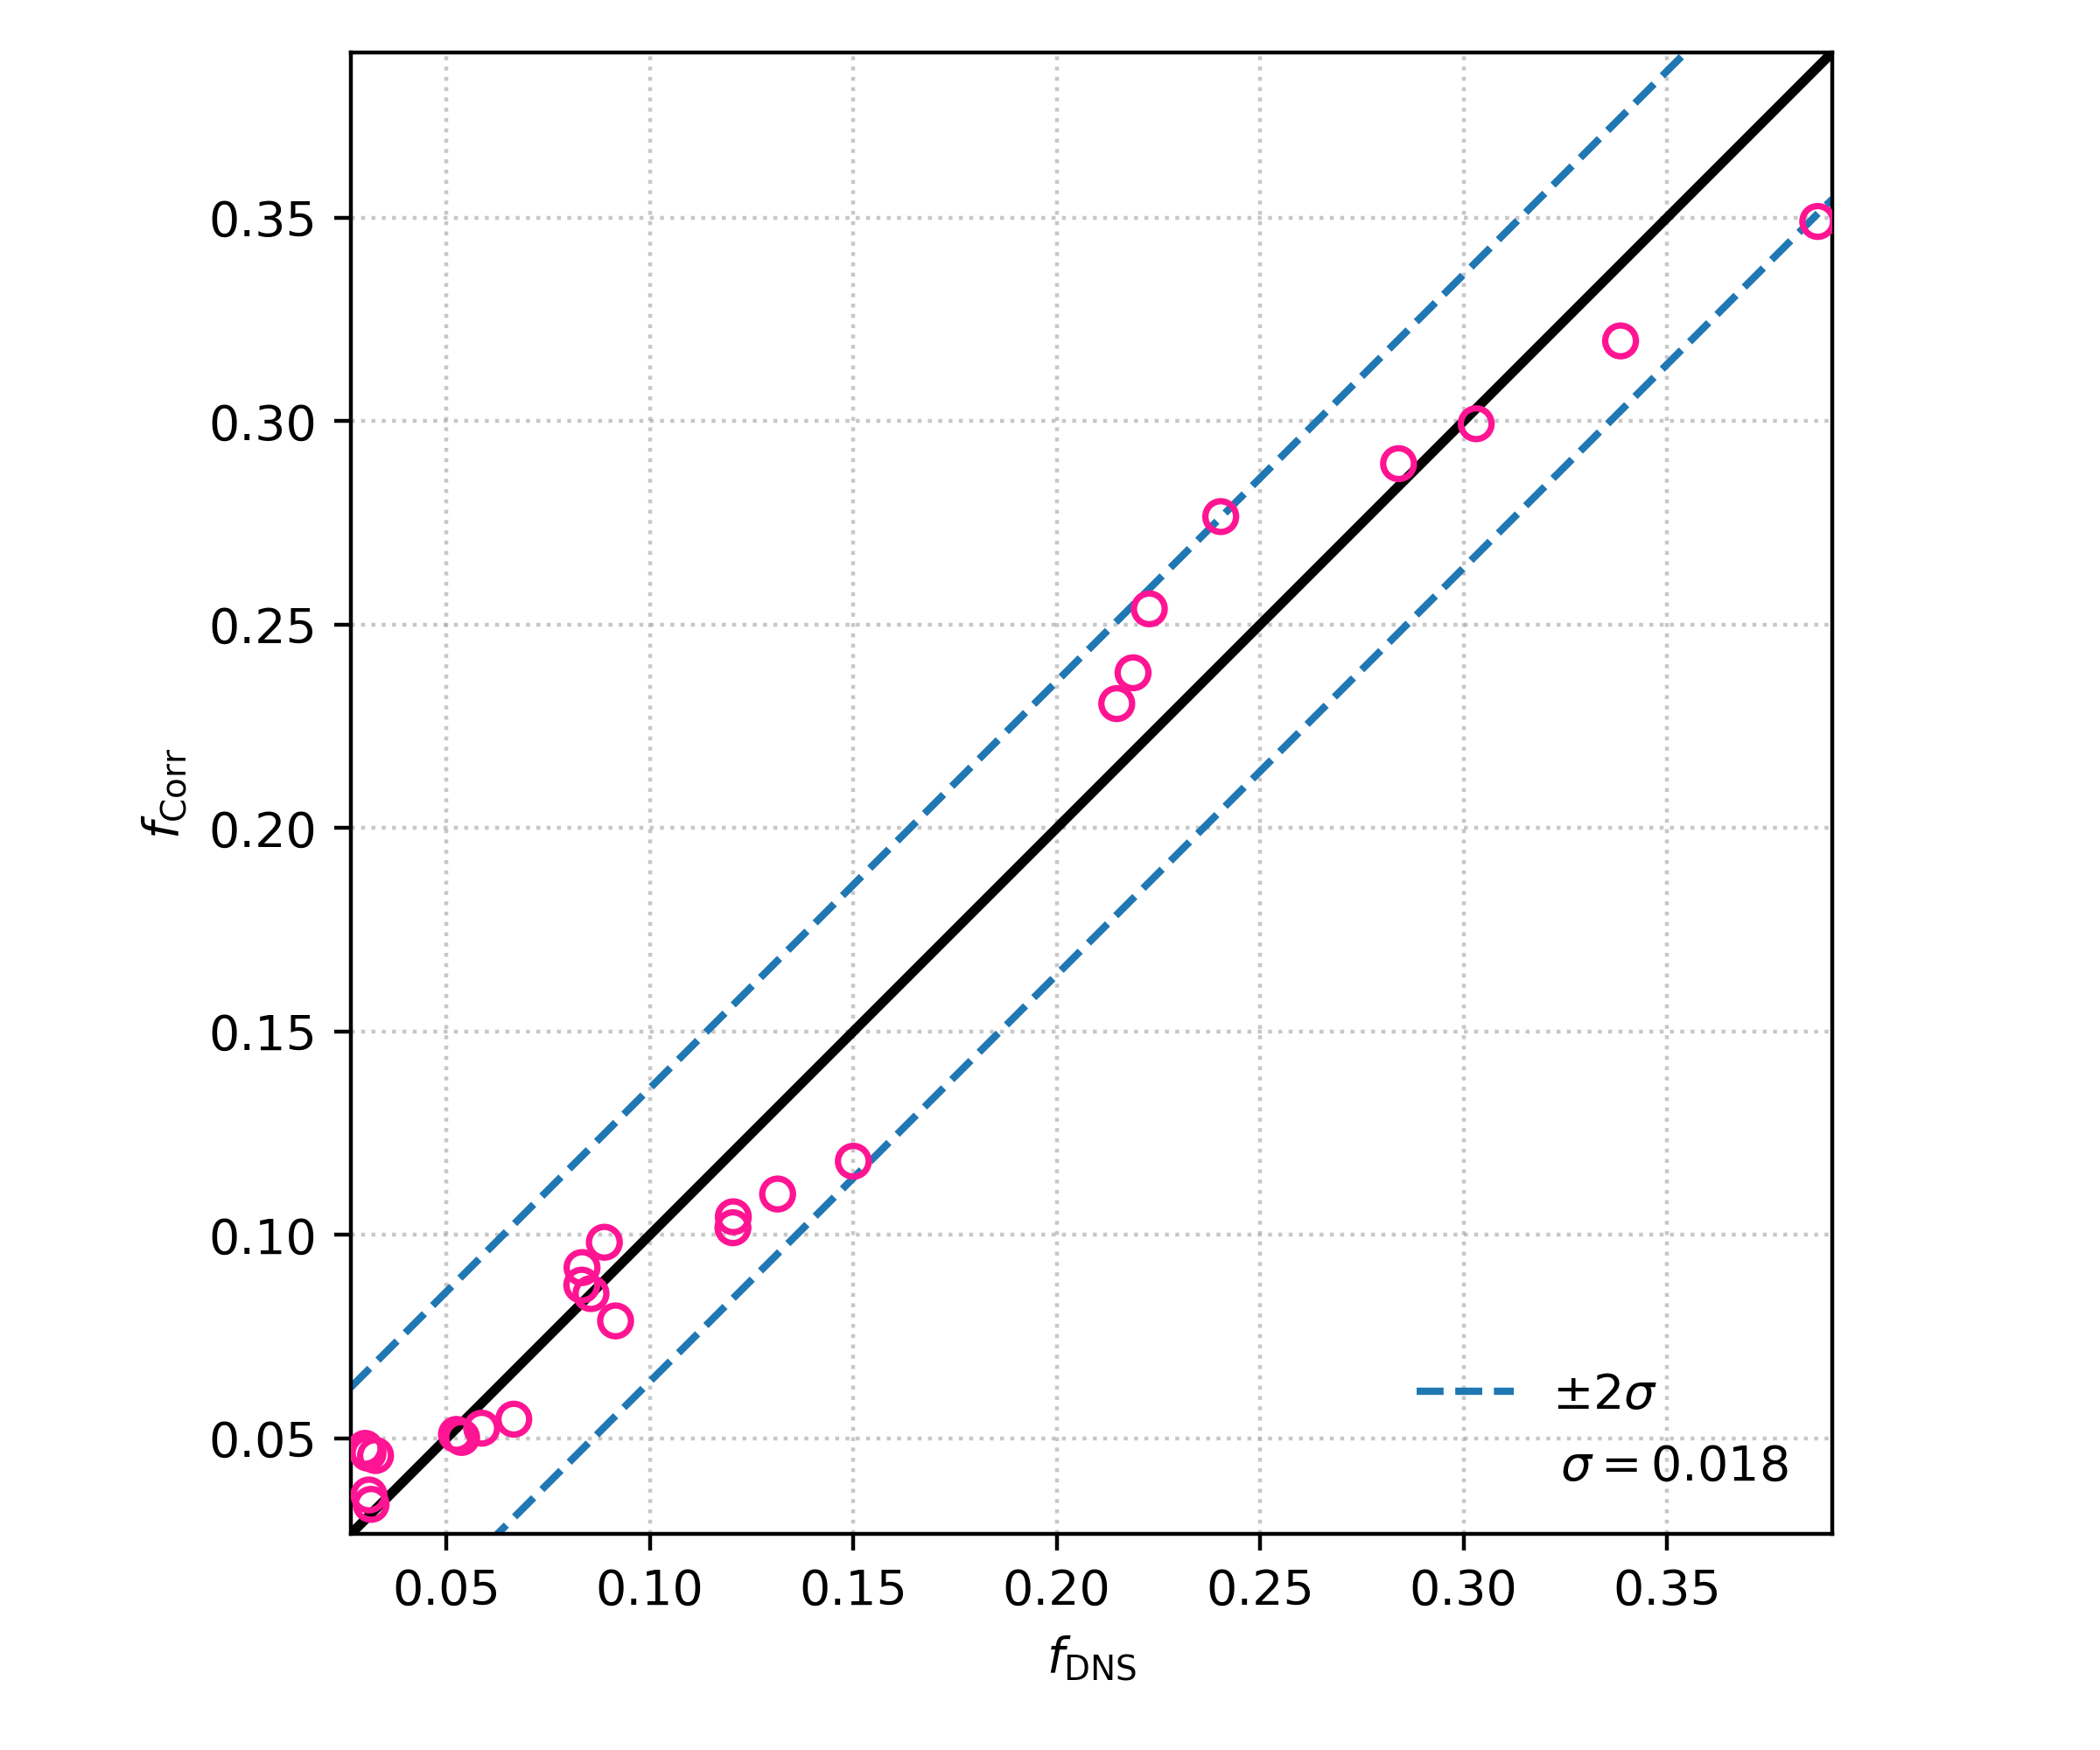
\includegraphics[width=0.49\textwidth]{figures/cap5/darcy/darcy_parity.png}
    \label{fig:darcy_parity}}
  \caption{Coeficiente de fricción de Darcy vs Bo y correlación propuesta; el ajuste reproduce los datos DNS/experimentales con $\sigma$ = 0.018.}
  \label{fig:nusselt}
\end{figure}

El incremento de $f$ con la boyancia parece, a priori, contraintuitivo: al actuar la fuerza boyante en la misma dirección del flujo cabría esperar menores pérdidas de carga. Sin embargo, los perfiles de velocidad mostrados en la sección \ref{sec:velo_temp} evidencian que la boyancia acelera el fluido en las zonas próximas a la pared, lo que incrementa la pendiente $d \langle u^*_x \rangle / dx^*$ y, por ende, la tensión cortante media $\overline{\tau_w}$. Este aumento local de cizalla compensa, e incluso supera, la ayuda proporcionada por la fuerza boyante, resultando en un valor mayor de $f$.


\section{Sumario de los principales hallazgos}

\begin{itemize}

\item \textbf{Perfiles de velocidad:} la fuerza boyante genera perfiles tipo ``M'' y desplaza el máximo de $\langle u_x\rangle$ hacia la pared.

\item \textbf{Perfiles de temperatura:} la mezcla inducida por la flotación ``aplana'' la temperatura media y reduce su fluctuaciones en el núcleo del canal.

\item \textbf{Degradación y mejora de Nu:} existe un intervalo $10^{-6}!\lesssim!Bo!\lesssim!3!\times!10^{-5}$ donde $Nu$ cae; fuera de él la transferencia se recupera y supera el caso puramente forzado.

\item \textbf{Mecanismo energético:} la caída de Nu coincide con una disminución en la producción de turbulencia cerca de la pared.

\item \textbf{Factor de Darcy creciente:} pese a la asistencia de la boyancia, el gradiente de velocidad en la pared aumenta y eleva el factor de Darcy; la correlación $f_{\text{corr}}=C_1+C_2 Bo^n$ reproduce los datos simulados propios, y los datos de referencia, con buena fidelidad.

\item \textbf{Efecto del Prandtl:} para Pr=0.071 la ley lineal de temperatura $\langle\theta^*\rangle \simeq \text{Pr} y^+$ se mantiene hasta $y^+ \approx 30$, mientras que para Pr=0.71 termina a $y^+ \approx 7$.
\end{itemize}